\documentclass[11pt, a4paper]{article}

% ============================================================================
% MODERN DOCUMENT SETUP - Sleek & Minimalistic Design
% ============================================================================

% Encoding and Language
\usepackage[utf8]{inputenc}
\usepackage[T1]{fontenc}

% Modern Typography - Clean Sans-Serif Look
\usepackage{lmodern}
\usepackage{helvet}  % Helvetica-style font
\renewcommand{\familydefault}{\sfdefault}  % Sans-serif as default

% Allow more flexible line breaking to reduce overfull boxes
\tolerance=1000
\emergencystretch=3em
\raggedbottom  % Allow flexible page bottoms to prevent vbox warnings

% Page Layout - Clean margins with breathing room
\usepackage[
    margin=1in,
    headheight=15pt,
    includehead,
    includefoot
]{geometry}

% Colors - Soft, Modern Palette
\usepackage{xcolor}

% Define modern color palette (muted, professional tones)
\definecolor{primaryBlue}{HTML}{4A90A4}      % Soft teal-blue
\definecolor{accentTeal}{HTML}{5DADE2}       % Light accent teal
\definecolor{softGreen}{HTML}{76D7C4}        % Muted green
\definecolor{warmOrange}{HTML}{F5B041}       % Soft orange accent
\definecolor{subtleGray}{HTML}{85929E}       % Muted gray
\definecolor{darkText}{HTML}{2C3E50}         % Dark blue-gray for text
\definecolor{lightBg}{HTML}{F8F9FA}          % Very light background
\definecolor{codeBg}{HTML}{FAFBFC}           % Code background
\definecolor{borderColor}{HTML}{E1E8ED}      % Soft border color

% GitHub-Like Diff Colors
\definecolor{ghDeletionBg}{HTML}{FFEBE9}     % Light red background
\definecolor{ghDeletionBorder}{HTML}{FF8182} % Red border
\definecolor{ghDeletionText}{HTML}{CF222E}   % Dark red text
\definecolor{ghAdditionBg}{HTML}{E6FFEC}     % Light green background
\definecolor{ghAdditionBorder}{HTML}{3FB950} % Green border
\definecolor{ghAdditionText}{HTML}{1A7F37}   % Dark green text
\definecolor{ghModifiedBg}{HTML}{FFF8E6}     % Light yellow background
\definecolor{ghModifiedBorder}{HTML}{D4A72C} % Yellow border
\definecolor{ghModifiedText}{HTML}{9A6700}   % Dark yellow text

% Graphics and Utilities
\usepackage{graphicx}
\usepackage{setspace}
\usepackage{parskip}
\usepackage{enumitem}

% Verbatim with line breaking
\usepackage{fancyvrb}
\usepackage{fvextra}

% Define custom verbatim environment with line breaking
\DefineVerbatimEnvironment{diffverb}{Verbatim}{
    fontsize=\footnotesize,
    breaklines=true,
    breakanywhere=true,
    breaksymbol={},
    breakautoindent=false
}

% Section Styling
\usepackage{titlesec}

% Modern Section Formatting
\titleformat{\section}
    {\LARGE\bfseries\color{primaryBlue}}
    {\thesection}{1em}{}
    [\vspace{-0.5em}\textcolor{accentTeal}{\rule{\linewidth}{1.5pt}}]

\titleformat{\subsection}
    {\Large\bfseries\color{darkText}}
    {\thesubsection}{1em}{}

\titleformat{\subsubsection}
    {\large\bfseries\color{subtleGray}}
    {\thesubsubsection}{1em}{}

% TikZ - Modern Flowcharts
\usepackage{tikz}
\usetikzlibrary{
    shapes.geometric,
    arrows.meta,
    shadows.blur,
    decorations.pathmorphing,
    positioning,
    calc,
    fit,
    bending,
    backgrounds
}

% Modern Node Styles - Soft gradients, subtle shadows, rounded aesthetics
\tikzset{
    % Base style for all nodes
    modern base/.style={
        font=\sffamily\small,
        align=center,
        text=darkText,
        minimum width=3.2cm,
        minimum height=1.1cm,
    },
    % Start/Stop nodes - Soft ellipse with gradient
    startstop/.style={
        modern base,
        ellipse,
        draw=primaryBlue,
        line width=1.5pt,
        top color=accentTeal!25,
        bottom color=accentTeal!8,
        blur shadow={
            shadow xshift=0.5ex,
            shadow yshift=-0.5ex,
            shadow blur steps=5,
            shadow opacity=25
        },
    },
    % Process nodes - Rounded rectangle with soft blue
    process/.style={
        modern base,
        rectangle,
        rounded corners=12pt,
        draw=primaryBlue!70,
        line width=1.2pt,
        top color=primaryBlue!18,
        bottom color=primaryBlue!5,
        blur shadow={
            shadow xshift=0.4ex,
            shadow yshift=-0.4ex,
            shadow blur steps=5,
            shadow opacity=20
        },
    },
    % Decision diamond - Soft green gradient
    decision/.style={
        modern base,
        diamond,
        aspect=2.2,
        draw=softGreen!80!darkText,
        line width=1.2pt,
        top color=softGreen!25,
        bottom color=softGreen!8,
        blur shadow={
            shadow xshift=0.4ex,
            shadow yshift=-0.4ex,
            shadow blur steps=5,
            shadow opacity=20
        },
        inner sep=2pt,
    },
    % IO nodes - Parallelogram style with warm accent
    io/.style={
        modern base,
        trapezium,
        trapezium left angle=70,
        trapezium right angle=110,
        draw=warmOrange!80!darkText,
        line width=1.2pt,
        top color=warmOrange!20,
        bottom color=warmOrange!5,
        blur shadow={
            shadow xshift=0.4ex,
            shadow yshift=-0.4ex,
            shadow blur steps=5,
            shadow opacity=20
        },
    },
    % Modern arrow style - Curved, soft color
    arrow/.style={
        -{Stealth[length=3mm, width=2mm, round]},
        line width=1mm,
        draw=primaryBlue!60,
        shorten >=3pt,
        shorten <=3pt,
        rounded corners=3pt,
    },
    % Dashed arrow variant
    arrow dashed/.style={
        arrow,
        dashed,
        draw=subtleGray!70,
        line width=0.8mm,
    },
    % Label style for YES/NO
    edge label/.style={
        font=\sffamily\scriptsize\bfseries,
        fill=white,
        inner sep=2pt,
        rounded corners=2pt,
    },
}

% Code Listings - Modern, clean styling
\usepackage{listings}
\lstset{
    language=Python,
    basicstyle=\ttfamily\footnotesize\color{darkText},
    keywordstyle=\color{primaryBlue}\bfseries,
    commentstyle=\color{softGreen!80!black}\itshape,
    stringstyle=\color{warmOrange!90!black},
    identifierstyle=\color{darkText},
    numbers=left,
    numberstyle=\tiny\color{subtleGray},
    numbersep=12pt,
    frame=none,
    backgroundcolor=\color{codeBg},
    breaklines=true,
    breakatwhitespace=false,
    breakautoindent=false,
    postbreak=\mbox{\textcolor{subtleGray}{$\hookrightarrow$}\space},
    showstringspaces=false,
    tabsize=4,
    captionpos=b,
    xleftmargin=20pt,
    xrightmargin=10pt,
    framexleftmargin=15pt,
    aboveskip=15pt,
    belowskip=10pt,
    emph={self,cls,__init__,__name__,True,False,None,def,class,import,from,return,if,else,elif,for,while,with,try,except,finally,async,await},
    emphstyle=\color{primaryBlue}\bfseries,
    emph=[2]{print,len,range,enumerate,zip,map,filter,sum,min,max,sorted,isinstance,hasattr,getattr,setattr,input,open,str,int,float,list,dict,set,tuple},
    emphstyle=[2]\color{softGreen!70!black}\bfseries,
    literate={->}{$\rightarrow$}{2}
             {<-}{$\leftarrow$}{2},
}

% Code box wrapper with modern styling
\usepackage{tcolorbox}
\tcbuselibrary{skins, breakable, listings}

% Modern code box style
\newtcolorbox{moderncode}{
    enhanced,
    breakable,
    colback=codeBg,
    colframe=borderColor,
    arc=8pt,
    boxrule=1pt,
    left=5pt,
    right=5pt,
    top=8pt,
    bottom=8pt,
    shadow={2pt}{-2pt}{0pt}{black!15},
}

% ============================================================================
% GITHUB-LIKE DIFF BOXES - Modern Aesthetic with Drop Shadows
% ============================================================================

% Diff boxes - Removed code (GitHub red theme)
\newtcolorbox{removedcode}[1][Removed Code]{
    enhanced,
    breakable,
    colback=ghDeletionBg,
    colframe=ghDeletionBorder,
    arc=8pt,
    boxrule=1.5pt,
    left=8pt,
    right=8pt,
    top=10pt,
    bottom=10pt,
    title={\textcolor{ghDeletionText}{\textbf{--- #1}}},
    fonttitle=\sffamily\bfseries\small,
    coltitle=ghDeletionText,
    attach boxed title to top left={yshift=-3mm, xshift=8mm},
    boxed title style={
        colback=ghDeletionBg,
        colframe=ghDeletionBorder,
        arc=4pt,
        boxrule=1pt,
    },
    drop shadow={
        shadow xshift=0.5ex,
        shadow yshift=-0.5ex,
        opacity=0.2,
        fill=ghDeletionBorder!50,
    },
    borderline west={4pt}{0pt}{ghDeletionBorder},
    before upper={\footnotesize},
}

% Diff boxes - Added code (GitHub green theme)
\newtcolorbox{addedcode}[1][Added Code]{
    enhanced,
    breakable,
    colback=ghAdditionBg,
    colframe=ghAdditionBorder,
    arc=8pt,
    boxrule=1.5pt,
    left=8pt,
    right=8pt,
    top=10pt,
    bottom=10pt,
    title={\textcolor{ghAdditionText}{\textbf{+++ #1}}},
    fonttitle=\sffamily\bfseries\small,
    coltitle=ghAdditionText,
    attach boxed title to top left={yshift=-3mm, xshift=8mm},
    boxed title style={
        colback=ghAdditionBg,
        colframe=ghAdditionBorder,
        arc=4pt,
        boxrule=1pt,
    },
    drop shadow={
        shadow xshift=0.5ex,
        shadow yshift=-0.5ex,
        opacity=0.2,
        fill=ghAdditionBorder!50,
    },
    borderline west={4pt}{0pt}{ghAdditionBorder},
    before upper={\footnotesize},
}

% Diff boxes - Modified code (GitHub orange/yellow theme)
\newtcolorbox{modifiedcode}[1][Modified Code]{
    enhanced,
    breakable,
    colback=ghModifiedBg,
    colframe=ghModifiedBorder,
    arc=8pt,
    boxrule=1.5pt,
    left=8pt,
    right=8pt,
    top=10pt,
    bottom=10pt,
    title={\textcolor{ghModifiedText}{\textbf{~~~ #1}}},
    fonttitle=\sffamily\bfseries\small,
    coltitle=ghModifiedText,
    attach boxed title to top left={yshift=-3mm, xshift=8mm},
    boxed title style={
        colback=ghModifiedBg,
        colframe=ghModifiedBorder,
        arc=4pt,
        boxrule=1pt,
    },
    drop shadow={
        shadow xshift=0.5ex,
        shadow yshift=-0.5ex,
        opacity=0.2,
        fill=ghModifiedBorder!50,
    },
    borderline west={4pt}{0pt}{ghModifiedBorder},
    before upper={\footnotesize},
}

% Inline diff highlighting commands
\newcommand{\diffrem}[1]{\colorbox{ghDeletionBg}{\textcolor{ghDeletionText}{\texttt{-}\,\texttt{#1}}}}
\newcommand{\diffadd}[1]{\colorbox{ghAdditionBg}{\textcolor{ghAdditionText}{\texttt{+}\,\texttt{#1}}}}
\newcommand{\diffmod}[1]{\colorbox{ghModifiedBg}{\textcolor{ghModifiedText}{\texttt{\textasciitilde}\,\texttt{#1}}}}

% Headers and Footers - Clean, minimal
\usepackage{fancyhdr}
\pagestyle{fancy}
\fancyhf{}
\fancyhead[R]{\textcolor{subtleGray}{\sffamily\small Code Documentation}}
\fancyfoot[C]{\textcolor{subtleGray}{\sffamily\small\thepage}}
\renewcommand{\headrulewidth}{0.5pt}
\renewcommand{\footrulewidth}{0pt}
\renewcommand{\headrule}{\hbox to\headwidth{\color{borderColor}\leaders\hrule height \headrulewidth\hfill}}

% Hyperlinks - Modern, subtle
\usepackage{hyperref}
\hypersetup{
    colorlinks=true,
    linkcolor=primaryBlue,
    urlcolor=accentTeal,
    citecolor=softGreen,
    pdfborder={0 0 0},
}

% Better list styling
\setlist[itemize]{
    topsep=8pt,
    itemsep=4pt,
    parsep=2pt,
    leftmargin=20pt,
}
\setlist[enumerate]{
    topsep=8pt,
    itemsep=4pt,
    parsep=2pt,
    leftmargin=20pt,
}

% Document Info
\title{%
    \vspace{-1cm}
    \textcolor{primaryBlue}{\rule{\linewidth}{2pt}}\\[0.8em]
    {\Huge\bfseries\sffamily\textcolor{darkText}{Comprehensive Code Documentation}}\\[0.3em]
    {\Large\sffamily\textcolor{subtleGray}{CSU2220 - Generative AI for Building Applications}}\\[0.5em]
    \textcolor{primaryBlue}{\rule{\linewidth}{2pt}}
}
\author{\sffamily\textcolor{subtleGray}{AI Implementation Analysis}}
\date{\sffamily\textcolor{subtleGray}{\today}}

% ============================================================================
% BEGIN DOCUMENT
% ============================================================================

\begin{document}

% ===== TITLE PAGE =====
\pagestyle{empty}
{\centering\color{teal!40}\rule{\linewidth}{2.5pt}\par}
\maketitle
{\centering\color{teal!40}\rule{\linewidth}{2.5pt}\par}

\vspace{2em}

% ============================================================================
% TABLE OF CONTENTS - Clickable Navigation
% ============================================================================
\begin{tcolorbox}[
    enhanced,
    breakable,  % Allow TOC to break across pages
    colback=lightBg,
    colframe=primaryBlue,
    boxrule=1.5pt,
    arc=4pt,
    left=10pt,
    right=10pt,
    top=10pt,
    bottom=10pt,
    fonttitle=\bfseries\Large,
    title={\textcolor{primaryBlue}{Table of Contents}},
    coltitle=white,
    colbacktitle=primaryBlue,
    shadow={2pt}{-2pt}{0pt}{black!15},
]
\tableofcontents
\end{tcolorbox}

\clearpage

% ===== START CONTENT =====
\pagestyle{fancy}
\fancyhf{}
\rhead{\textcolor{teal!60!black}{\textbf{Code Documentation}}}
\lfoot{\textcolor{gray!60!black}{Page \thepage}}
\renewcommand{\headrulewidth}{0.5pt}
\renewcommand{\footrulewidth}{0.5pt}
\renewcommand{\headrule}{\color{teal!40}\hrule width\headwidth height\headrulewidth \vskip-\headrulewidth}
\renewcommand{\footrule}{\color{teal!40}\hrule width\headwidth height\footrulewidth}
\onehalfspacing

\section{Original Code: code1.py}
\vspace{0.5em}
\begin{lstlisting}[language=Python]
from langchain.chat_models import AzureChatOpenAI
import os
from dotenv import load_dotenv


load_dotenv()

llm = AzureChatOpenAI(
    openai_api_base=os.getenv("AZURE_OPENAI_API_BASE"),
    openai_api_version=os.getenv("AZURE_OPENAI_API_VERSION"),
    openai_api_key=os.getenv("AZURE_OPENAI_API_KEY"),
    deployment_name=os.getenv("AZURE_OPENAI_DEPLOYMENT_NAME"),
    model_name="gpt-4o",
    temperature=0.7,
)

while True:
    input_text=input("Enter your query: ")
    result = llm.invoke(input_text)
    print("AI:",result.content)
    print("--------------------------------------------------")
\end{lstlisting}

\subsection{Explanation of the Code}
\begin{itemize}
    \item \textbf{What:} This code implements a simple interactive chatbot that continuously takes user queries as input and generates responses using an Azure OpenAI model via LangChain. It prints the AI's response and separates interactions with a line.
    \item \textbf{Why:} The code demonstrates basic integration with cloud-based AI models like Azure OpenAI for conversational AI. It uses LangChain for abstraction, dotenv for secure environment variable management, and a loop for continuous interaction. This approach is chosen for simplicity in prototyping AI chatbots, ensuring API keys are not hardcoded, and leveraging LangChain's unified interface for different LLMs.
    \item \textbf{How:}
    \begin{itemize}
        \item Load environment variables from a .env file using dotenv to securely access API credentials.
        \item Initialize an AzureChatOpenAI instance with the loaded credentials, specifying the model (gpt-4o) and temperature (0.7 for creativity).
        \item Enter an infinite loop: Prompt the user for input, invoke the LLM with the input to generate a response, print the AI's content from the result object, and print a separator line.
    \end{itemize}
\end{itemize}

\subsection{Flowchart}
\vspace{0.8em}
\begin{center}
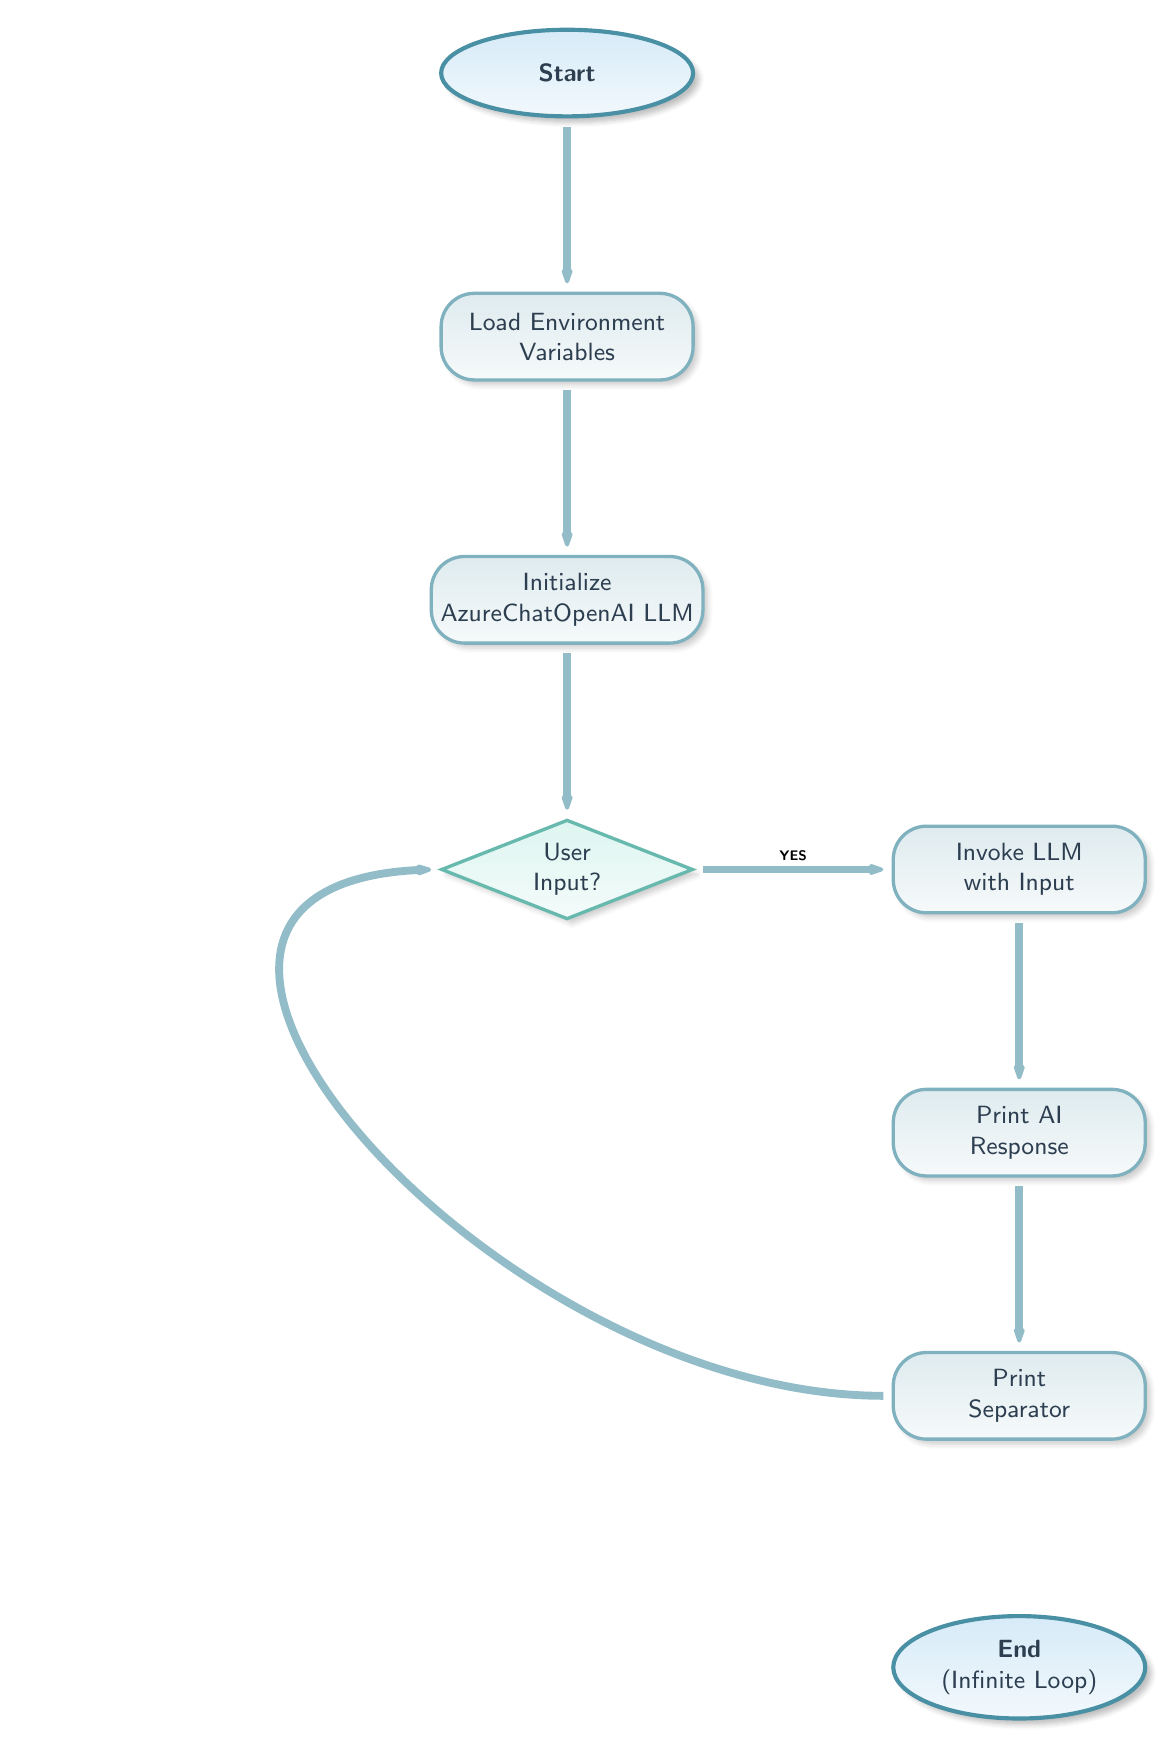
\begin{tikzpicture}[node distance=2.2cm, font=\sffamily\small, every node/.style={align=center}]
    \node (start) [startstop] {\textbf{Start}};
    \node (load) [process, below=of start] {Load Environment\\Variables};
    \node (init) [process, below=of load] {Initialize\\AzureChatOpenAI LLM};
    \node (loop) [decision, below=of init] {User\\Input?};
    \node (invoke) [process, right=2.5cm of loop] {Invoke LLM\\with Input};
    \node (print) [process, below=of invoke] {Print AI\\Response};
    \node (sep) [process, below=of print] {Print\\Separator};
    \node (end) [startstop, below=of sep] {\textbf{End}\\\small (Infinite Loop)};

    \draw [arrow] (start) -- (load);
    \draw [arrow] (load) -- (init);
    \draw [arrow] (init) -- (loop);
    \draw [arrow] (loop) -- node[above, font=\tiny\bfseries, fill=white, inner sep=2pt] {YES} (invoke);
    \draw [arrow] (invoke) -- (print);
    \draw [arrow] (print) -- (sep);
    \draw [arrow] (sep.west) to[out=180, in=180, looseness=1.5] (loop.west);
\end{tikzpicture}
\end{center}
\vspace{1em}

\newpage
\section{Ollama Equivalent Code}
\vspace{0.5em}
\begin{lstlisting}[language=Python]
from langchain_ollama import OllamaLLM

llm = OllamaLLM(model="qwen3:4b", temperature=0.7)

while True:
    input_text = input("Enter your query: ")
    result = llm.invoke(input_text)
    print("AI:", result)
    print("--------------------------------------------------")
\end{lstlisting}

\subsection{Diff Explanation}

\begin{removedcode}
\begin{diffverb}
- from langchain.chat_models import AzureChatOpenAI
- import os
- from dotenv import load_dotenv
- load_dotenv()
- llm = AzureChatOpenAI(
-     openai_api_base=os.getenv("AZURE_OPENAI_API_BASE"),
-     openai_api_version=os.getenv("AZURE_OPENAI_API_VERSION"),
-     openai_api_key=os.getenv("AZURE_OPENAI_API_KEY"),
-     openai_api_version=os.getenv("AZURE_OPENAI_DEPLOYMENT_NAME"),
-     model_name="gpt-4o",
-     temperature=0.7,
- )
\end{diffverb}
\end{removedcode}

\begin{addedcode}
\begin{diffverb}
+ from langchain_ollama import OllamaLLM
+ llm = OllamaLLM(model="qwen3:4b", temperature=0.7)
\end{diffverb}
\end{addedcode}

\begin{modifiedcode}
print("AI:", result.content) -> print("AI:", result)
\end{modifiedcode}

\subsection{Explanation of the Diff}
\begin{itemize}
    \item \textbf{Removed imports and initialization:} The Azure-specific imports and environment variable loading are removed because Ollama runs locally and doesn't require API keys or cloud configuration.
    \item \textbf{Changed LLM initialization:} Switched to OllamaLLM for local model execution, using a specific model name "qwen3:4b" instead of Azure's gpt-4o.
    \item \textbf{Modified print statement:} In Ollama, the result is directly the string, not an object with .content, so no need to access .content.
    \item \textbf{Why:} These changes adapt the code from cloud-based Azure OpenAI to local Ollama deployment, simplifying setup by removing authentication and using local model inference.
\end{itemize}

\newpage
\section{Hugging Face Equivalent Code}
\vspace{0.5em}
\begin{lstlisting}[language=Python]
from transformers import pipeline

pipe = pipeline("text-generation", model="Qwen/Qwen3-0.6B")

while True:
    input_text = input("Enter your query: ")
    result = pipe(input_text, max_length=100, temperature=0.7, num_return_sequences=1)
    print("AI:", result[0]['generated_text'])
    print("--------------------------------------------------")
\end{lstlisting}

\subsection{Diff Explanation}
\vspace{0.5em}

\begin{removedcode}
\begin{diffverb}
- from langchain.chat_models import AzureChatOpenAI
- import os
- from dotenv import load_dotenv
- load_dotenv()
- llm = AzureChatOpenAI(...)
- result = llm.invoke(input_text)
- print("AI:",result.content)
\end{diffverb}
\end{removedcode}

\begin{addedcode}
\begin{diffverb}
+ from transformers import pipeline
+ pipe = pipeline("text-generation", model="Qwen/Qwen3-0.6B")
+ result = pipe(input_text, max_length=100, temperature=0.7,
+              num_return_sequences=1)
+ print("AI:", result[0]['generated_text'])
\end{diffverb}
\end{addedcode}

\subsection{Explanation of the Diff}
\begin{itemize}
    \item \textbf{Removed LangChain and Azure setup:} Replaced with Hugging Face transformers for direct model interaction.
    \item \textbf{Changed to pipeline:} Uses text-generation pipeline with a specific model, adding parameters like max\_length and num\_return\_sequences for generation control.
    \item \textbf{Modified result handling:} The result is a list of dictionaries, accessing the generated text accordingly.
    \item \textbf{Why:} Hugging Face provides a different API focused on transformers models, requiring different initialization and invocation methods, and handles generation parameters explicitly.
\end{itemize}



% ===== CODE2 =====
\newpage
\section{Original Code: code2.py}
\begin{lstlisting}[language=Python]
import os
from dotenv import load_dotenv
from langchain_openai import AzureChatOpenAI

# Load environment variables
load_dotenv()

# Fetch from .env or directly assign as needed
api_key = ""
api_base = "https://chatgpt-key.openai.azure.com/"
deployment_name = "gpt-4o-2"
api_version = "2024-12-01-preview"  # Ensure this is a valid API version

print(f"API Key: {api_key}")

# Initialize the model
llm = AzureChatOpenAI(
    deployment_name=deployment_name,
    api_version=api_version,
    api_key=api_key,
    azure_endpoint=api_base,
    model_name="gpt-4o",
    temperature=0.7,
    max_tokens=100,  # Maximum number of tokens in the response
)


# Use the predict method instead of chat
response = llm.predict("Hello, how are you?")

# Print the response
print(response)
\end{lstlisting}

\subsection{Explanation of the Code}
\begin{itemize}
    \item \textbf{What:} This code initializes an Azure OpenAI model using LangChain and generates a single response to the prompt "Hello, how are you?" using the predict method, then prints the response.
    \item \textbf{Why:} It demonstrates basic setup and single-query interaction with Azure OpenAI via LangChain. The use of predict method shows an alternative to invoke for simple text generation. Environment variables are loaded for security, though here API key is empty (placeholder). This approach is for testing or simple API calls without continuous interaction.
    \item \textbf{How:}
    \begin{itemize}
        \item Load environment variables (though API key is hardcoded empty here).
        \item Print the API key (for debugging).
        \item Initialize AzureChatOpenAI with deployment details, API version, key, endpoint, model name, temperature, and max tokens.
        \item Call predict with a fixed prompt to get a response.
        \item Print the response string.
    \end{itemize}
\end{itemize}

\subsection{Flowchart}
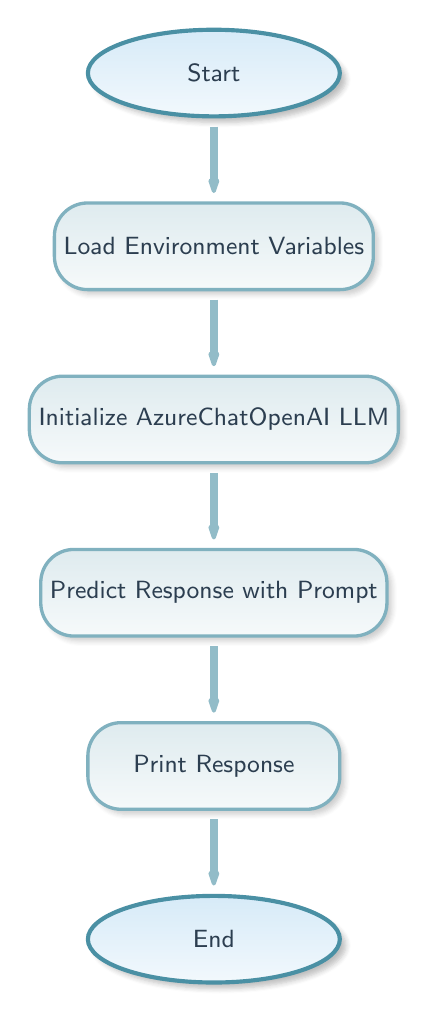
\begin{tikzpicture}[node distance=2.2cm, font=\sffamily\small]
    \node (start) [startstop] {Start};
    \node (load) [process, below of=start] {Load Environment Variables};
    \node (init) [process, below of=load] {Initialize AzureChatOpenAI LLM};
    \node (predict) [process, below of=init] {Predict Response with Prompt};
    \node (print) [process, below of=predict] {Print Response};
    \node (end) [startstop, below of=print] {End};

    \draw [arrow] (start) -- (load);
    \draw [arrow] (load) -- (init);
    \draw [arrow] (init) -- (predict);
    \draw [arrow] (predict) -- (print);
    \draw [arrow] (print) -- (end);
\end{tikzpicture}

\section{Ollama Equivalent Code}
\begin{lstlisting}[language=Python]
from langchain_ollama import OllamaLLM

llm = OllamaLLM(
    model="qwen3:4b",
    temperature=0.7,
    max_tokens=100,
)

response = llm.invoke("Hello, how are you?")

print(response)
\end{lstlisting}

\subsection{Diff Explanation}
\begin{removedcode}
\begin{diffverb}
- import os
- from dotenv import load_dotenv
- from langchain_openai import AzureChatOpenAI
- load_dotenv()
- api_key = ""
- api_base = "https://chatgpt-key.openai.azure.com/"
- deployment_name = "gpt-4o-2"
- api_version = "2024-12-01-preview"
- print(f"API Key: {api_key}")
- llm = AzureChatOpenAI(...)
- response = llm.predict("Hello, how are you?")
\end{diffverb}
\end{removedcode}

\begin{addedcode}
\begin{diffverb}
+ from langchain_ollama import OllamaLLM
+ llm = OllamaLLM(model="qwen3:4b", temperature=0.7, max_tokens=100)
\end{diffverb}
\end{addedcode}

\begin{modifiedcode}
response = llm.invoke("Hello, how are you?")
\end{modifiedcode}


\subsection{Explanation of the Diff}
\begin{itemize}
    \item \textbf{Removed Azure setup:} Eliminated environment loading, API key handling, and Azure-specific parameters since Ollama is local.
    \item \textbf{Changed initialization:} Used OllamaLLM with model name and parameters.
    \item \textbf{Modified invocation:} Switched from predict to invoke, as Ollama uses invoke for generation.
    \item \textbf{Why:} Adapts to Ollama's local execution, removing cloud dependencies and using LangChain's Ollama wrapper for consistency.
\end{itemize}

\section{Hugging Face Equivalent Code}
\begin{lstlisting}[language=Python]
from transformers import pipeline

pipe = pipeline("text-generation", model="Qwen/Qwen3-0.6B")

response = pipe("Hello, how are you?", max_new_tokens=50, temperature=0.7, num_return_sequences=1)

print(response[0]['generated_text'])
\end{lstlisting}

\subsection{Diff Explanation}
\begin{removedcode}
\begin{diffverb}
- import os
- from dotenv import load_dotenv
- from langchain_openai import AzureChatOpenAI
- load_dotenv()
- api_key = ""
- ... (Azure init)
- response = llm.predict("Hello, how are you?")
- print(response)
\end{diffverb}
\end{removedcode}

\begin{addedcode}
\begin{diffverb}
+ from transformers import pipeline
+ pipe = pipeline("text-generation", model="Qwen/Qwen3-0.6B")
+ response = pipe("Hello, how are you?", max_new_tokens=50, temperature=0.7, num_return_sequences=1)
+ print(response[0]['generated_text'])
\end{diffverb}
\end{addedcode}


\subsection{Explanation of the Diff}
\begin{itemize}
    \item \textbf{Removed LangChain and Azure:} Replaced with direct Hugging Face pipeline.
    \item \textbf{Changed to pipeline generation:} Used text-generation pipeline with max\_new\_tokens instead of max\_tokens.
    \item \textbf{Modified output handling:} Accessed the generated text from the result list.
    \item \textbf{Why:} Hugging Face transformers provide a different interface for model loading and generation, focusing on local model execution without LangChain abstraction.
\end{itemize}


% ===== CODE3 =====
\newpage
\section{Original Code: code3.py}
\begin{lstlisting}[language=Python]
#ChatAnthropic - cluade

from langchain_anthropic import ChatAnthropic
from dotenv import load_dotenv
import os
load_dotenv()
llm=ChatAnthropic(temperature=0.7, model="claude-2", anthropic_api_key=os.getenv("ANTHROPIC_API_KEY"))
result=llm.invoke("What is the capital of France?")
print(result)
\end{lstlisting}

\subsection{Explanation of the Code}
\begin{itemize}
    \item \textbf{What:} This code initializes a ChatAnthropic model (Claude) using LangChain and generates a response to the query "What is the capital of France?", then prints the result.
    \item \textbf{Why:} Demonstrates integration with Anthropic's Claude model via LangChain for AI-powered question answering. Uses environment variables for API key security. This approach is for simple, single-turn interactions with proprietary models like Claude.
    \item \textbf{How:}
    \begin{itemize}
        \item Load environment variables from .env file.
        \item Initialize ChatAnthropic with temperature, model name, and API key from env.
        \item Invoke the model with a fixed question.
        \item Print the result object (which contains the response).
    \end{itemize}
\end{itemize}

\subsection{Flowchart}
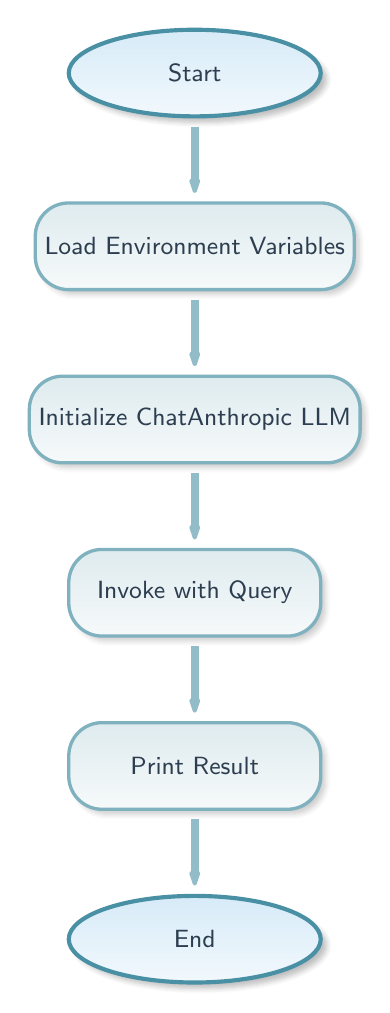
\begin{tikzpicture}[node distance=2.2cm, font=\sffamily\small]
    \node (start) [startstop] {Start};
    \node (load) [process, below of=start] {Load Environment Variables};
    \node (init) [process, below of=load] {Initialize ChatAnthropic LLM};
    \node (invoke) [process, below of=init] {Invoke with Query};
    \node (print) [process, below of=invoke] {Print Result};
    \node (end) [startstop, below of=print] {End};

    \draw [arrow] (start) -- (load);
    \draw [arrow] (load) -- (init);
    \draw [arrow] (init) -- (invoke);
    \draw [arrow] (invoke) -- (print);
    \draw [arrow] (print) -- (end);
\end{tikzpicture}

\section{Ollama Equivalent Code}
\begin{lstlisting}[language=Python]
from langchain_ollama import OllamaLLM

llm = OllamaLLM(model="qwen3:4b", temperature=0.7)

result = llm.invoke("What is the capital of France?")

print(result)
\end{lstlisting}

\subsection{Diff Explanation}
\begin{removedcode}
\begin{diffverb}
- from langchain_anthropic import ChatAnthropic
- from dotenv import load_dotenv
- import os
- load_dotenv()
- llm=ChatAnthropic(temperature=0.7, model="claude-2", anthropic_api_key=os.getenv("ANTHROPIC_API_KEY"))
\end{diffverb}
\end{removedcode}

\begin{addedcode}
\begin{diffverb}
+ from langchain_ollama import OllamaLLM
+ llm = OllamaLLM(model="qwen3:4b", temperature=0.7)
\end{diffverb}
\end{addedcode}


\subsection{Explanation of the Diff}
\begin{itemize}
    \item \textbf{Removed Anthropic setup:} Eliminated API key loading and ChatAnthropic initialization.
    \item \textbf{Changed to Ollama:} Used OllamaLLM for local execution.
    \item \textbf{Why:} Switches from cloud-based Anthropic API to local Ollama model, removing authentication requirements.
\end{itemize}

\section{Hugging Face Equivalent Code}
\begin{lstlisting}[language=Python]
from transformers import pipeline

pipe = pipeline("text-generation", model="Qwen/Qwen3-0.6B")

result = pipe("What is the capital of France?", max_new_tokens=50, temperature=0.7, num_return_sequences=1)

print(result[0]['generated_text'])
\end{lstlisting}

\subsection{Diff Explanation}
\begin{removedcode}
\begin{diffverb}
- from langchain_anthropic import ChatAnthropic
- from dotenv import load_dotenv
- import os
- load_dotenv()
- llm=ChatAnthropic(...)
- result=llm.invoke("What is the capital of France?")
- print(result)
\end{diffverb}
\end{removedcode}

\begin{addedcode}
\begin{diffverb}
+ from transformers import pipeline
+ pipe = pipeline("text-generation", model="Qwen/Qwen3-0.6B")
+ result = pipe("What is the capital of France?", max_new_tokens=50, temperature=0.7, num_return_sequences=1)
+ print(result[0]['generated_text'])
\end{diffverb}
\end{addedcode}


\subsection{Explanation of the Diff}
\begin{itemize}
    \item \textbf{Removed LangChain Anthropic:} Replaced with Hugging Face pipeline.
    \item \textbf{Changed invocation and output:} Used pipeline generate method and accessed text from result.
    \item \textbf{Why:} Adapts to Hugging Face's direct model interface for text generation.
\end{itemize}


% ===== CODE4 =====
\newpage
\section{Original Code: code4.py}
\begin{lstlisting}[language=Python]
from langchain_google_genai import ChatGoogleGenAI
from dotenv import load_dotenv
import os
load_dotenv()

llm=ChatGoogleGenAI(temperature=0.7, model="gemini-1.5-pro", google_api_key=os.getenv("GOOGLE_API_KEY"))


result=llm.invoke("What is the capital of France?")
print(result)
\end{lstlisting}

\subsection{Explanation of the Code}
\begin{itemize}
    \item \textbf{What:} This code initializes a ChatGoogleGenAI model (Gemini) using LangChain and generates a response to "What is the capital of France?", then prints it.
    \item \textbf{Why:} Shows integration with Google's Gemini model via LangChain for AI responses. Uses env vars for API key. Suitable for single queries to Google's AI.
    \item \textbf{How:}
    \begin{itemize}
        \item Load env vars.
        \item Init ChatGoogleGenAI with temp, model, API key.
        \item Invoke with query.
        \item Print result.
    \end{itemize}
\end{itemize}

\subsection{Flowchart}
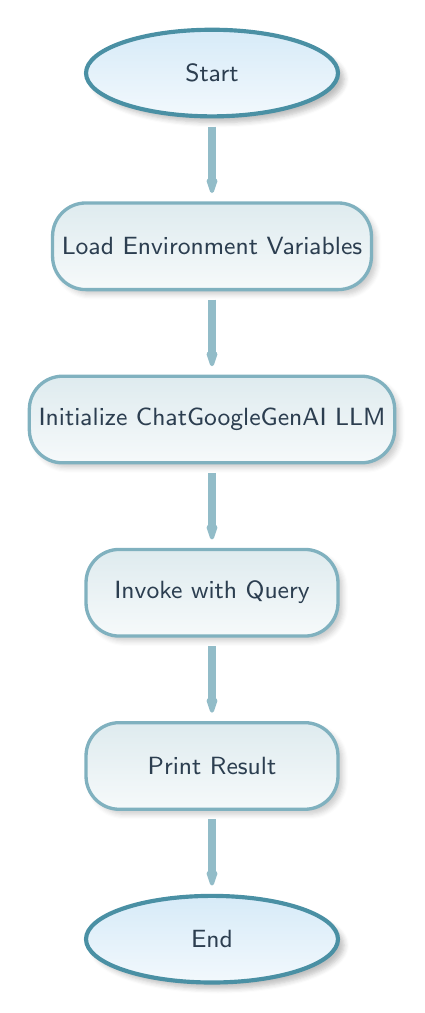
\begin{tikzpicture}[node distance=2.2cm, font=\sffamily\small]
    \node (start) [startstop] {Start};
    \node (load) [process, below of=start] {Load Environment Variables};
    \node (init) [process, below of=load] {Initialize ChatGoogleGenAI LLM};
    \node (invoke) [process, below of=init] {Invoke with Query};
    \node (print) [process, below of=invoke] {Print Result};
    \node (end) [startstop, below of=print] {End};

    \draw [arrow] (start) -- (load);
    \draw [arrow] (load) -- (init);
    \draw [arrow] (init) -- (invoke);
    \draw [arrow] (invoke) -- (print);
    \draw [arrow] (print) -- (end);
\end{tikzpicture}

\section{Ollama Equivalent Code}
\begin{lstlisting}[language=Python]
from langchain_ollama import OllamaLLM

llm = OllamaLLM(model="qwen3:4b", temperature=0.7)

result = llm.invoke("What is the capital of France?")

print(result)
\end{lstlisting}

\subsection{Diff Explanation}
\begin{removedcode}
\begin{diffverb}
- from langchain_google_genai import ChatGoogleGenAI
- from dotenv import load_dotenv
- import os
- load_dotenv()
- llm=ChatGoogleGenAI(temperature=0.7, model="gemini-1.5-pro", google_api_key=os.getenv("GOOGLE_API_KEY"))
\end{diffverb}
\end{removedcode}

\begin{addedcode}
\begin{diffverb}
+ from langchain_ollama import OllamaLLM
+ llm = OllamaLLM(model="qwen3:4b", temperature=0.7)
\end{diffverb}
\end{addedcode}


\subsection{Explanation of the Diff}
\begin{itemize}
    \item \textbf{Removed Google setup:} Eliminated API key and ChatGoogleGenAI.
    \item \textbf{Changed to Ollama:} Local model execution.
    \item \textbf{Why:} From cloud Google API to local Ollama.
\end{itemize}

\section{Hugging Face Equivalent Code}
\begin{lstlisting}[language=Python]
from transformers import pipeline

pipe = pipeline("text-generation", model="Qwen/Qwen3-0.6B")

result = pipe("What is the capital of France?", max_new_tokens=50, temperature=0.7, num_return_sequences=1)

print(result[0]['generated_text'])
\end{lstlisting}

\subsection{Diff Explanation}
\begin{removedcode}
\begin{diffverb}
- from langchain_google_genai import ChatGoogleGenAI
- ...
- result=llm.invoke("What is the capital of France?")
- print(result)
\end{diffverb}
\end{removedcode}

\begin{addedcode}
\begin{diffverb}
+ from transformers import pipeline
+ pipe = pipeline("text-generation", model="Qwen/Qwen3-0.6B")
+ result = pipe("What is the capital of France?", max_new_tokens=50, temperature=0.7, num_return_sequences=1)
+ print(result[0]['generated_text'])
\end{diffverb}
\end{addedcode}


\subsection{Explanation of the Diff}
\begin{itemize}
    \item \textbf{Removed LangChain Google:} To Hugging Face pipeline.
    \item \textbf{Changed invocation:} Pipeline generate.
    \item \textbf{Why:} Direct transformers usage.
\end{itemize}


% ===== CODE5 =====
\newpage
\section{Original Code: code5.py}
\begin{lstlisting}[language=Python]
from langchain_openai import ChatOpenAI

from langchain_google_genai import ChatGoogleGenAI

from langchain_anthropic import ChatAnthropic

from dotenv import load_dotenv
import os


llm1=ChatOpenAI(model="gpt-3.5-turbo",temperature=0.5,openai_api_key=os.getenv("OPENAI_API_KEY"))
llm2=ChatGoogleGenAI(temperature=0.7, model="gemini-1.5-pro", google_api_key=os.getenv("GOOGLE_API_KEY"))
llm3=ChatAnthropic(temperature=0.7, model="claude-2", anthropic_api_key=os.getenv("ANTHROPIC_API_KEY"))

result1=llm1.invoke("Opinion on Pakistan?")
result2=llm2.invoke("Opinion on Pakistan?")
result3=llm3.invoke("Opinion on Pakistan?")

print("OpenAI result: ",result1)
print("Google result: ",result2)
print("Anthropic result: ",result3)
\end{lstlisting}

\subsection{Explanation of the Code}
\begin{itemize}
    \item \textbf{What:} This code initializes three different LLM models (OpenAI GPT-3.5, Google Gemini, Anthropic Claude) using LangChain and generates responses to the same query "Opinion on Pakistan?" from each, then prints them labeled by provider.
    \item \textbf{Why:} Demonstrates comparing outputs from multiple AI providers for the same prompt, highlighting differences in responses. Uses env vars for API keys. This is useful for evaluating model performance or biases across platforms.
    \item \textbf{How:}
    \begin{itemize}
        \item Load env vars.
        \item Initialize three LLMs with different providers, models, and temps.
        \item Invoke each with the same query.
        \item Print results with labels.
    \end{itemize}
\end{itemize}

\subsection{Flowchart}
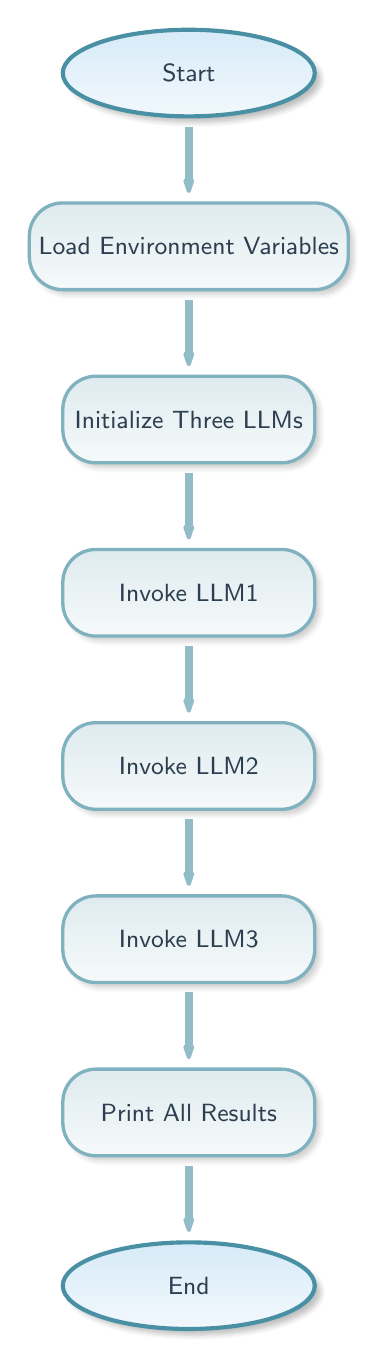
\begin{tikzpicture}[node distance=2.2cm, font=\sffamily\small]
    \node (start) [startstop] {Start};
    \node (load) [process, below of=start] {Load Environment Variables};
    \node (init) [process, below of=load] {Initialize Three LLMs};
    \node (invoke1) [process, below of=init] {Invoke LLM1};
    \node (invoke2) [process, below of=invoke1] {Invoke LLM2};
    \node (invoke3) [process, below of=invoke2] {Invoke LLM3};
    \node (print) [process, below of=invoke3] {Print All Results};
    \node (end) [startstop, below of=print] {End};

    \draw [arrow] (start) -- (load);
    \draw [arrow] (load) -- (init);
    \draw [arrow] (init) -- (invoke1);
    \draw [arrow] (invoke1) -- (invoke2);
    \draw [arrow] (invoke2) -- (invoke3);
    \draw [arrow] (invoke3) -- (print);
    \draw [arrow] (print) -- (end);
\end{tikzpicture}

\section{Ollama Equivalent Code}
\begin{lstlisting}[language=Python]
from langchain_ollama import OllamaLLM

llm1 = OllamaLLM(model="qwen3:4b", temperature=0.5)
llm2 = OllamaLLM(model="qwen3:4b", temperature=0.7)  # Change model name to ones installed for better experience
llm3 = OllamaLLM(model="qwen3:4b", temperature=0.7)  # Change model name to ones installed for better experience

result1 = llm1.invoke("Opinion on Pakistan?")
result2 = llm2.invoke("Opinion on Pakistan?")
result3 = llm3.invoke("Opinion on Pakistan?")

print("OpenAI result: ", result1)
print("Google result: ", result2)
print("Anthropic result: ", result3)
\end{lstlisting}

\subsection{Diff Explanation}
\begin{removedcode}
\begin{diffverb}
- from langchain_openai import ChatOpenAI
- from langchain_google_genai import ChatGoogleGenAI
- from langchain_anthropic import ChatAnthropic
- from dotenv import load_dotenv
- import os
- llm1=ChatOpenAI(model="gpt-3.5-turbo",temperature=0.5,openai_api_key=os.getenv("OPENAI_API_KEY"))
- llm2=ChatGoogleGenAI(temperature=0.7, model="gemini-1.5-pro", google_api_key=os.getenv("GOOGLE_API_KEY"))
- llm3=ChatAnthropic(temperature=0.7, model="claude-2", anthropic_api_key=os.getenv("ANTHROPIC_API_KEY"))
\end{diffverb}
\end{removedcode}

\begin{addedcode}
\begin{diffverb}
+ from langchain_ollama import OllamaLLM
+ llm1 = OllamaLLM(model="qwen3:4b", temperature=0.5)
+ llm2 = OllamaLLM(model="qwen3:4b", temperature=0.7)
+ llm3 = OllamaLLM(model="qwen3:4b", temperature=0.7)
\end{diffverb}
\end{addedcode}


\subsection{Explanation of the Diff}
\begin{itemize}
    \item \textbf{Removed multiple provider setups:} Eliminated API keys and different LangChain imports.
    \item \textbf{Changed to multiple Ollama instances:} Used same model with varying temperatures for comparison.
    \item \textbf{Why:} Adapts to local Ollama, simulating multi-model comparison with different configs instead of different providers.
\end{itemize}

\section{Hugging Face Equivalent Code}
\begin{lstlisting}[language=Python]
from transformers import pipeline

pipe1 = pipeline("text-generation", model="Qwen/Qwen3-0.6B")
pipe2 = pipeline("text-generation", model="Qwen/Qwen3-0.6B")  # Change model name to ones installed for better experience
pipe3 = pipeline("text-generation", model="Qwen/Qwen3-0.6B")  # Change model name to ones installed for better experience

result1 = pipe1("Opinion on Pakistan?", max_new_tokens=50, temperature=0.5, num_return_sequences=1)
result2 = pipe2("Opinion on Pakistan?", max_new_tokens=50, temperature=0.7, num_return_sequences=1)
result3 = pipe3("Opinion on Pakistan?", max_new_tokens=50, temperature=0.7, num_return_sequences=1)

print("OpenAI result: ", result1[0]['generated_text'])
print("Google result: ", result2[0]['generated_text'])
print("Anthropic result: ", result3[0]['generated_text'])
\end{lstlisting}

\subsection{Diff Explanation}
\begin{removedcode}
\begin{diffverb}
- from langchain_openai import ChatOpenAI
- ...
- llm1=...
- llm2=...
- llm3=...
- result1=llm1.invoke("Opinion on Pakistan?")
- result2=llm2.invoke("Opinion on Pakistan?")
- result3=llm3.invoke("Opinion on Pakistan?")
- print("OpenAI result: ",result1)
- print("Google result: ",result2)
- print("Anthropic result: ",result3)
\end{diffverb}
\end{removedcode}

\begin{addedcode}
\begin{diffverb}
+ from transformers import pipeline
+ pipe1 = pipeline("text-generation", model="Qwen/Qwen3-0.6B")
+ pipe2 = pipeline("text-generation", model="Qwen/Qwen3-0.6B")
+ pipe3 = pipeline("text-generation", model="Qwen/Qwen3-0.6B")
+ result1 = pipe1("Opinion on Pakistan?", max_new_tokens=50, temperature=0.5, num_return_sequences=1)
+ result2 = pipe2("Opinion on Pakistan?", max_new_tokens=50, temperature=0.7, num_return_sequences=1)
+ result3 = pipe3("Opinion on Pakistan?", max_new_tokens=50, temperature=0.7, num_return_sequences=1)
+ print("OpenAI result: ", result1[0]['generated_text'])
+ print("Google result: ", result2[0]['generated_text'])
+ print("Anthropic result: ", result3[0]['generated_text'])
\end{diffverb}
\end{addedcode}


\subsection{Explanation of the Diff}
\begin{itemize}
    \item \textbf{Removed LangChain multi-provider:} Replaced with multiple Hugging Face pipelines.
    \item \textbf{Changed invocation and output:} Used pipeline generate and accessed text.
    \item \textbf{Why:} Uses direct transformers for local multi-instance comparison.
\end{itemize}


% ===== CODE6 =====
\newpage
\section{Original Code: code6.py}
\begin{lstlisting}[language=Python]
from langchain.prompts import PromptTemplate

prompt=PromptTemplate(
    input_variables=["input"],
    template="What is the capital of {input}?",
)

print(prompt.format(input="China"))
\end{lstlisting}

\subsection{Explanation of the Code}
\begin{itemize}
    \item \textbf{What:} This code defines a PromptTemplate with a placeholder for input, formats it with "China", and prints the resulting prompt string.
    \item \textbf{Why:} Demonstrates LangChain's PromptTemplate for dynamic prompt creation. Useful for reusable prompts with variables. Here, it just formats and prints without invoking an LLM.
    \item \textbf{How:}
    \begin{itemize}
        \item Import PromptTemplate.
        \item Create template with input\_variables and template string.
        \item Format with specific input.
        \item Print the formatted string.
    \end{itemize}
\end{itemize}

\subsection{Flowchart}
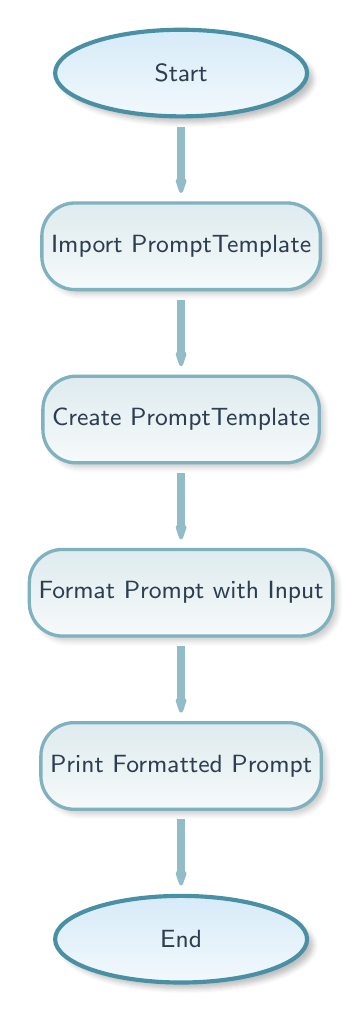
\begin{tikzpicture}[node distance=2.2cm, font=\sffamily\small]
    \node (start) [startstop] {Start};
    \node (import) [process, below of=start] {Import PromptTemplate};
    \node (create) [process, below of=import] {Create PromptTemplate};
    \node (format) [process, below of=create] {Format Prompt with Input};
    \node (print) [process, below of=format] {Print Formatted Prompt};
    \node (end) [startstop, below of=print] {End};

    \draw [arrow] (start) -- (import);
    \draw [arrow] (import) -- (create);
    \draw [arrow] (create) -- (format);
    \draw [arrow] (format) -- (print);
    \draw [arrow] (print) -- (end);
\end{tikzpicture}

\section{Ollama Equivalent Code}
\begin{lstlisting}[language=Python]
from langchain_core.prompts import PromptTemplate
from langchain_ollama import OllamaLLM

# Initialize the LLM with Ollama
llm = OllamaLLM(model="qwen3:4b")

prompt = PromptTemplate(
    input_variables=["input"],
    template="What is the capital of {input}?",
)

# Create a chain
chain = prompt | llm

# Invoke the chain
result = chain.invoke({"input": "China"})
print(result)
\end{lstlisting}

\subsection{Diff Explanation}
\begin{removedcode}
\begin{diffverb}
- from langchain.prompts import PromptTemplate
- prompt=PromptTemplate(...)
- print(prompt.format(input="China"))
\end{diffverb}
\end{removedcode}

\begin{addedcode}
\begin{diffverb}
+ from langchain_core.prompts import PromptTemplate
+ from langchain_ollama import OllamaLLM
+ llm = OllamaLLM(model="qwen3:4b")
+ chain = prompt | llm
+ result = chain.invoke({"input": "China"})
+ print(result)
\end{diffverb}
\end{addedcode}


\subsection{Explanation of the Diff}
\begin{itemize}
    \item \textbf{Added LLM and chaining:} Introduced OllamaLLM and chain composition with | operator.
    \item \textbf{Changed invocation:} From formatting only to invoking the chain with dict input.
    \item \textbf{Why:} Extends to actual LLM invocation using LangChain's chaining for prompt + model.
\end{itemize}

\section{Hugging Face Equivalent Code}
\begin{lstlisting}[language=Python]
from transformers import pipeline

# Initialize the pipeline with Qwen model
pipe = pipeline("text-generation", model="Qwen/Qwen3-0.6B")

# Format the prompt
prompt = "What is the capital of China?"

# Generate text
result = pipe(prompt, max_new_tokens=50)
print(result[0]['generated_text'])
\end{lstlisting}

\subsection{Diff Explanation}
\begin{removedcode}
\begin{diffverb}
- from langchain.prompts import PromptTemplate
- prompt=PromptTemplate(...)
- print(prompt.format(input="China"))
\end{diffverb}
\end{removedcode}

\begin{addedcode}
\begin{diffverb}
+ from transformers import pipeline
+ pipe = pipeline("text-generation", model="Qwen/Qwen3-0.6B")
+ prompt = "What is the capital of China?"
+ result = pipe(prompt, max_new_tokens=50)
+ print(result[0]['generated_text'])
\end{diffverb}
\end{addedcode}


\subsection{Explanation of the Diff}
\begin{itemize}
    \item \textbf{Removed PromptTemplate:} Manual string formatting.
    \item \textbf{Added pipeline generation:} Direct text generation with pipeline.
    \item \textbf{Why:} Hugging Face doesn't use LangChain templates, so manual prompt creation and pipeline invocation.
\end{itemize}


% ===== CODE7 =====
\newpage
\section{Original Code: code7.py}
\begin{lstlisting}[language=Python]
from langchain.prompts import PromptTemplate

from langchain.chat_models import AzureChatOpenAI

from langchain.chains import LLMChain
from dotenv import load_dotenv
import os
load_dotenv()
# Fetch from .env
api_key = os.getenv("AZURE_OPENAI_API_KEY")
api_base = os.getenv("AZURE_OPENAI_ENDPOINT")
deployment_name = os.getenv("AZURE_OPENAI_DEPLOYMENT_NAME")
api_version = os.getenv("AZURE_OPENAI_API_VERSION")
llm=AzureChatOpenAI(
    deployment_name=deployment_name,
    api_version=api_version,
    api_key=api_key,
    azure_endpoint=api_base,
    model_name="gpt-4",
    temperature=0.9,
    top_p=0.9,
    max_tokens=100,
# Maximum number of tokens in the response
)
promt=PromptTemplate(
    input_variables=["country"],
    template="what your opinion on this country {country}?",
)
chain=LLMChain(llm=llm,prompt=promt)
result=chain.invoke({"country":"India"})
print(result['text'])
\end{lstlisting}

\subsection{Explanation of the Code}
\begin{itemize}
    \item \textbf{What:} This code creates a prompt template, initializes an Azure OpenAI LLM, combines them into an LLMChain, invokes the chain with "India" as input, and prints the generated text.
    \item \textbf{Why:} Demonstrates LangChain's chaining mechanism to combine prompts and LLMs for dynamic query generation. Uses Azure for cloud AI, with parameters like temperature and top\_p for response control.
    \item \textbf{How:}
    \begin{itemize}
        \item Load env vars for Azure credentials.
        \item Init AzureChatOpenAI with params.
        \item Create PromptTemplate.
        \item Create LLMChain with llm and prompt.
        \item Invoke chain with dict input.
        \item Print result['text'].
    \end{itemize}
\end{itemize}

\subsection{Flowchart}
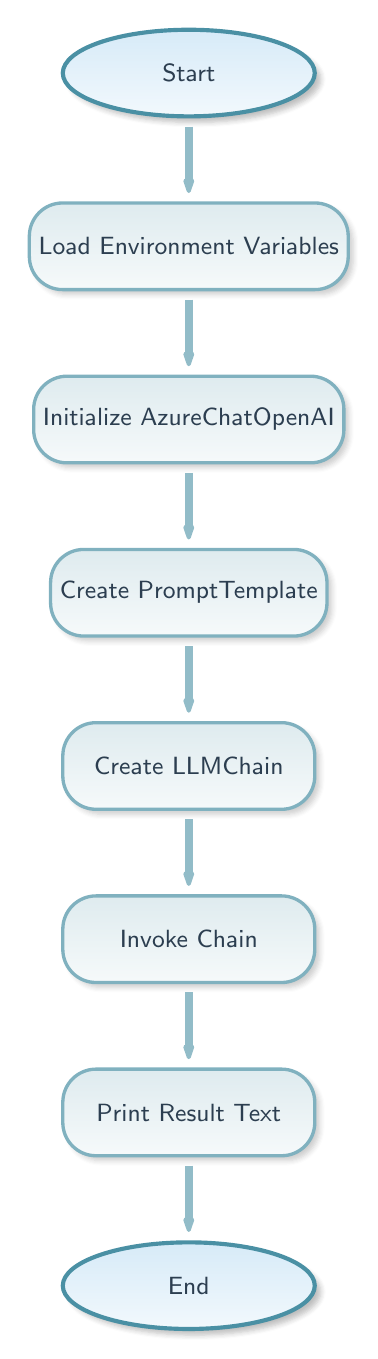
\begin{tikzpicture}[node distance=2.2cm, font=\sffamily\small]
    \node (start) [startstop] {Start};
    \node (load) [process, below of=start] {Load Environment Variables};
    \node (init_llm) [process, below of=load] {Initialize AzureChatOpenAI};
    \node (create_prompt) [process, below of=init_llm] {Create PromptTemplate};
    \node (create_chain) [process, below of=create_prompt] {Create LLMChain};
    \node (invoke) [process, below of=create_chain] {Invoke Chain};
    \node (print) [process, below of=invoke] {Print Result Text};
    \node (end) [startstop, below of=print] {End};

    \draw [arrow] (start) -- (load);
    \draw [arrow] (load) -- (init_llm);
    \draw [arrow] (init_llm) -- (create_prompt);
    \draw [arrow] (create_prompt) -- (create_chain);
    \draw [arrow] (create_chain) -- (invoke);
    \draw [arrow] (invoke) -- (print);
    \draw [arrow] (print) -- (end);
\end{tikzpicture}

\section{Ollama Equivalent Code}
\begin{lstlisting}[language=Python]
from langchain_core.prompts import PromptTemplate
from langchain_ollama import OllamaLLM

# Initialize the LLM with Ollama
llm = OllamaLLM(model="qwen3:4b", temperature=0.9)

prompt = PromptTemplate(
    input_variables=["country"],
    template="what your opinion on this country {country}?",
)

# Create a chain
chain = prompt | llm

# Invoke the chain
result = chain.invoke({"country": "India"})
print(result)
\end{lstlisting}

\subsection{Diff Explanation}
\begin{removedcode}
\begin{diffverb}
- from langchain.prompts import PromptTemplate
- from langchain.chat_models import AzureChatOpenAI
- from langchain.chains import LLMChain
- from dotenv import load_dotenv
- import os
- load_dotenv()
- api_key = os.getenv("AZURE_OPENAI_API_KEY")
- ... (Azure init)
- promt=PromptTemplate(...)
- chain=LLMChain(llm=llm,prompt=promt)
- result=chain.invoke({"country":"India"})
- print(result['text'])
\end{diffverb}
\end{removedcode}

\begin{addedcode}
\begin{diffverb}
+ from langchain_core.prompts import PromptTemplate
+ from langchain_ollama import OllamaLLM
+ llm = OllamaLLM(model="qwen3:4b", temperature=0.9)
+ prompt = PromptTemplate(...)
+ chain = prompt | llm
+ result = chain.invoke({"country": "India"})
+ print(result)
\end{diffverb}
\end{addedcode}


\subsection{Explanation of the Diff}
\begin{itemize}
    \item \textbf{Removed Azure setup and old LLMChain:} Eliminated env loading and AzureChatOpenAI.
    \item \textbf{Changed to modern chaining:} Used | operator instead of LLMChain class.
    \item \textbf{Simplified result access:} Direct print of result instead of result['text'].
    \item \textbf{Why:} Updates to newer LangChain syntax and adapts to Ollama local model.
\end{itemize}

\section{Hugging Face Equivalent Code}
\begin{lstlisting}[language=Python]
from transformers import pipeline

# Initialize the pipeline with Qwen model
pipe = pipeline("text-generation", model="Qwen/Qwen3-0.6B")

# Format the prompt
prompt = "what your opinion on this country India?"

# Generate text
result = pipe(prompt, max_new_tokens=100, temperature=0.9, top_p=0.9)
print(result[0]['generated_text'])
\end{lstlisting}

\subsection{Diff Explanation}
\begin{removedcode}
\begin{diffverb}
- from langchain.prompts import PromptTemplate
- ... (Azure and chain setup)
- result=chain.invoke({"country":"India"})
- print(result['text'])
\end{diffverb}
\end{removedcode}

\begin{addedcode}
\begin{diffverb}
+ from transformers import pipeline
+ pipe = pipeline("text-generation", model="Qwen/Qwen3-0.6B")
+ prompt = "what your opinion on this country India?"
+ result = pipe(prompt, max_new_tokens=100, temperature=0.9, top_p=0.9)
+ print(result[0]['generated_text'])
\end{diffverb}
\end{addedcode}


\subsection{Explanation of the Diff}
\begin{itemize}
    \item \textbf{Removed LangChain components:} No templates or chains.
    \item \textbf{Manual prompt and pipeline:} Direct string prompt and generation.
    \item \textbf{Why:} Hugging Face focuses on direct model interaction without LangChain abstractions.
\end{itemize}


% ===== CODE8 =====
\newpage
\section{Original Code: code8.py}
\begin{lstlisting}[language=Python]
from langchain.chat_models import AzureChatOpenAI
from langchain.prompts import FewShotPromptTemplate, PromptTemplate
from dotenv import load_dotenv
from langchain.chains import LLMChain
import os
load_dotenv()

api_key = os.getenv("AZURE_OPENAI_API_KEY")
api_base = os.getenv("AZURE_OPENAI_ENDPOINT")
deployment_name = os.getenv("AZURE_OPENAI_DEPLOYMENT_NAME")
api_version = os.getenv("AZURE_OPENAI_API_VERSION")

llm=AzureChatOpenAI(
    deployment_name=deployment_name,
    api_version=api_version,
    api_key=api_key,
    azure_endpoint=api_base,
    model_name="gpt-4",
    temperature=0.9,
    top_p=0.9,
    max_tokens=100,
# Maximum number of tokens in the response
)
examples = [
{"question": "What is the capital of France?", "answer": "The capital of France is Paris."},
{"question": "What is the capital of Germany?", "answer": "The capital of Germany is Berlin."},
{"question": "What is the capital of Italy?", "answer": "The capital of Italy is Rome."},
]

examples_prompt = PromptTemplate(
    input_variables=["question", "answer"],
    template="Question: {question}\nAnswer: {answer}",

)

few_shot_prompt = FewShotPromptTemplate(
    examples=examples,
    examples_prompt=examples_prompt,
    input_variables=["question"],
    suffix="Answer:",
    prefix="You are a helpful assistant. Answer the following question.",
)

formatted_prompt = few_shot_prompt.format(question="What is the capital of Spain?")
print(formatted_prompt)

llmchain=LLMChain(
    llm=llm,
    prompt=few_shot_prompt,
)
result=llmchain.invoke({"question":"What is the capital of Spain?"})
print(formatted_prompt)
print(result['text'])
\end{lstlisting}

\subsection{Explanation of the Code}
\begin{itemize}
    \item \textbf{What:} This code sets up a few-shot prompt template with example Q\&A pairs, formats it for a new question, prints the formatted prompt, then uses an LLMChain with Azure OpenAI to generate and print the response.
    \item \textbf{Why:} Demonstrates few-shot learning by providing examples in the prompt to guide the model's response. Useful for tasks requiring specific formats or reasoning patterns. Uses Azure for scalable AI.
    \item \textbf{How:}
    \begin{itemize}
        \item Load env vars.
        \item Init AzureChatOpenAI.
        \item Define examples list.
        \item Create examples\_prompt template.
        \item Create FewShotPromptTemplate with examples, prefix, suffix.
        \item Format the prompt with new question and print.
        \item Create LLMChain and invoke with question.
        \item Print formatted prompt again and result['text'].
    \end{itemize}
\end{itemize}

\subsection{Flowchart}
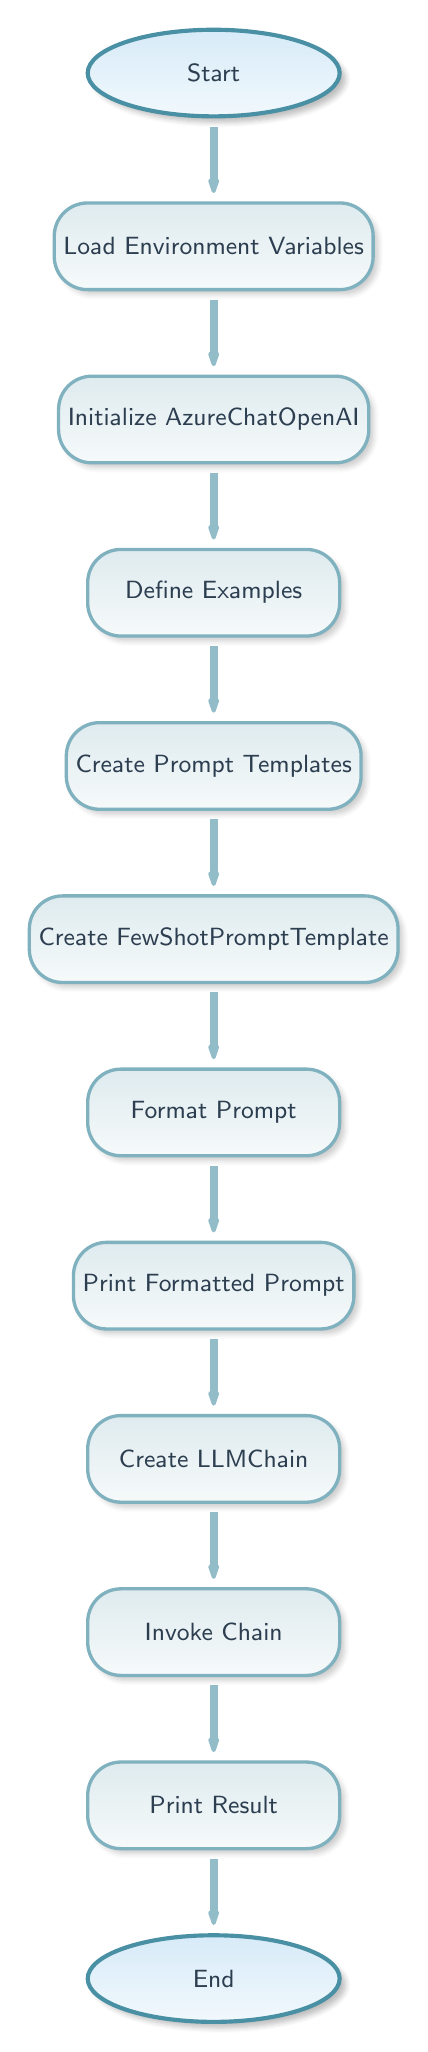
\begin{tikzpicture}[node distance=2.2cm, font=\sffamily\small]
    \node (start) [startstop] {Start};
    \node (load) [process, below of=start] {Load Environment Variables};
    \node (init_llm) [process, below of=load] {Initialize AzureChatOpenAI};
    \node (define_examples) [process, below of=init_llm] {Define Examples};
    \node (create_templates) [process, below of=define_examples] {Create Prompt Templates};
    \node (create_fewshot) [process, below of=create_templates] {Create FewShotPromptTemplate};
    \node (format) [process, below of=create_fewshot] {Format Prompt};
    \node (print_format) [process, below of=format] {Print Formatted Prompt};
    \node (create_chain) [process, below of=print_format] {Create LLMChain};
    \node (invoke) [process, below of=create_chain] {Invoke Chain};
    \node (print_result) [process, below of=invoke] {Print Result};
    \node (end) [startstop, below of=print_result] {End};

    \draw [arrow] (start) -- (load);
    \draw [arrow] (load) -- (init_llm);
    \draw [arrow] (init_llm) -- (define_examples);
    \draw [arrow] (define_examples) -- (create_templates);
    \draw [arrow] (create_templates) -- (create_fewshot);
    \draw [arrow] (create_fewshot) -- (format);
    \draw [arrow] (format) -- (print_format);
    \draw [arrow] (print_format) -- (create_chain);
    \draw [arrow] (create_chain) -- (invoke);
    \draw [arrow] (invoke) -- (print_result);
    \draw [arrow] (print_result) -- (end);
\end{tikzpicture}

\section{Ollama Equivalent Code}
\begin{lstlisting}[language=Python]
from langchain_core.prompts import FewShotPromptTemplate, PromptTemplate
from langchain_ollama import OllamaLLM

# Initialize the LLM with Ollama
llm = OllamaLLM(model="qwen3:4b", temperature=0.9)

examples = [
    {"question": "What is the capital of France?", "answer": "The capital of France is Paris."},
    {"question": "What is the capital of Germany?", "answer": "The capital of Germany is Berlin."},
    {"question": "What is the capital of Italy?", "answer": "The capital of Italy is Rome."},
]

examples_prompt = PromptTemplate(
    input_variables=["question", "answer"],
    template="Question: {question}\nAnswer: {answer}",
)

few_shot_prompt = FewShotPromptTemplate(
    examples=examples,
    example_prompt=examples_prompt,
    input_variables=["question"],
    suffix="Answer:",
    prefix="You are a helpful assistant. Answer the following question.",
)

# Create a chain
chain = few_shot_prompt | llm

# Invoke the chain
result = chain.invoke({"question": "What is the capital of Spain?"})
print(result)
\end{lstlisting}

\subsection{Diff Explanation}
\begin{removedcode}
\begin{diffverb}
- from langchain.chat_models import AzureChatOpenAI
- from langchain.prompts import FewShotPromptTemplate, PromptTemplate
- from dotenv import load_dotenv
- from langchain.chains import LLMChain
- import os
- load_dotenv()
- api_key = ... (Azure setup)
- llm=AzureChatOpenAI(...)
- formatted_prompt = few_shot_prompt.format(question="What is the capital of Spain?")
- print(formatted_prompt)
- llmchain=LLMChain(llm=llm, prompt=few_shot_prompt)
- result=llmchain.invoke({"question":"What is the capital of Spain?"})
- print(formatted_prompt)
- print(result['text'])
\end{diffverb}
\end{removedcode}

\begin{addedcode}
\begin{diffverb}
+ from langchain_core.prompts import FewShotPromptTemplate, PromptTemplate
+ from langchain_ollama import OllamaLLM
+ llm = OllamaLLM(model="qwen3:4b", temperature=0.9)
+ chain = few_shot_prompt | llm
+ result = chain.invoke({"question": "What is the capital of Spain?"})
+ print(result)
\end{diffverb}
\end{addedcode}


\subsection{Explanation of the Diff}
\begin{itemize}
    \item \textbf{Removed Azure and old imports:} Eliminated cloud setup.
    \item \textbf{Updated to modern LangChain:} Used langchain\_core and | chaining.
    \item \textbf{Simplified output:} Removed duplicate prints and direct result printing.
    \item \textbf{Why:} Adapts few-shot prompting to Ollama with updated syntax.
\end{itemize}

\section{Hugging Face Equivalent Code}
\begin{lstlisting}[language=Python]
from transformers import pipeline

# Initialize the pipeline with Qwen model
pipe = pipeline("text-generation", model="Qwen/Qwen3-0.6B")

# Build the few-shot prompt manually
examples = [
    {"question": "What is the capital of France?", "answer": "The capital of France is Paris."},
    {"question": "What is the capital of Germany?", "answer": "The capital of Germany is Berlin."},
    {"question": "What is the capital of Italy?", "answer": "The capital of Italy is Rome."},
]

prompt = "You are a helpful assistant. Answer the following question.\n"
for ex in examples:
    prompt += f"Question: {ex['question']}\nAnswer: {ex['answer']}\n"
prompt += "Question: What is the capital of Spain?\nAnswer:"

# Generate text
result = pipe(prompt, max_new_tokens=100, temperature=0.9, top_p=0.9)
print(result[0]['generated_text'])
\end{lstlisting}

\subsection{Diff Explanation}
\begin{removedcode}
\begin{diffverb}
- from langchain.chat_models import AzureChatOpenAI
- ... (all LangChain setup)
- formatted_prompt = ...
- print(formatted_prompt)
- llmchain=...
- result=...
- print(...)
\end{diffverb}
\end{removedcode}

\begin{addedcode}
\begin{diffverb}
+ from transformers import pipeline
+ pipe = pipeline("text-generation", model="Qwen/Qwen3-0.6B")
+ prompt = "You are a helpful assistant. Answer the following question.\n"
+ for ex in examples:
+     prompt += f"Question: {ex['question']}
Answer: {ex['answer']}
"
+ prompt += "Question: What is the capital of Spain?\nAnswer:"
+ result = pipe(prompt, max_new_tokens=100, temperature=0.9, top_p=0.9)
+ print(result[0]['generated_text'])
\end{diffverb}
\end{addedcode}


\subsection{Explanation of the Diff}
\begin{itemize}
    \item \textbf{Removed LangChain abstractions:} No templates or chains.
    \item \textbf{Manual prompt construction:} Built the few-shot prompt as a string.
    \item \textbf{Direct pipeline use:} Generated text directly.
    \item \textbf{Why:} Hugging Face requires manual prompt engineering for few-shot learning.
\end{itemize}


% ===== CODE9 =====
\newpage
\section{Original Code: code9.py}
\begin{lstlisting}[language=Python]
from langchain.chat_models import AzureChatOpenAI
import os
from dotenv import load_dotenv
load_dotenv()
from langchain.chains import LLMChain
from langchain.prompts import PromptTemplate
from langchain.memory import ConversationBufferMemory

llm_object = AzureChatOpenAI(
    openai_api_base=os.getenv("AZURE_OPENAI_API_BASE"),
    openai_api_version=os.getenv("AZURE_OPENAI_API_VERSION"),
    openai_api_key=os.getenv("AZURE_OPENAI_API_KEY"),
    deployment_name=os.getenv("AZURE_OPENAI_DEPLOYMENT_NAME"),
    model_name="gpt-4o",
    temperature=0.7,
)

memory = ConversationBufferMemory(
    memory_key="chat_history",
    return_messages=True,
)

prompt = PromptTemplate(
    input_variables=["chat_history", "user_input"],
    template="""

   "summary in 50 words technical

    Conversation history:
    {chat_history}
    User: {user_input}
    AI:
    """
)

chain = LLMChain(
    llm=llm_object,
    prompt=prompt,
    memory=memory
)

while True:
    inp = input("Enter the query: ")
    result = chain.invoke({"user_input": inp})
    print(result['text'])
    print(memory.buffer)
\end{lstlisting}

\subsection{Explanation of the Code}
\begin{itemize}
    \item \textbf{What:} This code sets up a conversational AI with memory using Azure OpenAI, LangChain's ConversationBufferMemory, and a prompt that includes chat history. It runs in a loop taking user input, generating responses with context, and printing the response and memory buffer.
    \item \textbf{Why:} Demonstrates persistent conversation memory in AI chatbots, allowing the model to recall previous interactions. Useful for coherent multi-turn dialogues. Uses Azure for reliable cloud AI.
    \item \textbf{How:}
    \begin{itemize}
        \item Load env vars.
        \item Init AzureChatOpenAI.
        \item Create ConversationBufferMemory.
        \item Define prompt with chat\_history and user\_input.
        \item Create LLMChain with llm, prompt, memory.
        \item Loop: Get input, invoke chain (memory auto-updates), print result['text'] and memory.buffer.
    \end{itemize}
\end{itemize}

\subsection{Flowchart}
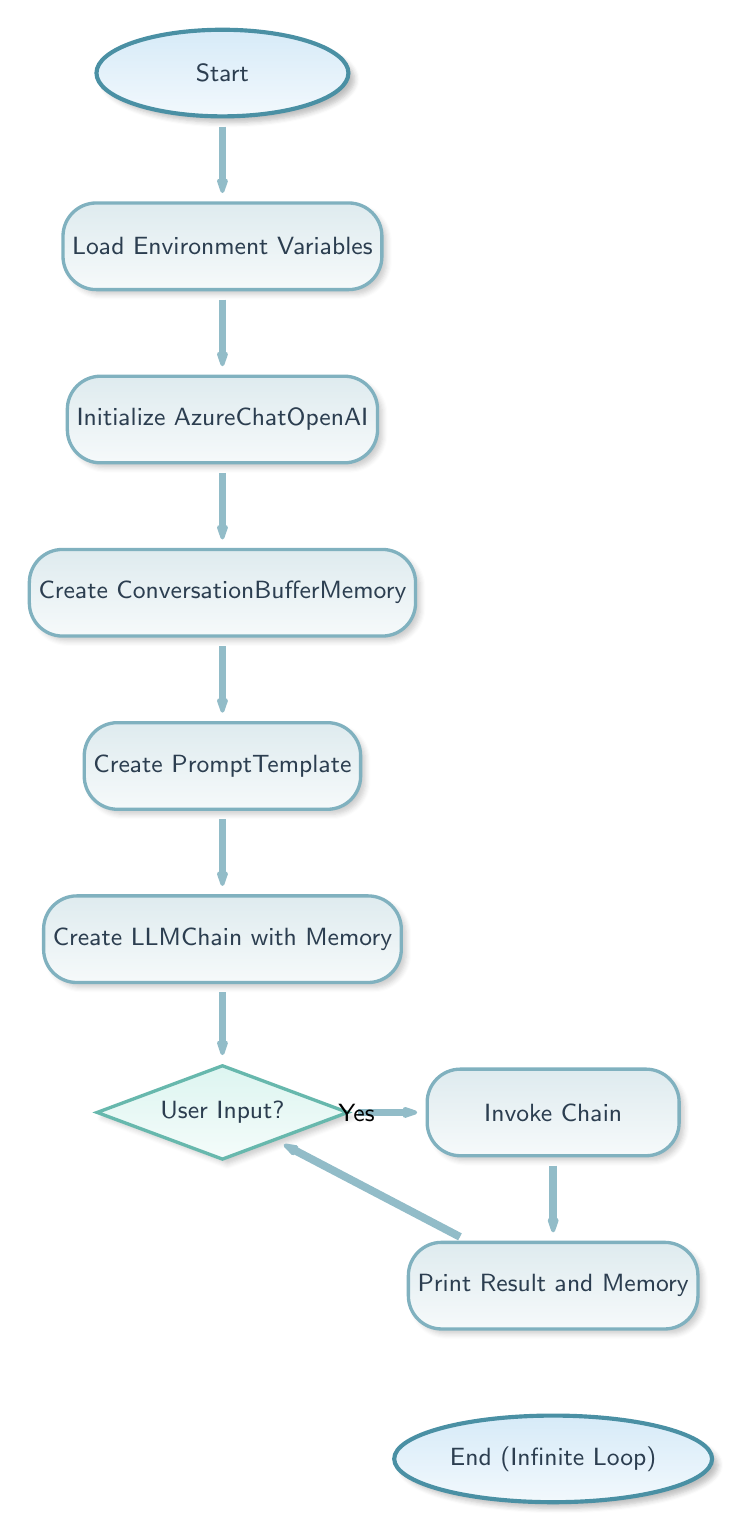
\begin{tikzpicture}[node distance=2.2cm, font=\sffamily\small]
    \node (start) [startstop] {Start};
    \node (load) [process, below of=start] {Load Environment Variables};
    \node (init_llm) [process, below of=load] {Initialize AzureChatOpenAI};
    \node (create_memory) [process, below of=init_llm] {Create ConversationBufferMemory};
    \node (create_prompt) [process, below of=create_memory] {Create PromptTemplate};
    \node (create_chain) [process, below of=create_prompt] {Create LLMChain with Memory};
    \node (loop) [decision, below of=create_chain] {User Input?};
    \node (invoke) [process, right of=loop, xshift=2cm] {Invoke Chain};
    \node (print) [process, below of=invoke] {Print Result and Memory};
    \node (end) [startstop, below of=print] {End (Infinite Loop)};

    \draw [arrow] (start) -- (load);
    \draw [arrow] (load) -- (init_llm);
    \draw [arrow] (init_llm) -- (create_memory);
    \draw [arrow] (create_memory) -- (create_prompt);
    \draw [arrow] (create_prompt) -- (create_chain);
    \draw [arrow] (create_chain) -- (loop);
    \draw [arrow] (loop) -- node[anchor=east] {Yes} (invoke);
    \draw [arrow] (invoke) -- (print);
    \draw [arrow] (print) -- (loop);
\end{tikzpicture}

\section{Ollama Equivalent Code}
\begin{lstlisting}[language=Python]
from langchain_ollama import OllamaLLM
from langchain_core.prompts import PromptTemplate
from langchain_classic.memory import ConversationBufferMemory

llm = OllamaLLM(model="qwen3:4b", temperature=0.7)

memory = ConversationBufferMemory(
    memory_key="chat_history",
    return_messages=True,
)

prompt = PromptTemplate(
    input_variables=["chat_history", "user_input"],
    template="""

   "summary in 50 words technical

    Conversation history:
    {chat_history}
    User: {user_input}
    AI:
    """
)

# Using pipe operator instead of deprecated LLMChain
chain = prompt | llm

while True:
    inp = input("Enter the query: ")
    result = chain.invoke({"user_input": inp, "chat_history": memory.buffer})
    print(result)
    memory.save_context({"input": inp}, {"output": result})
\end{lstlisting}

\subsection{Diff Explanation}
\begin{removedcode}
\begin{diffverb}
- from langchain.chat_models import AzureChatOpenAI
- import os
- from dotenv import load_dotenv
- load_dotenv()
- from langchain.chains import LLMChain
- from langchain.prompts import PromptTemplate
- from langchain.memory import ConversationBufferMemory
- llm_object = AzureChatOpenAI(...)
- chain = LLMChain(llm=llm_object, prompt=prompt, memory=memory)
- result = chain.invoke({"user_input": inp})
- print(result['text'])
- print(memory.buffer)
\end{diffverb}
\end{removedcode}

\begin{addedcode}
\begin{diffverb}
+ from langchain_ollama import OllamaLLM
+ from langchain_core.prompts import PromptTemplate
+ from langchain_classic.memory import ConversationBufferMemory
+ llm = OllamaLLM(model="qwen3:4b", temperature=0.7)
+ chain = prompt | llm
+ result = chain.invoke({"user_input": inp, "chat_history": memory.buffer})
+ print(result)
+ memory.save_context({"input": inp})
\end{diffverb}
\end{addedcode}


\subsection{Explanation of the Diff}
\begin{itemize}
    \item \textbf{Removed Azure setup:} No env vars or cloud API.
    \item \textbf{Updated imports:} Used langchain\_core and langchain\_classic for memory.
    \item \textbf{Changed chaining:} | operator instead of LLMChain.
    \item \textbf{Manual memory update:} Since | chain doesn't auto-update memory, save\_context is called manually.
    \item \textbf{Why:} Adapts conversational memory to Ollama with modern LangChain, requiring explicit memory management.
\end{itemize}

\section{Hugging Face Equivalent Code}
\begin{lstlisting}[language=Python]
from transformers import pipeline

pipe = pipeline("text-generation", model="Qwen/Qwen3-0.6B")

chat_history = []

while True:
    inp = input("Enter the query: ")
    history_str = "\n".join(chat_history)
    prompt = f"""

   "summary in 50 words technical

    Conversation history:
    {history_str}
    User: {inp}
    AI:
    """
    result = pipe(prompt, max_new_tokens=100, temperature=0.7, num_return_sequences=1)
    response = result[0]['generated_text'].split("AI:")[-1].strip() if "AI:" in result[0]['generated_text'] else result[0]['generated_text']
    print(response)
    chat_history.append(f"User: {inp}")
    chat_history.append(f"AI: {response}")
    print(chat_history)
\end{lstlisting}

\subsection{Diff Explanation}
\begin{removedcode}
\begin{diffverb}
- from langchain.chat_models import AzureChatOpenAI
- ... (all LangChain components)
- memory = ConversationBufferMemory(...)
- chain = LLMChain(...)
- result = chain.invoke({"user_input": inp})
- print(result['text'])
- print(memory.buffer)
\end{diffverb}
\end{removedcode}

\begin{addedcode}
\begin{diffverb}
+ from transformers import pipeline
+ pipe = pipeline("text-generation", model="Qwen/Qwen3-0.6B")
+ chat_history = []
+ history_str = "\n".join(chat_history)
+ prompt = f"..." (manual prompt building)
+ result = pipe(prompt, max_new_tokens=100, temperature=0.7, num_return_sequences=1)
+ response = result[0]['generated_text'].split("AI:")[-1].strip() ...
+ print(response)
+ chat_history.append(f"User: {inp}"
+ chat_history.append(f"AI: {response}"
+ print(chat_history)
\end{diffverb}
\end{addedcode}


\subsection{Explanation of the Diff}
\begin{itemize}
    \item \textbf{Removed LangChain memory:} No built-in memory management.
    \item \textbf{Manual history tracking:} Used list to store and build prompt.
    \item \textbf{Prompt engineering:} Constructed prompt string manually with history.
    \item \textbf{Response parsing:} Extracted response from generated text.
    \item \textbf{Why:} Hugging Face requires custom implementation for conversational memory, as it lacks LangChain's abstractions.
\end{itemize}


% ===== CODE9A =====
\newpage
\section{Original Code: code9A.py}
\begin{lstlisting}[language=Python]
from langchain.chat_models import AzureChatOpenAI
import os
from dotenv import load_dotenv
load_dotenv()
from langchain.chains import LLMChain
from langchain.prompts import PromptTemplate
from langchain.memory import ConversationBufferWindowMemory

llm_object = AzureChatOpenAI(
    openai_api_base=os.getenv("AZURE_OPENAI_API_BASE"),
    openai_api_version=os.getenv("AZURE_OPENAI_API_VERSION"),
    openai_api_key=os.getenv("AZURE_OPENAI_API_KEY"),
    deployment_name=os.getenv("AZURE_OPENAI_DEPLOYMENT_NAME"),
    model_name="gpt-4o",
    temperature=0.7,
)

memory = ConversationBufferWindowMemory(
    memory_key="chat_history",
    return_messages=True,
    k=2
)

prompt = PromptTemplate(
    input_variables=["chat_history", "user_input"],
    template="""

   "summary in 50 words technical

    Conversation history:
    {chat_history}
    User: {user_input}
    AI:
    """
)

chain = LLMChain(
    llm=llm_object,
    prompt=prompt,
    memory=memory
)

while True:
    inp = input("Enter the query: ")
    result = chain.invoke({"user_input": inp})
    print(result['text'])
    print(memory.buffer)
\end{lstlisting}

\subsection{Explanation of the Code}
\begin{itemize}
    \item \textbf{What:} This code implements a conversational AI with windowed memory (keeping only the last 2 interactions) using Azure OpenAI and LangChain's ConversationBufferWindowMemory. It loops for user input, generates context-aware responses, and prints the result and memory buffer.
    \item \textbf{Why:} Demonstrates memory management to prevent context from growing indefinitely, focusing on recent history for efficiency. Useful for long conversations where old context becomes less relevant. Uses Azure for consistent AI performance.
    \item \textbf{How:}
    \begin{itemize}
        \item Load env vars.
        \item Init AzureChatOpenAI.
        \item Create ConversationBufferWindowMemory with k=2 (last 2 turns).
        \item Define prompt with history and input.
        \item Create LLMChain with memory.
        \item Loop: Input, invoke, print result['text'] and memory.buffer.
    \end{itemize}
\end{itemize}

\subsection{Flowchart}
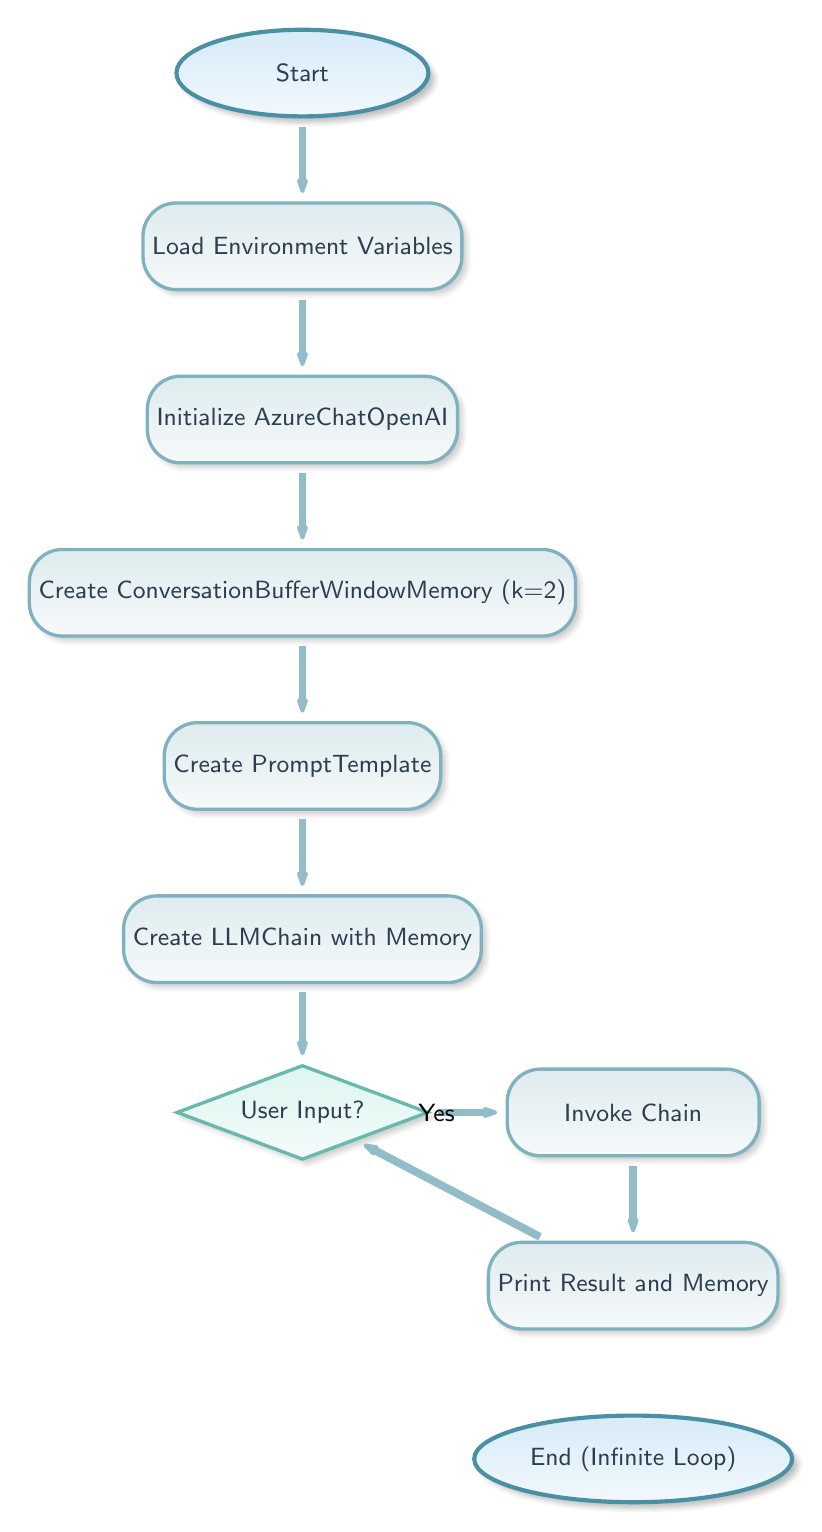
\begin{tikzpicture}[node distance=2.2cm, font=\sffamily\small]
    \node (start) [startstop] {Start};
    \node (load) [process, below of=start] {Load Environment Variables};
    \node (init_llm) [process, below of=load] {Initialize AzureChatOpenAI};
    \node (create_memory) [process, below of=init_llm] {Create ConversationBufferWindowMemory (k=2)};
    \node (create_prompt) [process, below of=create_memory] {Create PromptTemplate};
    \node (create_chain) [process, below of=create_prompt] {Create LLMChain with Memory};
    \node (loop) [decision, below of=create_chain] {User Input?};
    \node (invoke) [process, right of=loop, xshift=2cm] {Invoke Chain};
    \node (print) [process, below of=invoke] {Print Result and Memory};
    \node (end) [startstop, below of=print] {End (Infinite Loop)};

    \draw [arrow] (start) -- (load);
    \draw [arrow] (load) -- (init_llm);
    \draw [arrow] (init_llm) -- (create_memory);
    \draw [arrow] (create_memory) -- (create_prompt);
    \draw [arrow] (create_prompt) -- (create_chain);
    \draw [arrow] (create_chain) -- (loop);
    \draw [arrow] (loop) -- node[anchor=east] {Yes} (invoke);
    \draw [arrow] (invoke) -- (print);
    \draw [arrow] (print) -- (loop);
\end{tikzpicture}

\section{Ollama Equivalent Code}
\begin{lstlisting}[language=Python]
from langchain_ollama import OllamaLLM
from langchain_core.prompts import PromptTemplate
from langchain_classic.memory import ConversationBufferWindowMemory

llm_object = OllamaLLM(model="qwen3:4b", temperature=0.7)

memory = ConversationBufferWindowMemory(
    memory_key="chat_history",
    return_messages=True,
    k=2
)

prompt = PromptTemplate(
    input_variables=["chat_history", "user_input"],
    template="""

   "summary in 50 words technical

    Conversation history:
    {chat_history}
    User: {user_input}
    AI:
    """
)

# Using pipe operator instead of deprecated LLMChain
chain = prompt | llm_object

while True:
    inp = input("Enter the query: ")
    result = chain.invoke({"user_input": inp, "chat_history": memory.buffer})
    print(result)
    memory.save_context({"input": inp}, {"output": result})
\end{lstlisting}

\subsection{Diff Explanation}
\begin{removedcode}
\begin{diffverb}
- from langchain.chat_models import AzureChatOpenAI
- import os
- from dotenv import load_dotenv
- load_dotenv()
- from langchain.chains import LLMChain
- from langchain.prompts import PromptTemplate
- from langchain.memory import ConversationBufferWindowMemory
- llm_object = AzureChatOpenAI(...)
- chain = LLMChain(llm=llm_object, prompt=prompt, memory=memory)
- result = chain.invoke({"user_input": inp})
- print(result['text'])
- print(memory.buffer)
\end{diffverb}
\end{removedcode}

\begin{addedcode}
\begin{diffverb}
+ from langchain_ollama import OllamaLLM
+ from langchain_core.prompts import PromptTemplate
+ from langchain_classic.memory import ConversationBufferWindowMemory
+ llm_object = OllamaLLM(model="qwen3:4b", temperature=0.7)
+ chain = prompt | llm_object
+ result = chain.invoke({"user_input": inp, "chat_history": memory.buffer})
+ print(result)
+ memory.save_context({"input": inp})
\end{diffverb}
\end{addedcode}


\subsection{Explanation of the Diff}
\begin{itemize}
    \item \textbf{Removed Azure setup:} Local Ollama instead.
    \item \textbf{Updated imports:} langchain\_core and langchain\_classic.
    \item \textbf{Modern chaining:} | operator.
    \item \textbf{Manual memory save:} Required for | chains.
    \item \textbf{Why:} Adapts windowed memory to Ollama with updated LangChain patterns.
\end{itemize}

\section{Hugging Face Equivalent Code}
\begin{lstlisting}[language=Python]
from transformers import pipeline

pipe = pipeline("text-generation", model="Qwen/Qwen3-0.6B")

chat_history = []

while True:
    inp = input("Enter the query: ")
    # Keep only last 2 exchanges (4 messages: 2 user + 2 AI)
    if len(chat_history) > 4:
        chat_history = chat_history[-4:]
    history_str = "\n".join(chat_history)
    prompt = f"""

   "summary in 50 words technical

    Conversation history:
    {history_str}
    User: {inp}
    AI:
    """
    result = pipe(prompt, max_new_tokens=100, temperature=0.7, num_return_sequences=1)
    response = result[0]['generated_text'].split("AI:")[-1].strip() if "AI:" in result[0]['generated_text'] else result[0]['generated_text']
    print(response)
    chat_history.append(f"User: {inp}")
    chat_history.append(f"AI: {response}")
    print(chat_history)
\end{lstlisting}

\subsection{Diff Explanation}
\begin{removedcode}
\begin{diffverb}
- from langchain.chat_models import AzureChatOpenAI
- ... (all LangChain)
- memory = ConversationBufferWindowMemory(...)
- chain = LLMChain(...)
- result = chain.invoke({"user_input": inp})
- print(result['text'])
- print(memory.buffer)
\end{diffverb}
\end{removedcode}

\begin{addedcode}
\begin{diffverb}
+ from transformers import pipeline
+ pipe = pipeline("text-generation", model="Qwen/Qwen3-0.6B")
+ chat_history = []
+ if len(chat_history) > 4: chat_history = chat_history[-4:]
+ history_str = "\n".join(chat_history)
+ prompt = f"..." (manual)
+ result = pipe(prompt, max_new_tokens=100, temperature=0.7, num_return_sequences=1)
+ response = result[0]['generated_text'].split("AI:")[-1].strip() ...
+ print(response)
+ chat_history.append(f"User: {inp}"
+ chat_history.append(f"AI: {response}"
+ print(chat_history)
\end{diffverb}
\end{addedcode}


\subsection{Explanation of the Diff}
\begin{itemize}
    \item \textbf{Removed LangChain memory:} Custom window implementation.
    \item \textbf{Manual windowing:} Truncate history to last 4 messages.
    \item \textbf{Prompt building:} String concatenation for history.
    \item \textbf{Why:} Hugging Face requires manual memory and prompt management for windowed conversations.
\end{itemize}


% ===== CODE9B =====
\newpage
\section{Original Code: code9B.py}
\begin{lstlisting}[language=Python]
from langchain.chat_models import AzureChatOpenAI
import os
from dotenv import load_dotenv
load_dotenv()
from langchain.chains import LLMChain
from langchain.prompts import PromptTemplate
from langchain.memory import ConversationSummaryMemory

llm_object = AzureChatOpenAI(
    openai_api_base=os.getenv("AZURE_OPENAI_API_BASE"),
    openai_api_version=os.getenv("AZURE_OPENAI_API_VERSION"),
    openai_api_key=os.getenv("AZURE_OPENAI_API_KEY"),
    deployment_name=os.getenv("AZURE_OPENAI_DEPLOYMENT_NAME"),
    model_name="gpt-4o",
    temperature=0.7,
)

memory = ConversationSummaryMemory(
    memory_key="chat_history",
    return_messages=True,
    llm=llm
)

prompt = PromptTemplate(
    input_variables=["chat_history", "user_input"],
    template="""

   "summary in 50 words technical

    Conversation history:
    {chat_history}
    User: {user_input}
    AI:
    """
)

chain = LLMChain(
    llm=llm_object,
    prompt=prompt,
    memory=memory
)

while True:
    inp = input("Enter the query: ")
    result = chain.invoke({"user_input": inp})
    print(result['text'])
    print(memory.buffer)
\end{lstlisting}

\subsection{Explanation of the Code}
\begin{itemize}
    \item \textbf{What:} This code uses ConversationSummaryMemory to maintain a summarized version of the conversation history, condensing past interactions into summaries. It employs Azure OpenAI in a loop for user queries, printing responses and the current memory summary.
    \item \textbf{Why:} Summary memory prevents context from growing too large by summarizing old parts, maintaining efficiency in long conversations. Useful when full history isn't needed but key points are. Leverages Azure for summarization and response generation.
    \item \textbf{How:}
    \begin{itemize}
        \item Load env vars.
        \item Init AzureChatOpenAI (note: llm in memory should be llm\_object).
        \item Create ConversationSummaryMemory with llm for summarization.
        \item Define prompt with history and input.
        \item Create LLMChain with memory.
        \item Loop: Input, invoke, print result['text'] and memory.buffer (summary).
    \end{itemize}
\end{itemize}

\subsection{Flowchart}
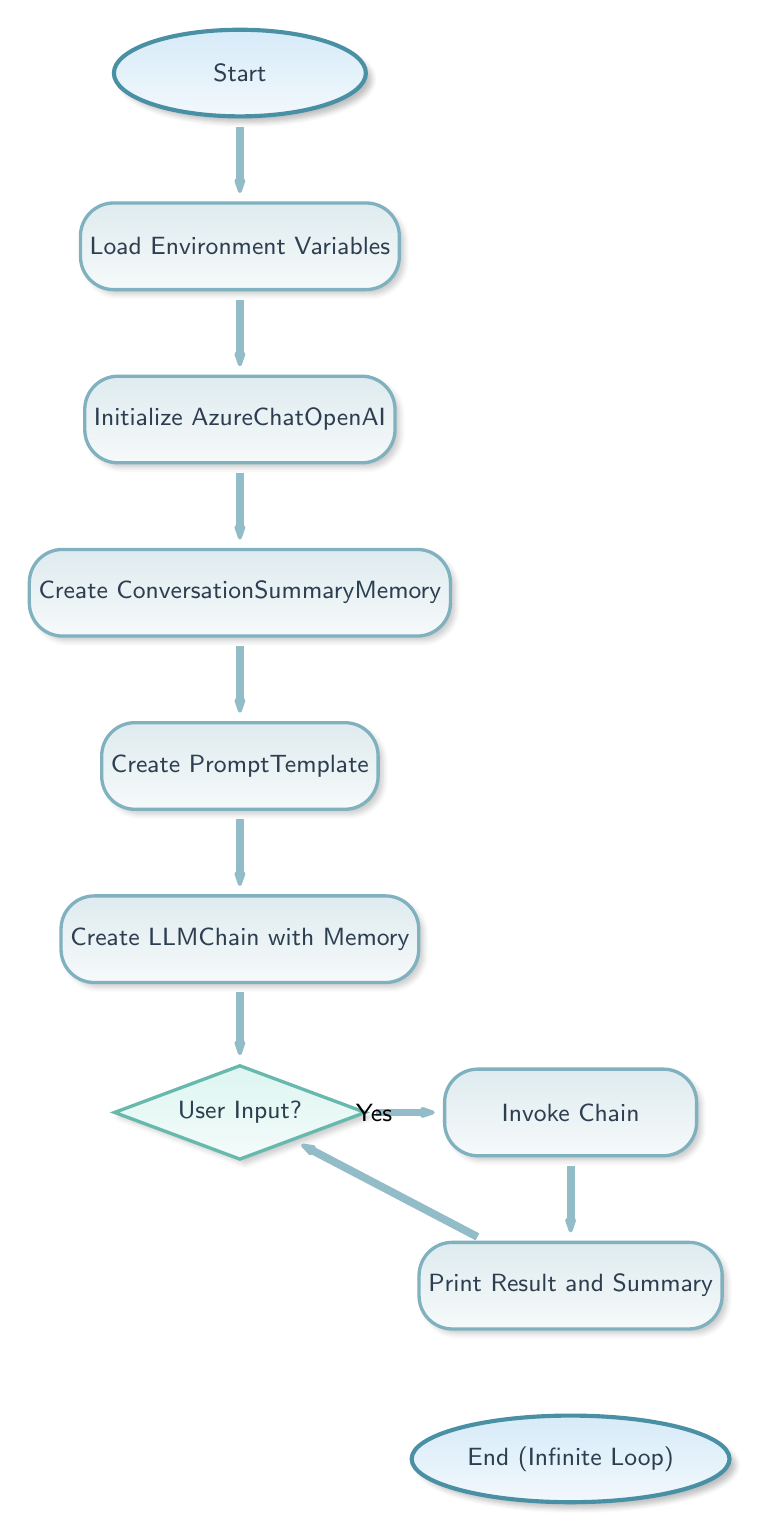
\begin{tikzpicture}[node distance=2.2cm, font=\sffamily\small]
    \node (start) [startstop] {Start};
    \node (load) [process, below of=start] {Load Environment Variables};
    \node (init_llm) [process, below of=load] {Initialize AzureChatOpenAI};
    \node (create_memory) [process, below of=init_llm] {Create ConversationSummaryMemory};
    \node (create_prompt) [process, below of=create_memory] {Create PromptTemplate};
    \node (create_chain) [process, below of=create_prompt] {Create LLMChain with Memory};
    \node (loop) [decision, below of=create_chain] {User Input?};
    \node (invoke) [process, right of=loop, xshift=2cm] {Invoke Chain};
    \node (print) [process, below of=invoke] {Print Result and Summary};
    \node (end) [startstop, below of=print] {End (Infinite Loop)};

    \draw [arrow] (start) -- (load);
    \draw [arrow] (load) -- (init_llm);
    \draw [arrow] (init_llm) -- (create_memory);
    \draw [arrow] (create_memory) -- (create_prompt);
    \draw [arrow] (create_prompt) -- (create_chain);
    \draw [arrow] (create_chain) -- (loop);
    \draw [arrow] (loop) -- node[anchor=east] {Yes} (invoke);
    \draw [arrow] (invoke) -- (print);
    \draw [arrow] (print) -- (loop);
\end{tikzpicture}

\section{Ollama Equivalent Code}
\begin{lstlisting}[language=Python]
from langchain_ollama import OllamaLLM
from langchain_core.prompts import PromptTemplate
from langchain_classic.memory import ConversationSummaryMemory

llm_object = OllamaLLM(model="qwen3:4b", temperature=0.7)

memory = ConversationSummaryMemory(
    memory_key="chat_history",
    return_messages=True,
    llm=llm_object
)

prompt = PromptTemplate(
    input_variables=["chat_history", "user_input"],
    template="""

   "summary in 50 words technical

    Conversation history:
    {chat_history}
    User: {user_input}
    AI:
    """
)

# Using pipe operator instead of deprecated LLMChain
chain = prompt | llm_object

while True:
    inp = input("Enter the query: ")
    result = chain.invoke({"user_input": inp, "chat_history": memory.buffer})
    print(result)
    memory.save_context({"input": inp}, {"output": result})
\end{lstlisting}

\subsection{Diff Explanation}
\begin{removedcode}
\begin{diffverb}
- from langchain.chat_models import AzureChatOpenAI
- import os
- from dotenv import load_dotenv
- load_dotenv()
- from langchain.chains import LLMChain
- from langchain.prompts import PromptTemplate
- from langchain.memory import ConversationSummaryMemory
- llm_object = AzureChatOpenAI(...)
- memory = ConversationSummaryMemory(..., llm=llm)
- chain = LLMChain(llm=llm_object, prompt=prompt, memory=memory)
- result = chain.invoke({"user_input": inp})
- print(result['text'])
- print(memory.buffer)
\end{diffverb}
\end{removedcode}

\begin{addedcode}
\begin{diffverb}
+ from langchain_ollama import OllamaLLM
+ from langchain_core.prompts import PromptTemplate
+ from langchain_classic.memory import ConversationSummaryMemory
+ llm_object = OllamaLLM(model="qwen3:4b", temperature=0.7)
+ memory = ConversationSummaryMemory(..., llm=llm_object)
+ chain = prompt | llm_object
+ result = chain.invoke({"user_input": inp, "chat_history": memory.buffer})
+ print(result)
+ memory.save_context({"input": inp})
\end{diffverb}
\end{addedcode}


\subsection{Explanation of the Diff}
\begin{itemize}
    \item \textbf{Removed Azure:} Local Ollama.
    \item \textbf{Updated imports:} langchain\_core and langchain\_classic.
    \item \textbf{Modern chaining:} | operator.
    \item \textbf{Manual save:} For memory update.
    \item \textbf{Why:} Adapts summary memory to Ollama, using the same LLM for summarization.
\end{itemize}

\section{Hugging Face Equivalent Code}
\begin{lstlisting}[language=Python]
from transformers import pipeline

pipe = pipeline("text-generation", model="Qwen/Qwen3-0.6B")

chat_history = []

while True:
    inp = input("Enter the query: ")
    history_str = "\n".join(chat_history)
    prompt = f"""

   "summary in 50 words technical

    Conversation history:
    {history_str}
    User: {inp}
    AI:
    """
    result = pipe(prompt, max_new_tokens=100, temperature=0.7, num_return_sequences=1)
    response = result[0]['generated_text'].split("AI:")[-1].strip() if "AI:" in result[0]['generated_text'] else result[0]['generated_text']
    print(response)
    chat_history.append(f"User: {inp}")
    chat_history.append(f"AI: {response}")
    print(chat_history)
\end{lstlisting}

\subsection{Diff Explanation}
\begin{removedcode}
\begin{diffverb}
- from langchain.chat_models import AzureChatOpenAI
- ... (all LangChain)
- memory = ConversationSummaryMemory(...)
- chain = LLMChain(...)
- result = chain.invoke({"user_input": inp})
- print(result['text'])
- print(memory.buffer)
\end{diffverb}
\end{removedcode}

\begin{addedcode}
\begin{diffverb}
+ from transformers import pipeline
+ pipe = pipeline("text-generation", model="Qwen/Qwen3-0.6B")
+ chat_history = []
+ history_str = "\n".join(chat_history)
+ prompt = f"..." (manual)
+ result = pipe(prompt, max_new_tokens=100, temperature=0.7, num_return_sequences=1)
+ response = result[0]['generated_text'].split("AI:")[-1].strip() ...
+ print(response)
+ chat_history.append(f"User: {inp}"
+ chat_history.append(f"AI: {response}"
+ print(chat_history)
\end{diffverb}
\end{addedcode}


\subsection{Explanation of the Diff}
\begin{itemize}
    \item \textbf{Removed summary memory:} No summarization, full history.
    \item \textbf{Manual history:} List-based tracking.
    \item \textbf{Why:} Hugging Face lacks built-in summary memory, so simplified to buffer-like behavior.
\end{itemize}


% ===== CODE9C =====
\newpage
\section{Original Code: code9C.py}
\begin{lstlisting}[language=Python]
from langchain.chat_models import AzureChatOpenAI
import os
from dotenv import load_dotenv
load_dotenv()
from langchain.chains import LLMChain
from langchain.prompts import PromptTemplate
from langchain.memory import ConversationSummaryWindowMemory

llm_object = AzureChatOpenAI(
    openai_api_base=os.getenv("AZURE_OPENAI_API_BASE"),
    openai_api_version=os.getenv("AZURE_OPENAI_API_VERSION"),
    openai_api_key=os.getenv("AZURE_OPENAI_API_KEY"),
    deployment_name=os.getenv("AZURE_OPENAI_DEPLOYMENT_NAME"),
    model_name="gpt-4o",
    temperature=0.7,
)

memory = ConversationSummaryWindowMemory(
    memory_key="chat_history",
    return_messages=True,
    llm=llm,
    k=2
)

prompt = PromptTemplate(
    input_variables=["chat_history", "user_input"],
    template="""

   "summary in 50 words technical

    Conversation history:
    {chat_history}
    User: {user_input}
    AI:
    """
)

chain = LLMChain(
    llm=llm_object,
    prompt=prompt,
    memory=memory
)

while True:
    inp = input("Enter the query: ")
    result = chain.invoke({"user_input": inp})
    print(result['text'])
    print(memory.buffer)
\end{lstlisting}

\subsection{Explanation of the Code}
\begin{itemize}
    \item \textbf{What:} This code employs ConversationSummaryWindowMemory, which summarizes the conversation but keeps the last k interactions in full. It uses Azure OpenAI in a loop, printing responses and the summarized/windowed memory.
    \item \textbf{Why:} Combines summarization for old parts with full retention of recent interactions, balancing efficiency and recency. Ideal for conversations needing recent context but compressed history. Uses Azure for both generation and summarization.
    \item \textbf{How:}
    \begin{itemize}
        \item Load env vars.
        \item Init AzureChatOpenAI.
        \item Create ConversationSummaryWindowMemory with llm (should be llm\_object) and k=2.
        \item Define prompt.
        \item Create LLMChain.
        \item Loop: Input, invoke, print result['text'] and memory.buffer.
    \end{itemize}
\end{itemize}

\subsection{Flowchart}
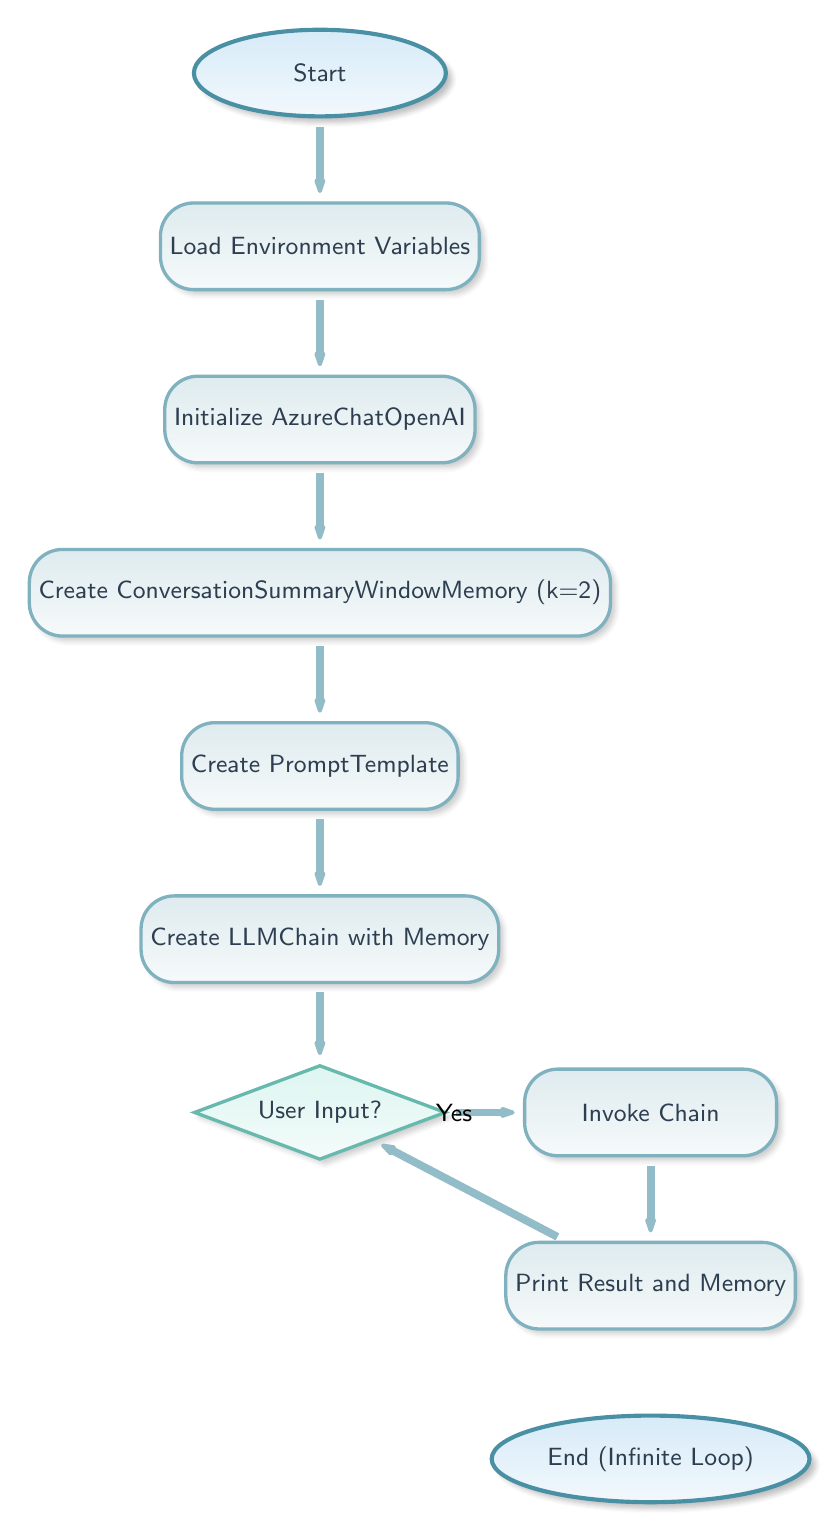
\begin{tikzpicture}[node distance=2.2cm, font=\sffamily\small]
    \node (start) [startstop] {Start};
    \node (load) [process, below of=start] {Load Environment Variables};
    \node (init_llm) [process, below of=load] {Initialize AzureChatOpenAI};
    \node (create_memory) [process, below of=init_llm] {Create ConversationSummaryWindowMemory (k=2)};
    \node (create_prompt) [process, below of=create_memory] {Create PromptTemplate};
    \node (create_chain) [process, below of=create_prompt] {Create LLMChain with Memory};
    \node (loop) [decision, below of=create_chain] {User Input?};
    \node (invoke) [process, right of=loop, xshift=2cm] {Invoke Chain};
    \node (print) [process, below of=invoke] {Print Result and Memory};
    \node (end) [startstop, below of=print] {End (Infinite Loop)};

    \draw [arrow] (start) -- (load);
    \draw [arrow] (load) -- (init_llm);
    \draw [arrow] (init_llm) -- (create_memory);
    \draw [arrow] (create_memory) -- (create_prompt);
    \draw [arrow] (create_prompt) -- (create_chain);
    \draw [arrow] (create_chain) -- (loop);
    \draw [arrow] (loop) -- node[anchor=east] {Yes} (invoke);
    \draw [arrow] (invoke) -- (print);
    \draw [arrow] (print) -- (loop);
\end{tikzpicture}

\section{Ollama Equivalent Code}
\begin{lstlisting}[language=Python]
from langchain_ollama import OllamaLLM
from langchain_core.prompts import PromptTemplate
from langchain_classic.memory import ConversationSummaryBufferMemory

llm_object = OllamaLLM(model="qwen3:4b", temperature=0.7)

memory = ConversationSummaryBufferMemory(
    memory_key="chat_history",
    return_messages=True,
    llm=llm_object,
)

prompt = PromptTemplate(
    input_variables=["chat_history", "user_input"],
    template="""

   "summary in 50 words technical

    Conversation history:
    {chat_history}
    User: {user_input}
    AI:
    """
)

# Using pipe operator instead of deprecated LLMChain
chain = prompt | llm_object

while True:
    inp = input("Enter the query: ")
    result = chain.invoke({"user_input": inp, "chat_history": memory.buffer})
    print(result)
    memory.save_context({"input": inp}, {"output": result})
\end{lstlisting}

\subsection{Diff Explanation}
\begin{removedcode}
\begin{diffverb}
- from langchain.chat_models import AzureChatOpenAI
- import os
- from dotenv import load_dotenv
- load_dotenv()
- from langchain.chains import LLMChain
- from langchain.prompts import PromptTemplate
- from langchain.memory import ConversationSummaryWindowMemory
- llm_object = AzureChatOpenAI(...)
- memory = ConversationSummaryWindowMemory(..., llm=llm, k=2)
- chain = LLMChain(llm=llm_object, prompt=prompt, memory=memory)
- result = chain.invoke({"user_input": inp})
- print(result['text'])
- print(memory.buffer)
\end{diffverb}
\end{removedcode}

\begin{addedcode}
\begin{diffverb}
+ from langchain_ollama import OllamaLLM
+ from langchain_core.prompts import PromptTemplate
+ from langchain_classic.memory import ConversationSummaryBufferMemory
+ llm_object = OllamaLLM(model="qwen3:4b", temperature=0.7)
+ memory = ConversationSummaryBufferMemory(..., llm=llm_object)
+ chain = prompt | llm_object
+ result = chain.invoke({"user_input": inp, "chat_history": memory.buffer})
+ print(result)
+ memory.save_context({"input": inp})
\end{diffverb}
\end{addedcode}


\subsection{Explanation of the Diff}
\begin{itemize}
    \item \textbf{Removed Azure:} Local Ollama.
    \item \textbf{Changed memory type:} ConversationSummaryBufferMemory instead of Window, as Window may not be available.
    \item \textbf{Modern chaining:} | operator.
    \item \textbf{Why:} Adapts to available memory types in langchain\_classic, using buffer with summarization.
\end{itemize}

\section{Hugging Face Equivalent Code}
\begin{lstlisting}[language=Python]
from transformers import pipeline

pipe = pipeline("text-generation", model="Qwen/Qwen3-0.6B")

chat_history = []

while True:
    inp = input("Enter the query: ")
    # Approximate: keep last 4 messages
    if len(chat_history) > 4:
        chat_history = chat_history[-4:]
    history_str = "\n".join(chat_history)
    prompt = f"""

   "summary in 50 words technical

    Conversation history:
    {history_str}
    User: {inp}
    AI:
    """
    result = pipe(prompt, max_new_tokens=100, temperature=0.7, num_return_sequences=1)
    response = result[0]['generated_text'].split("AI:")[-1].strip() if "AI:" in result[0]['generated_text'] else result[0]['generated_text']
    print(response)
    chat_history.append(f"User: {inp}")
    chat_history.append(f"AI: {response}")
    print(chat_history)
\end{lstlisting}

\subsection{Diff Explanation}
\begin{removedcode}
\begin{diffverb}
- from langchain.chat_models import AzureChatOpenAI
- ... (all LangChain)
- memory = ConversationSummaryWindowMemory(...)
- chain = LLMChain(...)
- result = chain.invoke({"user_input": inp})
- print(result['text'])
- print(memory.buffer)
\end{diffverb}
\end{removedcode}

\begin{addedcode}
\begin{diffverb}
+ from transformers import pipeline
+ pipe = pipeline("text-generation", model="Qwen/Qwen3-0.6B")
+ chat_history = []
+ if len(chat_history) > 4: chat_history = chat_history[-4:]
+ history_str = "\n".join(chat_history)
+ prompt = f"..." (manual)
+ result = pipe(prompt, max_new_tokens=100, temperature=0.7, num_return_sequences=1)
+ response = result[0]['generated_text'].split("AI:")[-1].strip() ...
+ print(response)
+ chat_history.append(f"User: {inp}"
+ chat_history.append(f"AI: {response}"
+ print(chat_history)
\end{diffverb}
\end{addedcode}


\subsection{Explanation of the Diff}
\begin{itemize}
    \item \textbf{Removed summary window memory:} Manual windowing without summarization.
    \item \textbf{Why:} Hugging Face doesn't have built-in summary memory, so approximated with buffer window.
\end{itemize}


% ===== CODE10 =====
\newpage
\section{Original Code: code10.py}
\begin{lstlisting}[language=Python]
#component 1 LLM
from langchain.chat_models import AzureChatOpenAI
import os
from dotenv import load_dotenv
load_dotenv()
llm = AzureChatOpenAI(
    openai_api_base=os.getenv("AZURE_OPENAI_API_BASE"),
    openai_api_version=os.getenv("AZURE_OPENAI_API_VERSION"),
    openai_api_key=os.getenv("AZURE_OPENAI_API_KEY"),
    deployment_name=os.getenv("AZURE_OPENAI_DEPLOYMENT_NAME"),
    model_name="gpt-4o",
    temperature=0.7,
)


from langchain.chains import LLMChain

#compenent 2 PROMPT
from langchain.prompts import PromptTemplate
prompt=PromptTemplate(
    template="what is the capital of {input}"
)

pipeline=LLMChain(
    llm=llm,
    prompt=prompt
)


result=pipeline.invoke(input="china")

print(result['text'])
\end{lstlisting}

\subsection{Explanation of the Code}
\begin{itemize}
    \item \textbf{What:} This code creates a simple pipeline using LLMChain that combines a prompt template with Azure OpenAI LLM, invokes it with "china" as input, and prints the response.
    \item \textbf{Why:} Demonstrates basic chaining of prompt and LLM in LangChain for templated queries. Uses Azure for cloud-based AI, with env vars for security.
    \item \textbf{How:}
    \begin{itemize}
        \item Load env vars.
        \item Init AzureChatOpenAI.
        \item Create PromptTemplate with placeholder.
        \item Create LLMChain with llm and prompt.
        \item Invoke with dict input.
        \item Print result['text'].
    \end{itemize}
\end{itemize}

\subsection{Flowchart}
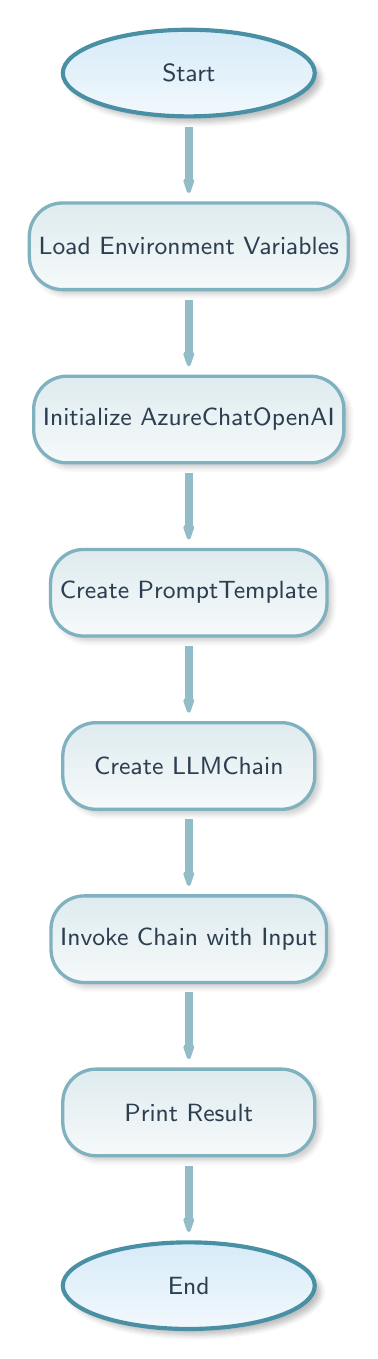
\begin{tikzpicture}[node distance=2.2cm, font=\sffamily\small]
    \node (start) [startstop] {Start};
    \node (load) [process, below of=start] {Load Environment Variables};
    \node (init_llm) [process, below of=load] {Initialize AzureChatOpenAI};
    \node (create_prompt) [process, below of=init_llm] {Create PromptTemplate};
    \node (create_chain) [process, below of=create_prompt] {Create LLMChain};
    \node (invoke) [process, below of=create_chain] {Invoke Chain with Input};
    \node (print) [process, below of=invoke] {Print Result};
    \node (end) [startstop, below of=print] {End};

    \draw [arrow] (start) -- (load);
    \draw [arrow] (load) -- (init_llm);
    \draw [arrow] (init_llm) -- (create_prompt);
    \draw [arrow] (create_prompt) -- (create_chain);
    \draw [arrow] (create_chain) -- (invoke);
    \draw [arrow] (invoke) -- (print);
    \draw [arrow] (print) -- (end);
\end{tikzpicture}

\section{Ollama Equivalent Code}
\begin{lstlisting}[language=Python]
from langchain_ollama import OllamaLLM
from langchain_core.prompts import PromptTemplate

llm = OllamaLLM(model="qwen3:4b", temperature=0.7)

prompt = PromptTemplate(
    template="what is the capital of {input}"
)

# Using pipe operator instead of deprecated LLMChain
pipeline = prompt | llm

result = pipeline.invoke({"input": "china"})

print(result)
\end{lstlisting}

\subsection{Diff Explanation}
\begin{removedcode}
\begin{diffverb}
- from langchain.chat_models import AzureChatOpenAI
- import os
- from dotenv import load_dotenv
- load_dotenv()
- llm = AzureChatOpenAI(...)
- from langchain.chains import LLMChain
- from langchain.prompts import PromptTemplate
- prompt=PromptTemplate(...)
- pipeline=LLMChain(llm=llm, prompt=prompt)
- result=pipeline.invoke(input="china")
- print(result['text'])
\end{diffverb}
\end{removedcode}

\begin{addedcode}
\begin{diffverb}
+ from langchain_ollama import OllamaLLM
+ from langchain_core.prompts import PromptTemplate
+ llm = OllamaLLM(model="qwen3:4b", temperature=0.7)
+ prompt = PromptTemplate(...)
+ pipeline = prompt | llm
+ result = pipeline.invoke({"input": "china"})
+ print(result)
\end{diffverb}
\end{addedcode}


\subsection{Explanation of the Diff}
\begin{itemize}
    \item \textbf{Removed Azure setup:} Local Ollama.
    \item \textbf{Updated imports:} langchain\_core.
    \item \textbf{Modern chaining:} | instead of LLMChain.
    \item \textbf{Why:} Simplifies to local execution with updated LangChain syntax.
\end{itemize}

\section{Hugging Face Equivalent Code}
\begin{lstlisting}[language=Python]
from transformers import pipeline

pipe = pipeline("text-generation", model="Qwen/Qwen3-0.6B")

prompt_template = "what is the capital of {input}"

input_value = "china"
prompt = prompt_template.format(input=input_value)

result = pipe(prompt, max_new_tokens=50, temperature=0.7, num_return_sequences=1)

print(result[0]['generated_text'])
\end{lstlisting}

\subsection{Diff Explanation}
\begin{removedcode}
\begin{diffverb}
- from langchain.chat_models import AzureChatOpenAI
- ... (all LangChain)
- pipeline=LLMChain(...)
- result=pipeline.invoke(input="china")
- print(result['text'])
\end{diffverb}
\end{removedcode}

\begin{addedcode}
\begin{diffverb}
+ from transformers import pipeline
+ pipe = pipeline("text-generation", model="Qwen/Qwen3-0.6B")
+ prompt_template = "what is the capital of {input}"
+ input_value = "china"
+ prompt = prompt_template.format(input=input_value)
+ result = pipe(prompt, max_new_tokens=50, temperature=0.7, num_return_sequences=1)
+ print(result[0]['generated_text'])
\end{diffverb}
\end{addedcode}


\subsection{Explanation of the Diff}
\begin{itemize}
    \item \textbf{Removed LangChain:} Manual template formatting.
    \item \textbf{Direct pipeline:} No chaining abstraction.
    \item \textbf{Why:} Hugging Face requires explicit prompt construction.
\end{itemize}


% ===== CODE11 =====
\newpage
\section{Original Code: code11.py}
\begin{lstlisting}[language=Python]
# Component -1
from langchain.chat_models import AzureChatOpenAI
import os
from dotenv import load_dotenv
load_dotenv()
import streamlit as st
st.title("MY FIRST CHATBOT")
my_llm = AzureChatOpenAI(
    openai_api_base=os.getenv("AZURE_OPENAI_API_BASE"),
    openai_api_version=os.getenv("AZURE_OPENAI_API_VERSION"),
    openai_api_key=os.getenv("AZURE_OPENAI_API_KEY"),
    deployment_name=os.getenv("AZURE_OPENAI_DEPLOYMENT_NAME"),
    model_name="gpt-4o",
    temperature=0.7,
)

# Component -2  (ChatPromptTemplate Version)
from langchain.prompts import ChatPromptTemplate

my_prompt = ChatPromptTemplate.from_messages([
    ("system", "You are a helpful assistant."),
    ("human", "{input}")
])

from langchain.chains import LLMChain

my_pipeline = LLMChain(
    llm=my_llm,
    prompt=my_prompt
)
usertext=st.text_input("USER:")
result = my_pipeline.invoke({"input": usertext})
st.write(result["text"])
\end{lstlisting}

\subsection{Explanation of the Code}
\begin{itemize}
    \item \textbf{What:} This code builds a Streamlit web app for a chatbot, using ChatPromptTemplate with system and human messages, combined with Azure OpenAI in an LLMChain, taking user input and displaying the AI response.
    \item \textbf{Why:} Demonstrates creating a simple web-based chatbot with LangChain's chat prompt templates for structured conversations. Uses Streamlit for UI and Azure for AI.
    \item \textbf{How:}
    \begin{itemize}
        \item Load env vars.
        \item Init Streamlit title.
        \item Init AzureChatOpenAI.
        \item Create ChatPromptTemplate with messages.
        \item Create LLMChain.
        \item Get user input via st.text\_input.
        \item Invoke chain and display result["text"].
    \end{itemize}
\end{itemize}

\subsection{Flowchart}
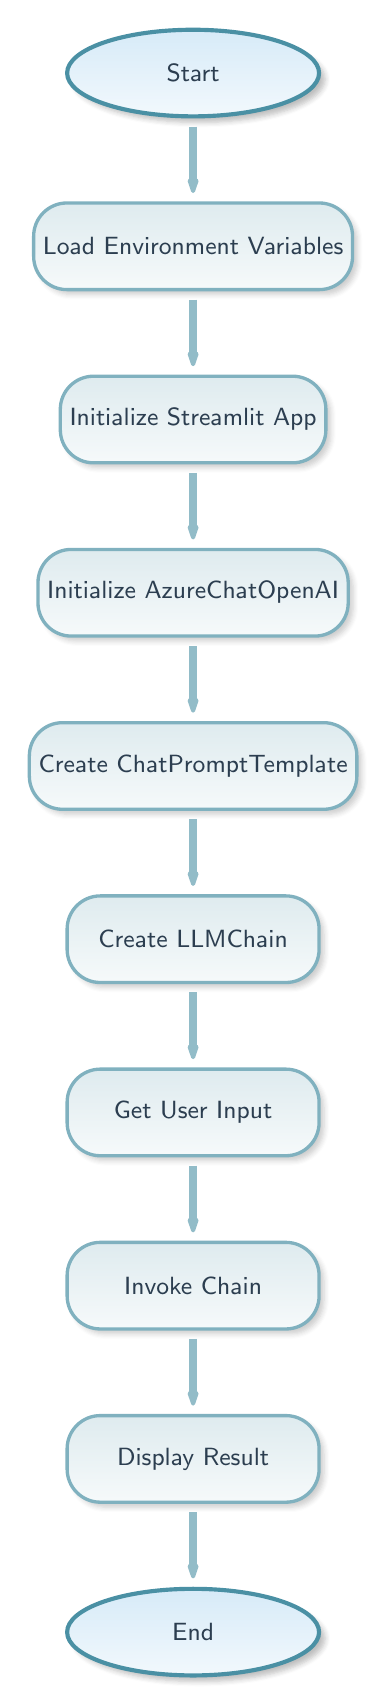
\begin{tikzpicture}[node distance=2.2cm, font=\sffamily\small]
    \node (start) [startstop] {Start};
    \node (load) [process, below of=start] {Load Environment Variables};
    \node (init_st) [process, below of=load] {Initialize Streamlit App};
    \node (init_llm) [process, below of=init_st] {Initialize AzureChatOpenAI};
    \node (create_prompt) [process, below of=init_llm] {Create ChatPromptTemplate};
    \node (create_chain) [process, below of=create_prompt] {Create LLMChain};
    \node (get_input) [process, below of=create_chain] {Get User Input};
    \node (invoke) [process, below of=get_input] {Invoke Chain};
    \node (display) [process, below of=invoke] {Display Result};
    \node (end) [startstop, below of=display] {End};

    \draw [arrow] (start) -- (load);
    \draw [arrow] (load) -- (init_st);
    \draw [arrow] (init_st) -- (init_llm);
    \draw [arrow] (init_llm) -- (create_prompt);
    \draw [arrow] (create_prompt) -- (create_chain);
    \draw [arrow] (create_chain) -- (get_input);
    \draw [arrow] (get_input) -- (invoke);
    \draw [arrow] (invoke) -- (display);
    \draw [arrow] (display) -- (end);
\end{tikzpicture}

\section{Ollama Equivalent Code}
\begin{lstlisting}[language=Python]
# Component -1
from langchain_ollama import OllamaLLM
import streamlit as st
st.title("MY FIRST CHATBOT")
my_llm = OllamaLLM(model="qwen3:4b", temperature=0.7)

# Component -2  (ChatPromptTemplate Version)
from langchain_core.prompts import ChatPromptTemplate

my_prompt = ChatPromptTemplate.from_messages([
    ("system", "You are a helpful assistant."),
    ("human", "{input}")
])

# Using pipe operator instead of deprecated LLMChain
my_pipeline = my_prompt | my_llm
usertext=st.text_input("USER:")
result = my_pipeline.invoke({"input": usertext})
st.write(result["text"])
\end{lstlisting}

\subsection{Diff Explanation}
\begin{removedcode}
\begin{diffverb}
- from langchain.chat_models import AzureChatOpenAI
- import os
- from dotenv import load_dotenv
- load_dotenv()
- my_llm = AzureChatOpenAI(...)
- from langchain.prompts import ChatPromptTemplate
- from langchain.chains import LLMChain
- my_pipeline = LLMChain(llm=my_llm, prompt=my_prompt)
\end{diffverb}
\end{removedcode}

\begin{addedcode}
\begin{diffverb}
+ from langchain_ollama import OllamaLLM
+ my_llm = OllamaLLM(model="qwen3:4b", temperature=0.7)
+ from langchain_core.prompts import ChatPromptTemplate
+ my_pipeline = my_prompt | my_llm
\end{diffverb}
\end{addedcode}


\subsection{Explanation of the Diff}
\begin{itemize}
    \item \textbf{Removed Azure:} Local Ollama.
    \item \textbf{Updated imports:} langchain\_core.
    \item \textbf{Modern chaining:} | operator.
    \item \textbf{Why:} Adapts to local model with updated syntax.
\end{itemize}

\section{Hugging Face Equivalent Code}
\begin{lstlisting}[language=Python]
from transformers import pipeline
import streamlit as st
st.title("MY FIRST CHATBOT")

generator = pipeline("text-generation", model="gpt2")

usertext = st.text_input("USER:")
if usertext:
    prompt = f"You are a helpful assistant. {usertext}"
    result = generator(prompt, max_length=50, num_return_sequences=1)
    st.write(result[0]['generated_text'])
\end{lstlisting}

\subsection{Diff Explanation}
\begin{removedcode}
\begin{diffverb}
- from langchain.chat_models import AzureChatOpenAI
- ... (all LangChain)
- my_pipeline = LLMChain(...)
- result = my_pipeline.invoke({"input": usertext})
- st.write(result["text"])
\end{diffverb}
\end{removedcode}

\begin{addedcode}
\begin{diffverb}
+ from transformers import pipeline
+ generator = pipeline("text-generation", model="gpt2")
+ usertext = st.text_input("USER:")
+ if usertext:
+     prompt = f"You are a helpful assistant. {usertext}"
+     result = generator(prompt, max_length=50, num_return_sequences=1)
+     st.write(result[0]['generated_text'])
\end{diffverb}
\end{addedcode}


\subsection{Explanation of the Diff}
\begin{itemize}
    \item \textbf{Removed LangChain:} Manual prompt construction.
    \item \textbf{Changed model:} Uses gpt2 instead of Qwen.
    \item \textbf{Why:} Hugging Face requires direct pipeline usage and prompt engineering.
\end{itemize}


% ===== CODE12 =====
\newpage
\section{Original Code: code12.py}
\begin{lstlisting}[language=Python]
# In a RAG pipeline you must:

# 1. Collect documents (PDFs, text files, DOCX, website pages, database rows, etc.)


# 2. Load them into your program


# 3. Split them into chunks


# 4. Convert them into embeddings


# 5. Store them in a vector database



# Here we focus on Step 2 -- Loading documents.


# ---

# Most Common Ways to Load Documents for RAG

# Here are the most frequently used loaders in Python (LangChain):


# ---

# Load PDFs

# Using LangChain's PyPDFLoader

from langchain.document_loaders import PyPDFLoader

loader = PyPDFLoader("sample.pdf")
documents = loader.load()

print(documents)




# Load DOCX / Word files

from langchain.document_loaders import Docx2txtLoader

loader = Docx2txtLoader("sample.docx")
documents = loader.load()



# Load Text Files (.txt)

from langchain.document_loaders import TextLoader

loader = TextLoader("notes.txt")
documents = loader.load()


# Load Multiple Documents in a Folder

from langchain.document_loaders import DirectoryLoader

loader = DirectoryLoader(
    "data/",
    glob="*/.pdf",
    show_progress=True
)

documents = loader.load()


Load Website Pages (HTML)

from langchain.document_loaders import WebBaseLoader

loader = WebBaseLoader("http://shooliniuniversity.com/")

documents = loader.load()


# Load Markdown Files (.md)

from langchain.document_loaders import UnstructuredMarkdownLoader

loader = UnstructuredMarkdownLoader("readme.md")
documents = loader.load()


# Load CSV Files

from langchain.document_loaders.csv_loader import CSVLoader

loader = CSVLoader("data.csv")
documents = loader.load()
\end{lstlisting}

\subsection{Explanation of the Code}
\begin{itemize}
    \item \textbf{What:} This code provides examples of various document loaders in LangChain for RAG (Retrieval-Augmented Generation) systems, including loaders for PDFs, DOCX, text files, directories, websites, Markdown, and CSV files.
    \item \textbf{Why:} Document loading is a crucial step in RAG pipelines to ingest diverse data sources into the system for later chunking, embedding, and retrieval. LangChain provides unified interfaces for different file types to simplify data ingestion.
    \item \textbf{How:}
    \begin{itemize}
        \item Import specific loader classes from langchain.document\_loaders.
        \item Instantiate loader with file path or URL.
        \item Call load() method to get documents (list of Document objects).
        \item Print or process the loaded documents.
    \end{itemize}
\end{itemize}

\subsection{Flowchart}
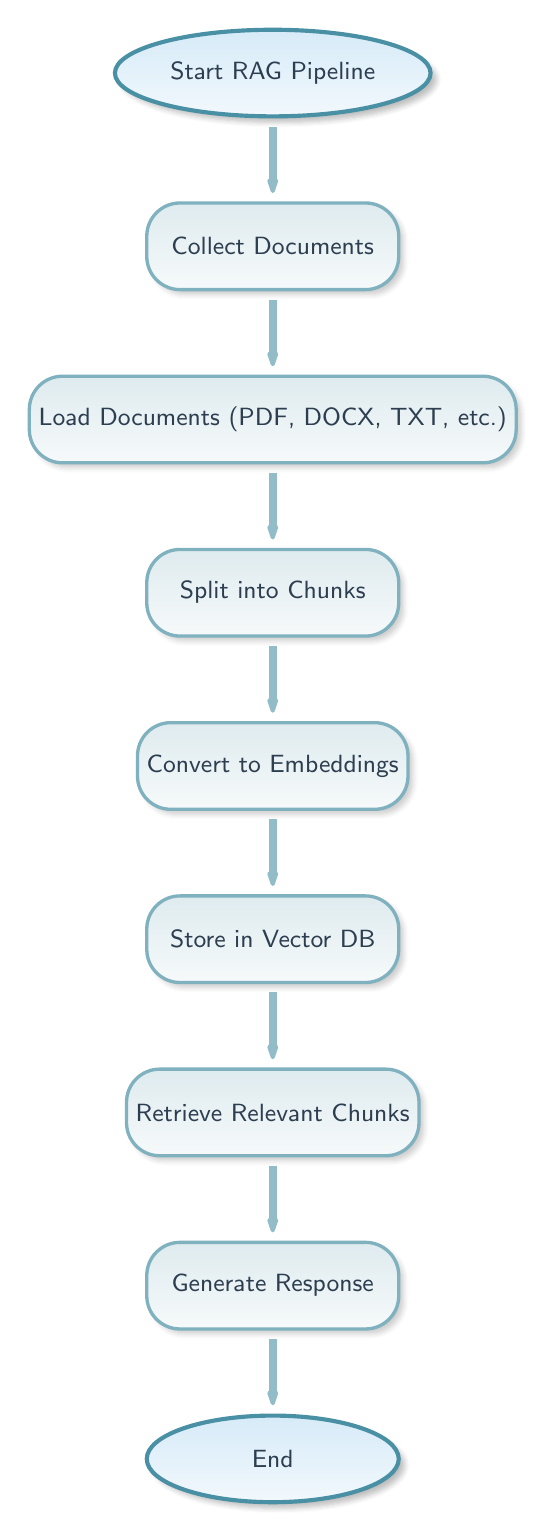
\begin{tikzpicture}[node distance=2.2cm, font=\sffamily\small]
    \node (start) [startstop] {Start RAG Pipeline};
    \node (collect) [process, below of=start] {Collect Documents};
    \node (load) [process, below of=collect] {Load Documents (PDF, DOCX, TXT, etc.)};
    \node (split) [process, below of=load] {Split into Chunks};
    \node (embed) [process, below of=split] {Convert to Embeddings};
    \node (store) [process, below of=embed] {Store in Vector DB};
    \node (retrieve) [process, below of=store] {Retrieve Relevant Chunks};
    \node (generate) [process, below of=retrieve] {Generate Response};
    \node (end) [startstop, below of=generate] {End};

    \draw [arrow] (start) -- (collect);
    \draw [arrow] (collect) -- (load);
    \draw [arrow] (load) -- (split);
    \draw [arrow] (split) -- (embed);
    \draw [arrow] (embed) -- (store);
    \draw [arrow] (store) -- (retrieve);
    \draw [arrow] (retrieve) -- (generate);
    \draw [arrow] (generate) -- (end);
\end{tikzpicture}

\section{Ollama Equivalent Code}
\begin{lstlisting}[language=Python]
# In a RAG pipeline you must:

# 1. Collect documents (PDFs, text files, DOCX, website pages, database rows, etc.)


# 2. Load them into your program


# 3. Split them into chunks


# 4. Convert them into embeddings


# 5. Store them in a vector database



# Here we focus on Step 2 -- Loading documents.


# ---

# Most Common Ways to Load Documents for RAG

# Here are the most frequently used loaders in Python (LangChain):


# ---

# Load PDFs

# Using LangChain's PyPDFLoader

from langchain_community.document_loaders import PyPDFLoader

loader = PyPDFLoader("sample.pdf")
documents = loader.load()

print(documents)




# Load DOCX / Word files

from langchain_community.document_loaders import Docx2txtLoader

loader = Docx2txtLoader("sample.docx")
documents = loader.load()



# Load Text Files (.txt)

from langchain_community.document_loaders import TextLoader

loader = TextLoader("notes.txt")
documents = loader.load()


# Load Multiple Documents in a Folder

from langchain_community.document_loaders import DirectoryLoader

loader = DirectoryLoader(
    "data/",
    glob="*/.pdf",
    show_progress=True
)

documents = loader.load()


# Load Website Pages (HTML)

from langchain_community.document_loaders import WebBaseLoader

loader = WebBaseLoader("http://shooliniuniversity.com/")
documents = loader.load()


# Load Markdown Files (.md)

from langchain_community.document_loaders import UnstructuredMarkdownLoader

loader = UnstructuredMarkdownLoader("readme.md")
documents = loader.load()


# Load CSV Files

from langchain_community.document_loaders.csv_loader import CSVLoader

loader = CSVLoader("data.csv")
documents = loader.load()

loader = CSVLoader("data.csv")
documents = loader.load()
\end{lstlisting}

\subsection{Diff Explanation}
\begin{removedcode}
\begin{diffverb}
- from langchain.document_loaders import PyPDFLoader
- from langchain.document_loaders import Docx2txtLoader
- from langchain.document_loaders import TextLoader
- from langchain.document_loaders import DirectoryLoader
- from langchain.document_loaders import WebBaseLoader
- from langchain.document_loaders import UnstructuredMarkdownLoader
- from langchain.document_loaders.csv_loader import CSVLoader
\end{diffverb}
\end{removedcode}

\begin{addedcode}
\begin{diffverb}
+ from langchain_community.document_loaders import PyPDFLoader
+ from langchain_community.document_loaders import Docx2txtLoader
+ from langchain_community.document_loaders import TextLoader
+ from langchain_community.document_loaders import DirectoryLoader
+ from langchain_community.document_loaders import WebBaseLoader
+ from langchain_community.document_loaders import UnstructuredMarkdownLoader
+ from langchain_community.document_loaders.csv_loader import CSVLoader
\end{diffverb}
\end{addedcode}


\subsection{Explanation of the Diff}
\begin{itemize}
    \item \textbf{Changed import paths:} From \texttt{langchain.document\_loaders} to\\ \texttt{langchain\_community.document\_loaders}.
    \item \textbf{Why:} In newer LangChain versions, community-contributed loaders are moved to the \texttt{langchain\_community} package for better organization.
\end{itemize}

\section{Hugging Face Equivalent Code}
\begin{lstlisting}[language=Python]
# In a RAG pipeline you must:

# 1. Collect documents (PDFs, text files, DOCX, website pages, database rows, etc.)


# 2. Load them into your program


# 3. Split them into chunks


# 4. Convert them into embeddings


# 5. Store them in a vector database



# Here we focus on Step 2 -- Loading documents.


# ---

# Most Common Ways to Load Documents for RAG

# Here are the most frequently used loaders in Python (LangChain):


# ---

# Load PDFs

# Using LangChain's PyPDFLoader

from langchain_community.document_loaders import PyPDFLoader

loader = PyPDFLoader("sample.pdf")
documents = loader.load()

print(documents)




# Load DOCX / Word files

from langchain_community.document_loaders import Docx2txtLoader

loader = Docx2txtLoader("sample.docx")
documents = loader.load()



# Load Text Files (.txt)

from langchain_community.document_loaders import TextLoader

loader = TextLoader("notes.txt")
documents = loader.load()


# Load Multiple Documents in a Folder

from langchain_community.document_loaders import DirectoryLoader

loader = DirectoryLoader(
    "data/",
    glob="*/.pdf",
    show_progress=True
)

documents = loader.load()


# Load Website Pages (HTML)

from langchain_community.document_loaders import WebBaseLoader

loader = WebBaseLoader("http://shooliniuniversity.com/")
documents = loader.load()


# Load Markdown Files (.md)

from langchain_community.document_loaders import UnstructuredMarkdownLoader

loader = UnstructuredMarkdownLoader("readme.md")
documents = loader.load()


# Load CSV Files

from langchain_community.document_loaders.csv_loader import CSVLoader

loader = CSVLoader("data.csv")
documents = loader.load()

loader = CSVLoader("data.csv")
documents = loader.load()
\end{lstlisting}

\subsection{Diff Explanation}
Same as Ollama: Changed import paths to langchain\_community.

\subsection{Explanation of the Diff}
Same as Ollama.


% ===== CODE13 =====
\newpage
\section{Original Code: code13.py}
\begin{lstlisting}[language=Python]
from langchain.document_loaders import TextLoader


path='ipl.txt'

def load_doc(path):
  if path.endswith('.txt'):
    loader=TextLoader(path)
  documents=loader.load()
  return documents

documents=load_doc(path)
print(documents)


# #Now we do chunking as already told model have limit and answer also become accurate

# #1. CharacterTextSplitter

from langchain.text_splitter import CharacterTextSplitter


chunking=CharacterTextSplitter(chunk_size=70,chunk_overlap=39)


docs=chunking.split_documents(documents)

print(len(docs))


for i in range(len(docs)):
    print(docs[i])
    print("------------------------------------------")
\end{lstlisting}

\subsection{Explanation of the Code}
\begin{itemize}
    \item \textbf{What:} This code loads a text file using TextLoader, then splits the document into chunks using CharacterTextSplitter with specified chunk size and overlap, and prints the chunks.
    \item \textbf{Why:} In RAG systems, large documents must be split into manageable chunks to fit model context limits and improve retrieval accuracy. Character-based splitting is simple and preserves some context via overlap.
    \item \textbf{How:}
    \begin{itemize}
        \item Load text file with TextLoader.
        \item Create CharacterTextSplitter with chunk\_size=70 and chunk\_overlap=39.
        \item Split documents into chunks.
        \item Print number of chunks and each chunk.
    \end{itemize}
\end{itemize}

\subsection{Flowchart}
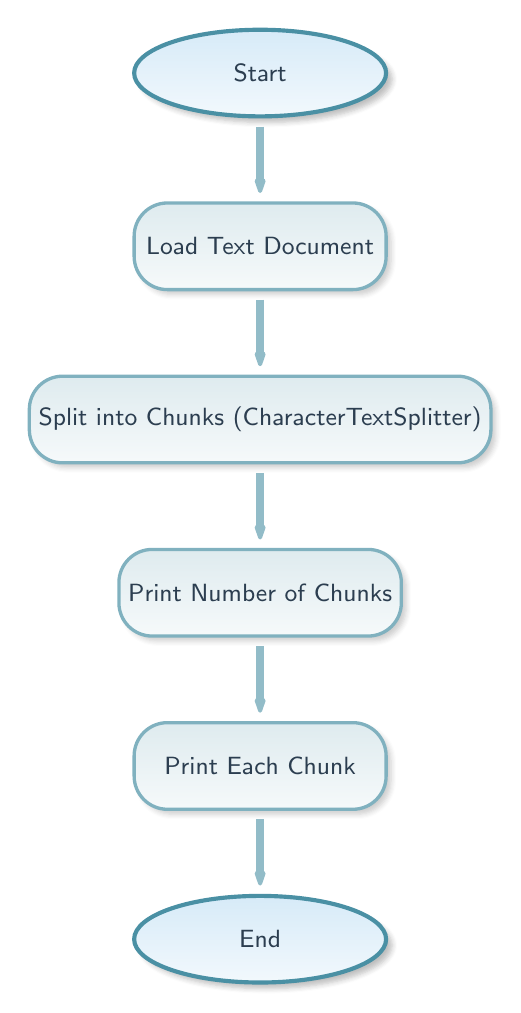
\begin{tikzpicture}[node distance=2.2cm, font=\sffamily\small]
    \node (start) [startstop] {Start};
    \node (load) [process, below of=start] {Load Text Document};
    \node (split) [process, below of=load] {Split into Chunks (CharacterTextSplitter)};
    \node (print_count) [process, below of=split] {Print Number of Chunks};
    \node (print_chunks) [process, below of=print_count] {Print Each Chunk};
    \node (end) [startstop, below of=print_chunks] {End};

    \draw [arrow] (start) -- (load);
    \draw [arrow] (load) -- (split);
    \draw [arrow] (split) -- (print_count);
    \draw [arrow] (print_count) -- (print_chunks);
    \draw [arrow] (print_chunks) -- (end);
\end{tikzpicture}

\section{Ollama Equivalent Code}
\begin{lstlisting}[language=Python]
from langchain_community.document_loaders import TextLoader


path='ipl.txt'

def load_doc(path):
  if path.endswith('.txt'):
    loader=TextLoader(path)
  documents=loader.load()
  return documents

documents=load_doc(path)
print(documents)


# #Now we do chunking as already told model have limit and answer also become accurate

# #1. CharacterTextSplitter

from langchain_text_splitters import CharacterTextSplitter


chunking=CharacterTextSplitter(chunk_size=70,chunk_overlap=39)


docs=chunking.split_documents(documents)

print(len(docs))


for i in range(len(docs)):
    print(docs[i])
    print("------------------------------------------")
\end{lstlisting}

\subsection{Diff Explanation}
\begin{removedcode}
\begin{diffverb}
- from langchain.document_loaders import TextLoader
- from langchain.text_splitter import CharacterTextSplitter
\end{diffverb}
\end{removedcode}

\begin{addedcode}
\begin{diffverb}
+ from langchain_community.document_loaders import TextLoader
+ from langchain_text_splitters import CharacterTextSplitter
\end{diffverb}
\end{addedcode}


\subsection{Explanation of the Diff}
\begin{itemize}
    \item \textbf{Changed import paths:} Loaders to langchain\_community, splitters to langchain\_text\_splitters.
    \item \textbf{Why:} Modularization in newer LangChain versions.
\end{itemize}

\section{Hugging Face Equivalent Code}
Same as Ollama.

\subsection{Diff Explanation}
Same as Ollama.


% ===== CODE13A =====
\newpage
\section{Original Code: code13A.py}
\begin{lstlisting}[language=Python]
from langchain.document_loaders import TextLoader


path='ipl.txt'

def load_doc(path):
  if path.endswith('.txt'):
    loader=TextLoader(path)
  documents=loader.load()
  return documents

documents=load_doc(path)
print(documents)


# #Now we do chunking as already told model have limit and answer also become accurate


import os
from langchain_openai import AzureOpenAIEmbeddings


AZURE_OPENAI_API_KEY = ""  #Put your own API key
AZURE_OPENAI_ENDPOINT = "https://chatgpt-key.openai.azure.com/"
AZURE_OPENAI_DEPLOYMENT_NAME = "gpt-4o-2"
AZURE_OPENAI_API_VERSION = "2025-01-01-preview"
AZURE_OPENAI_EMBEDDING_DEPLOYMENT_NAME = "text-embedding-3-large" # Replace with your embedding deployment name
AZURE_OPENAI_EMBEDDING_MODEL_NAME = "text-embedding-3-large" # Replace with your embedding model name


embeddings = AzureOpenAIEmbeddings(
    deployment=AZURE_OPENAI_EMBEDDING_DEPLOYMENT_NAME,
    model=AZURE_OPENAI_EMBEDDING_MODEL_NAME,
    api_key=AZURE_OPENAI_API_KEY,
    azure_endpoint=AZURE_OPENAI_ENDPOINT,
    api_version=AZURE_OPENAI_API_VERSION,
)


from langchain_experimental.text_splitter import SemanticChunker
from langchain_openai import OpenAIEmbeddings


chunker = SemanticChunker(embeddings)
chunks = chunker.create_documents([documents])

for c in chunks:
    print(c.page_content)
\end{lstlisting}

\subsection{Explanation of the Code}
\begin{itemize}
    \item \textbf{What:} This code loads a text file, initializes Azure OpenAI embeddings, and uses SemanticChunker to split the document into semantically coherent chunks based on embeddings.
    \item \textbf{Why:} Semantic chunking groups text by meaning rather than fixed characters, leading to better retrieval in RAG as chunks maintain topical coherence. Uses embeddings to determine split points.
    \item \textbf{How:}
    \begin{itemize}
        \item Load text document.
        \item Set up Azure OpenAI embeddings with API details.
        \item Create SemanticChunker with embeddings.
        \item Generate chunks from documents.
        \item Print each chunk's content.
    \end{itemize}
\end{itemize}

\subsection{Flowchart}
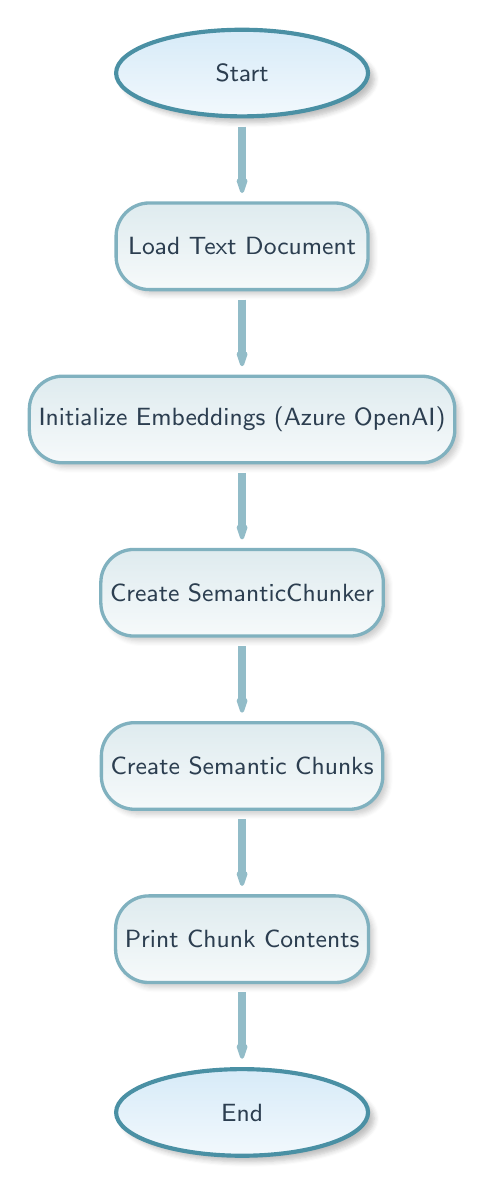
\begin{tikzpicture}[node distance=2.2cm, font=\sffamily\small]
    \node (start) [startstop] {Start};
    \node (load) [process, below of=start] {Load Text Document};
    \node (init_embed) [process, below of=load] {Initialize Embeddings (Azure OpenAI)};
    \node (create_chunker) [process, below of=init_embed] {Create SemanticChunker};
    \node (chunk) [process, below of=create_chunker] {Create Semantic Chunks};
    \node (print) [process, below of=chunk] {Print Chunk Contents};
    \node (end) [startstop, below of=print] {End};

    \draw [arrow] (start) -- (load);
    \draw [arrow] (load) -- (init_embed);
    \draw [arrow] (init_embed) -- (create_chunker);
    \draw [arrow] (create_chunker) -- (chunk);
    \draw [arrow] (chunk) -- (print);
    \draw [arrow] (print) -- (end);
\end{tikzpicture}

\section{Ollama Equivalent Code}
\begin{lstlisting}[language=Python]
from langchain_community.document_loaders import TextLoader


path='ipl.txt'

def load_doc(path):
  if path.endswith('.txt'):
    loader=TextLoader(path)
  documents=loader.load()
  return documents

documents=load_doc(path)
print(documents)


# #Now we do chunking as already told model have limit and answer also become accurate


from langchain_community.embeddings import HuggingFaceEmbeddings


embeddings = HuggingFaceEmbeddings(model_name="BAAI/bge-m3")


from langchain_experimental.text_splitter import SemanticChunker


chunker = SemanticChunker(embeddings)
chunks = chunker.create_documents([documents])

for c in chunks:
    print(c.page_content)
\end{lstlisting}

\subsection{Diff Explanation}
\begin{removedcode}
\begin{diffverb}
- from langchain.document_loaders import TextLoader
- import os
- from langchain_openai import AzureOpenAIEmbeddings
- AZURE_OPENAI_API_KEY = "" ... (Azure setup)
- embeddings = AzureOpenAIEmbeddings(...)
- from langchain_experimental.text_splitter import SemanticChunker
- from langchain_openai import OpenAIEmbeddings
\end{diffverb}
\end{removedcode}

\begin{addedcode}
\begin{diffverb}
+ from langchain_community.document_loaders import TextLoader
+ from langchain_community.embeddings import HuggingFaceEmbeddings
+ embeddings = HuggingFaceEmbeddings(model_name="BAAI/bge-m3")
+ from langchain_experimental.text_splitter import SemanticChunker
\end{diffverb}
\end{addedcode}


\subsection{Explanation of the Diff}
\begin{itemize}
    \item \textbf{Removed Azure embeddings:} Replaced with local HuggingFace embeddings.
    \item \textbf{Changed imports:} To langchain\_community.
    \item \textbf{Why:} Adapts to local embeddings for Ollama, avoiding cloud API costs.
\end{itemize}

\section{Hugging Face Equivalent Code}
Same as Ollama.

\subsection{Diff Explanation}
Same as Ollama.


% ===== CODE14 =====
\newpage
\section{Original Code: code14.py}
\begin{lstlisting}[language=Python]
import os
from langchain_openai import AzureOpenAIEmbeddings

AZURE_OPENAI_API_KEY = ""  #Put your own API key
AZURE_OPENAI_ENDPOINT = "https://chatgpt-key.openai.azure.com/"
AZURE_OPENAI_DEPLOYMENT_NAME = "gpt-4o-2"
AZURE_OPENAI_API_VERSION = "2025-01-01-preview"
AZURE_OPENAI_EMBEDDING_DEPLOYMENT_NAME = "text-embedding-3-large" # Replace with your embedding deployment name
AZURE_OPENAI_EMBEDDING_MODEL_NAME = "text-embedding-3-large" # Replace with your embedding model name


embeddings = AzureOpenAIEmbeddings(
    deployment=AZURE_OPENAI_EMBEDDING_DEPLOYMENT_NAME,
    model=AZURE_OPENAI_EMBEDDING_MODEL_NAME,
    api_key=AZURE_OPENAI_API_KEY,
    azure_endpoint=AZURE_OPENAI_ENDPOINT,
    api_version=AZURE_OPENAI_API_VERSION,
)

text = "I love machine learning"


embedding = embeddings.embed_query(text)

print(f"Embedding vector length: {len(embedding)}")
print(embedding)
\end{lstlisting}

\subsection{Explanation of the Code}
\begin{itemize}
    \item \textbf{What:} This code initializes Azure OpenAI embeddings and generates an embedding vector for the text "I love machine learning", then prints the vector length and the vector.
    \item \textbf{Why:} Embeddings convert text into numerical vectors for semantic similarity in RAG systems. Azure provides high-quality embeddings via API.
    \item \textbf{How:}
    \begin{itemize}
        \item Set up Azure OpenAI embeddings with API details.
        \item Call embed\_query on the text.
        \item Print length and vector.
    \end{itemize}
\end{itemize}

\subsection{Flowchart}
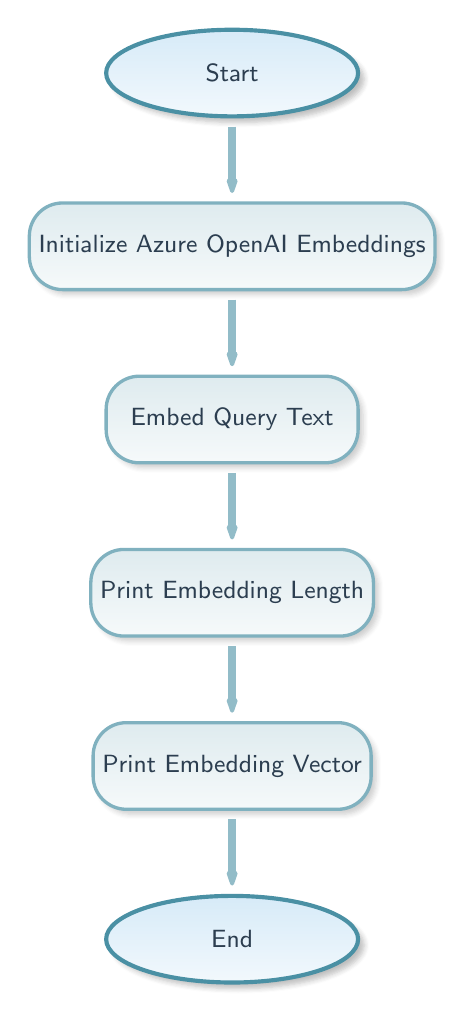
\begin{tikzpicture}[node distance=2.2cm, font=\sffamily\small]
    \node (start) [startstop] {Start};
    \node (init_embed) [process, below of=start] {Initialize Azure OpenAI Embeddings};
    \node (embed) [process, below of=init_embed] {Embed Query Text};
    \node (print_len) [process, below of=embed] {Print Embedding Length};
    \node (print_vec) [process, below of=print_len] {Print Embedding Vector};
    \node (end) [startstop, below of=print_vec] {End};

    \draw [arrow] (start) -- (init_embed);
    \draw [arrow] (init_embed) -- (embed);
    \draw [arrow] (embed) -- (print_len);
    \draw [arrow] (print_len) -- (print_vec);
    \draw [arrow] (print_vec) -- (end);
\end{tikzpicture}

\section{Ollama Equivalent Code}
\begin{lstlisting}[language=Python]
from langchain_community.embeddings import HuggingFaceEmbeddings

embedding_model = HuggingFaceEmbeddings(model_name="BAAI/bge-m3")

text = "I love machine learning"

embedding = embedding_model.embed_query(text)

print(f"Embedding vector length: {len(embedding)}")
print(embedding)
\end{lstlisting}

\subsection{Diff Explanation}
\begin{removedcode}
\begin{diffverb}
- import os
- from langchain_openai import AzureOpenAIEmbeddings
- AZURE_OPENAI_API_KEY = "" ... (Azure setup)
- embeddings = AzureOpenAIEmbeddings(...)
\end{diffverb}
\end{removedcode}

\begin{addedcode}
\begin{diffverb}
+ from langchain_community.embeddings import HuggingFaceEmbeddings
+ embedding_model = HuggingFaceEmbeddings(model_name="BAAI/bge-m3")
\end{diffverb}
\end{addedcode}


\subsection{Explanation of the Diff}
\begin{itemize}
    \item \textbf{Removed Azure setup:} Local embeddings.
    \item \textbf{Changed to HuggingFace:} Uses BAAI/bge-m3 model.
    \item \textbf{Why:} Local execution without API keys.
\end{itemize}

\section{Hugging Face Equivalent Code}
\begin{lstlisting}[language=Python]
from FlagEmbedding import BGEM3FlagModel

model=BGEM3FlagModel('BAAI/bge-m3',use_fp16=True)

sentence1="I love machine learning"

embeddings1=model.encode(sentence1,
                        batch_size=12,
                        max_length=8192,)['dense_vecs']

print(embeddings1)
\end{lstlisting}

\subsection{Diff Explanation}
\begin{removedcode}
\begin{diffverb}
- from langchain_community.embeddings import HuggingFaceEmbeddings
- embedding_model = HuggingFaceEmbeddings(model_name="BAAI/bge-m3")
- embedding = embedding_model.embed_query(text)
- print(f"Embedding vector length: {len(embedding)}")
- print(embedding)
\end{diffverb}
\end{removedcode}

\begin{addedcode}
\begin{diffverb}
+ from FlagEmbedding import BGEM3FlagModel
+ model=BGEM3FlagModel('BAAI/bge-m3',use_fp16=True)
+ sentence1="I love machine learning"
+ embeddings1=model.encode(sentence1, batch_size=12, max_length=8192,)['dense_vecs']
+ print(embeddings1)
\end{diffverb}
\end{addedcode}


\subsection{Explanation of the Diff}
\begin{itemize}
    \item \textbf{Removed LangChain wrapper:} Direct FlagEmbedding usage.
    \item \textbf{Changed method:} encode instead of embed\_query.
    \item \textbf{Why:} Direct access to Hugging Face embedding models for more control.
\end{itemize}


% ===== CODE14A =====
\newpage
\section{Original Code: code14A.py}
\begin{lstlisting}[language=Python]
# !pip install -U FlagEmbedding

from FlagEmbedding import BGEM3FlagModel

model=BGEM3FlagModel('BAAI/bge-m3',use_fp16=True)

sentence1="I am going to school"

embeddings1=model.encode(sentence1,
                        batch_size=12,
                        max_length=8192,)['dense_vecs']

print(embeddings1)
\end{lstlisting}

\subsection{Explanation of the Code}
\begin{itemize}
    \item \textbf{What:} This code loads the BGE-M3 embedding model from FlagEmbedding and generates dense embeddings for the sentence "I am going to school", then prints the embedding vector.
    \item \textbf{Why:} Direct use of advanced embedding models for text representation. BGE-M3 is a state-of-the-art model for semantic embeddings.
    \item \textbf{How:}
    \begin{itemize}
        \item Install FlagEmbedding if needed.
        \item Initialize BGEM3FlagModel with model name and fp16.
        \item Encode the sentence with parameters.
        \item Extract and print dense vectors.
    \end{itemize}
\end{itemize}

\subsection{Flowchart}
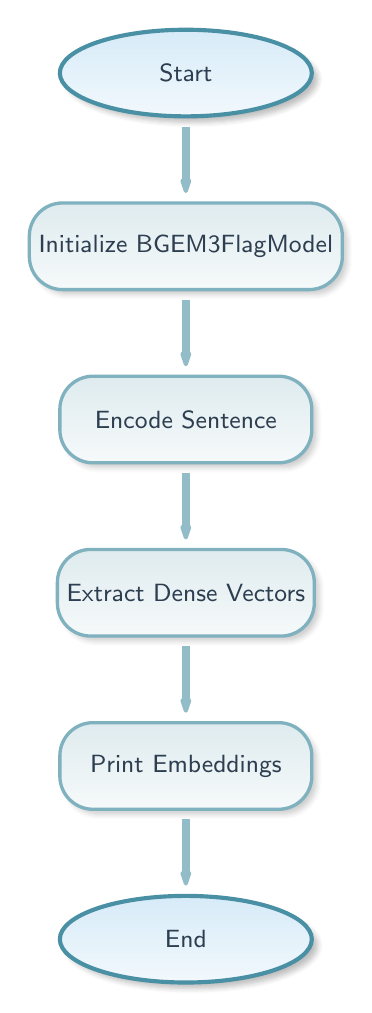
\begin{tikzpicture}[node distance=2.2cm, font=\sffamily\small]
    \node (start) [startstop] {Start};
    \node (init_model) [process, below of=start] {Initialize BGEM3FlagModel};
    \node (encode) [process, below of=init_model] {Encode Sentence};
    \node (extract) [process, below of=encode] {Extract Dense Vectors};
    \node (print) [process, below of=extract] {Print Embeddings};
    \node (end) [startstop, below of=print] {End};

    \draw [arrow] (start) -- (init_model);
    \draw [arrow] (init_model) -- (encode);
    \draw [arrow] (encode) -- (extract);
    \draw [arrow] (extract) -- (print);
    \draw [arrow] (print) -- (end);
\end{tikzpicture}

\section{Ollama Equivalent Code}
Same as original.

\subsection{Diff Explanation}
No changes.

\subsection{Explanation of the Diff}
All versions use the same direct FlagEmbedding approach.

\section{Hugging Face Equivalent Code}
Same as original.

\subsection{Diff Explanation}
No changes.


% ===== CODE15 =====
\newpage
\section{Original Code (src/code15.py)}

The original code demonstrates computing cosine similarity between two sentences using the BGEM3FlagModel from FlagEmbedding.

\begin{lstlisting}[language=Python]
#cosine similarity


# !pip install -U FlagEmbedding

from FlagEmbedding import BGEM3FlagModel
from sklearn.metrics.pairwise import cosine_similarity

model=BGEM3FlagModel('BAAI/bge-m3',use_fp16=True)

sentence1="I am going to school"

embeddings1=model.encode(sentence1,
                        batch_size=12,
                        max_length=8192,)['dense_vecs']

print(embeddings1)

sentence2="I am going to home"

embeddings2=model.encode(sentence2,
                        batch_size=12,
                        max_length=8192,)['dense_vecs']

print(embeddings2)

similiarity_list= cosine_similarity(
      [embeddings1],
      [embeddings2]
  )[0][0]

print(similarity)
\end{lstlisting}

\section{Explanation}

\subsection{What}
This code computes the cosine similarity between the embeddings of two sentences. Cosine similarity measures the cosine of the angle between two vectors in a multi-dimensional space, providing a value between -1 and 1 that indicates how similar the vectors (and thus the sentences) are semantically.

\subsection{Why}
Sentence embeddings represent the semantic meaning of text in a numerical vector form. By comparing these vectors using cosine similarity, we can quantify how closely related two pieces of text are. This is useful in applications like semantic search, text clustering, and recommendation systems where understanding textual similarity is key.

\subsection{How}
1. Import the BGEM3FlagModel from FlagEmbedding and cosine\_similarity from sklearn.
2. Initialize the model with the 'BAAI/bge-m3' pre-trained model, enabling FP16 for efficiency.
3. Encode two sentences into dense vector embeddings using the model's encode method, specifying batch size and max length.
4. Compute the cosine similarity between the two embedding vectors.
5. Print the embeddings and the similarity score.

Note: There is a typo in the code: 'similiarity\_list' should be 'similarity', and 'print(similarity)' at the end.

\section{Flowchart}

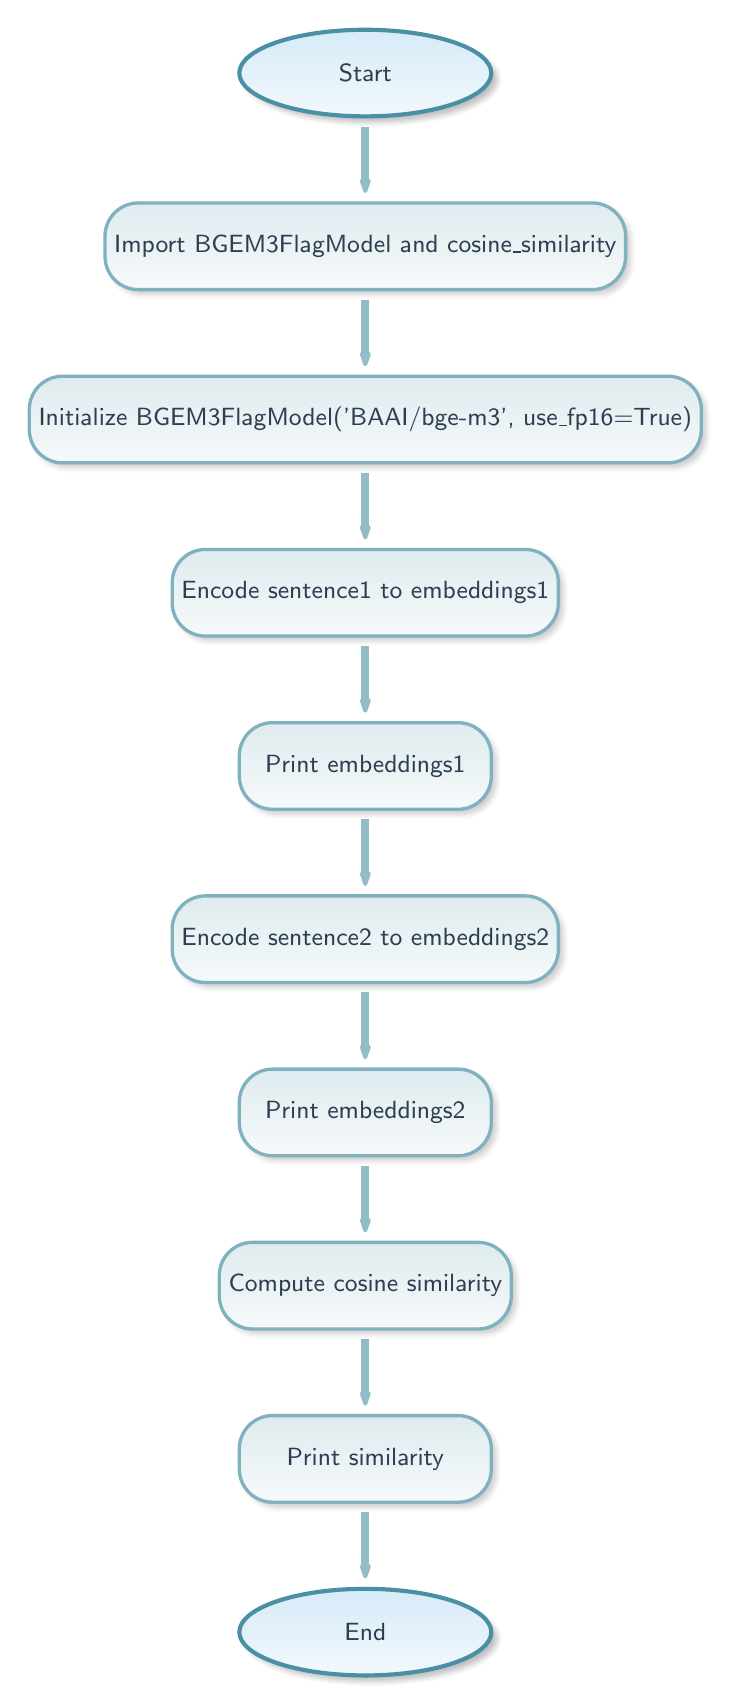
\begin{tikzpicture}[node distance=2.2cm, font=\sffamily\small]
    \node (start) [startstop] {Start};
    \node (import) [process, below of=start] {Import BGEM3FlagModel and cosine\_similarity};
    \node (init) [process, below of=import] {Initialize BGEM3FlagModel('BAAI/bge-m3', use\_fp16=True)};
    \node (encode1) [process, below of=init] {Encode sentence1 to embeddings1};
    \node (print1) [process, below of=encode1] {Print embeddings1};
    \node (encode2) [process, below of=print1] {Encode sentence2 to embeddings2};
    \node (print2) [process, below of=encode2] {Print embeddings2};
    \node (compute) [process, below of=print2] {Compute cosine similarity};
    \node (print3) [process, below of=compute] {Print similarity};
    \node (end) [startstop, below of=print3] {End};

    \draw [arrow] (start) -- (import);
    \draw [arrow] (import) -- (init);
    \draw [arrow] (init) -- (encode1);
    \draw [arrow] (encode1) -- (print1);
    \draw [arrow] (print1) -- (encode2);
    \draw [arrow] (encode2) -- (print2);
    \draw [arrow] (print2) -- (compute);
    \draw [arrow] (compute) -- (print3);
    \draw [arrow] (print3) -- (end);
\end{tikzpicture}


% ===== CODE15A =====
\newpage
\section{Original Code (src/code15A.py)}

The original code demonstrates computing cosine similarity between embeddings of a text document and a query using Azure OpenAI Embeddings.

\begin{lstlisting}[language=Python]
from langchain_openai import AzureOpenAIEmbeddings
import os

embedding_model = AzureOpenAIEmbeddings(
    openai_api_key="",
    azure_deployment="text-embedding-3-large",
    azure_endpoint="https://chatgpt-key.openai.azure.com",
    openai_api_type="azure",
    openai_api_version="2023-05-15",
    chunk_size=1000
)


text ='''
Marwadi University (MU)[1] is a private university[2] located in Rajkot, Gujarat, India. It was established on 9 May 2016 by the Marwadi Education Foundation through The Gujarat Private Universities (Amendment) Act, 2016.[3] As of 2017, it offers 54 different courses.[4] It is graded A+ by NAAC.[5]

The university operates under the division of Marwadi Education Foundation's Group of Institutions (MEFGI). MEFGI commenced its operations in the year 2008. It was established as a primary unit of Marwadi Education Foundation under the Bombay Public Trust Act 1950. Marwadi University is aided by the Marwadi Shares and Finance Limited, a stock broking company in India and Chandarana Intermediaries Brokers Pvt. Ltd. (CIBPL), a firm dealing in technical and arbitrage trading.[6]

Campus
The campus is located on 52 acres of land, having a distance of nearly 40 minutes from railway and airports. The university comprises eight multi-storey buildings.[7] Laboratories, research facilities, student clubs, sports club and college cafeteria are available.[8]

There are two libraries with RFID technologies, 60+ computer systems, 50000+ books.[9] The campus also includes banking and ATM facilities.[10] Around 70+ buses function every day at regular intervals for students and staff.[11] There are hostel rooms with internet facilities, laundry, dance rooms, libraries etc. and capacity to occupy over 2000 students.[12]

'''


query="What is shoolini University?"




embedding_text = embedding_model.embed_query(text)

embedding_query = embedding_model.embed_query(query)


from sklearn.metrics.pairwise import cosine_similarity




sim = cosine_similarity(
    [embeddings_query],   # query embedding
    [embedding_text]       # document embedding
)[0][0]



print(f"Embedding vector length: {len(embedding)}")
print(embedding_text)
print("---------------------------------------------------------------------")
print(f"Embedding vector length: {len(embedding_query)}")
print(sim)
\end{lstlisting}

\section{Explanation}

\subsection{What}
This code computes the cosine similarity between the embeddings of a long text document (about Marwadi University) and a query string using Azure OpenAI's text-embedding-3-large model. It demonstrates how to use cloud-based embeddings for semantic similarity measurement.

\subsection{Why}
Embeddings from large language models like OpenAI's can capture rich semantic information. Cosine similarity on these embeddings allows quantifying how relevant a document is to a query, which is fundamental for information retrieval, question-answering systems, and RAG (Retrieval-Augmented Generation) pipelines.

\subsection{How}
1. Import AzureOpenAIEmbeddings from langchain\_openai and cosine\_similarity from sklearn.
2. Initialize the embedding model with Azure OpenAI credentials and configuration (deployment, endpoint, API version, chunk size).
3. Define a long text document and a query.
4. Embed both the text and query using the model's embed\_query method.
5. Compute cosine similarity between the query and text embeddings.
6. Print the embedding vector lengths, the text embedding, and the similarity score.

Note: There are typos in the code: 'embeddings\_query' should be 'embedding\_query', and 'len(embedding)' should be 'len(embedding\_text)'.

\section{Flowchart}

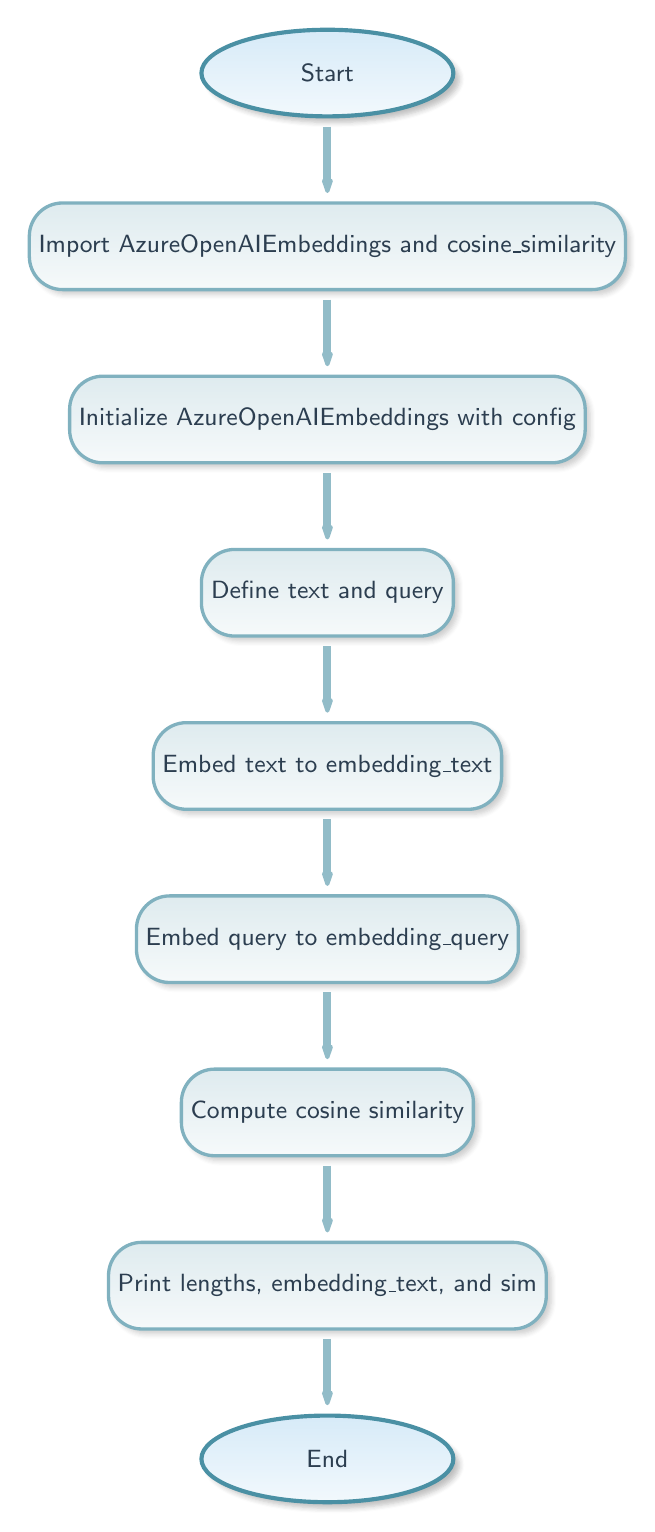
\begin{tikzpicture}[node distance=2.2cm, font=\sffamily\small]
    \node (start) [startstop] {Start};
    \node (import) [process, below of=start] {Import AzureOpenAIEmbeddings and cosine\_similarity};
    \node (init) [process, below of=import] {Initialize AzureOpenAIEmbeddings with config};
    \node (define) [process, below of=init] {Define text and query};
    \node (embed_text) [process, below of=define] {Embed text to embedding\_text};
    \node (embed_query) [process, below of=embed_text] {Embed query to embedding\_query};
    \node (compute) [process, below of=embed_query] {Compute cosine similarity};
    \node (print) [process, below of=compute] {Print lengths, embedding\_text, and sim};
    \node (end) [startstop, below of=print] {End};

    \draw [arrow] (start) -- (import);
    \draw [arrow] (import) -- (init);
    \draw [arrow] (init) -- (define);
    \draw [arrow] (define) -- (embed_text);
    \draw [arrow] (embed_text) -- (embed_query);
    \draw [arrow] (embed_query) -- (compute);
    \draw [arrow] (compute) -- (print);
    \draw [arrow] (print) -- (end);
\end{tikzpicture}

\section{Ollama Equivalent Code}

\begin{lstlisting}[language=Python]
from langchain_community.embeddings import HuggingFaceEmbeddings
from sklearn.metrics.pairwise import cosine_similarity

embedding_model = HuggingFaceEmbeddings(model_name='BAAI/bge-m3')

text ='''
Marwadi University (MU)[1] is a private university[2] located in Rajkot, Gujarat, India. It was established on 9 May 2016 by the Marwadi Education Foundation through The Gujarat Private Universities (Amendment) Act, 2016.[3] As of 2017, it offers 54 different courses.[4] It is graded A+ by NAAC.[5]

The university operates under the division of Marwadi Education Foundation's Group of Institutions (MEFGI). MEFGI commenced its operations in the year 2008. It was established as a primary unit of Marwadi Education Foundation under the Bombay Public Trust Act 1950. Marwadi University is aided by the Marwadi Shares and Finance Limited, a stock broking company in India and Chandarana Intermediaries Brokers Pvt. Ltd. (CIBPL), a firm dealing in technical and arbitrage trading.[6]

Campus
The campus is located on 52 acres of land, having a distance of nearly 40 minutes from railway and airports. The university comprises eight multi-storey buildings.[7] Laboratories, research facilities, student clubs, sports club and college cafeteria are available.[8]

There are two libraries with RFID technologies, 60+ computer systems, 50000+ books.[9] The campus also includes banking and ATM facilities.[10] Around 70+ buses function every day at regular intervals for students and staff.[11] There are hostel rooms with internet facilities, laundry, dance rooms, libraries etc. and capacity to occupy over 2000 students.[12]

'''

query="What is shoolini University?"

embedding_text = embedding_model.embed_query(text)

embedding_query = embedding_model.embed_query(query)

sim = cosine_similarity(
    [embedding_query],   # query embedding
    [embedding_text]       # document embedding
)[0][0]

print(f"Embedding vector length: {len(embedding_text)}")
print(embedding_text)
print("---------------------------------------------------------------------")
print(f"Embedding vector length: {len(embedding_query)}")
print(sim)
\end{lstlisting}

\subsection{Diff Explanation}

The Ollama equivalent uses LangChain's HuggingFaceEmbeddings with a local BGE-M3 model instead of Azure OpenAI, and fixes the variable name typos.

Key changes:
\begin{itemize}
    \item \textcolor{red}{Removed:} \texttt{from langchain\_openai import AzureOpenAIEmbeddings}
    \item \textcolor{green}{Added:} \texttt{from langchain\_community.embeddings import HuggingFaceEmbeddings}
    \item \textcolor{red}{Removed:} AzureOpenAIEmbeddings initialization with API keys
    \item \textcolor{green}{Added:} \texttt{embedding\_model = HuggingFaceEmbeddings(model\_name='BAAI/bge-m3')}
    \item \textcolor{green}{Fixed:} \texttt{[embedding\_query]} instead of \texttt{[embeddings\_query]}
    \item \textcolor{green}{Fixed:} \texttt{len(embedding\_text)} instead of \texttt{len(embedding)}
\end{itemize}

These changes replace cloud-based embeddings with local, open-source ones for privacy and cost reasons, while maintaining the same similarity computation logic.

\section{Hugging Face Equivalent Code}

\begin{lstlisting}[language=Python]
from FlagEmbedding import BGEM3FlagModel
from sklearn.metrics.pairwise import cosine_similarity

embedding_model = BGEM3FlagModel('BAAI/bge-m3', use_fp16=True)

text ='''
Marwadi University (MU)[1] is a private university[2] located in Rajkot, Gujarat, India. It was established on 9 May 2016 by the Marwadi Education Foundation through The Gujarat Private Universities (Amendment) Act, 2016.[3] As of 2017, it offers 54 different courses.[4] It is graded A+ by NAAC.[5]

The university operates under the division of Marwadi Education Foundation's Group of Institutions (MEFGI). MEFGI commenced its operations in the year 2008. It was established as a primary unit of Marwadi Education Foundation under the Bombay Public Trust Act 1950. Marwadi University is aided by the Marwadi Shares and Finance Limited, a stock broking company in India and Chandarana Intermediaries Brokers Pvt. Ltd. (CIBPL), a firm dealing in technical and arbitrage trading.[6]

Campus
The campus is located on 52 acres of land, having a distance of nearly 40 minutes from railway and airports. The university comprises eight multi-storey buildings.[7] Laboratories, research facilities, student clubs, sports club and college cafeteria are available.[8]

There are two libraries with RFID technologies, 60+ computer systems, 50000+ books.[9] The campus also includes banking and ATM facilities.[10] Around 70+ buses function every day at regular intervals for students and staff.[11] There are hostel rooms with internet facilities, laundry, dance rooms, libraries etc. and capacity to occupy over 2000 students.[12]

'''

query="What is shoolini University?"

embedding_text = embedding_model.encode(text, batch_size=12, max_length=8192)['dense_vecs']

embedding_query = embedding_model.encode(query, batch_size=12, max_length=8192)['dense_vecs']

sim = cosine_similarity(
    [embedding_query],   # query embedding
    [embedding_text]       # document embedding
)[0][0]

print(f"Embedding vector length: {len(embedding_text)}")
print(embedding_text)
print("---------------------------------------------------------------------")
print(f"Embedding vector length: {len(embedding_query)}")
print(sim)
\end{lstlisting}

\subsection{Diff Explanation}

The Hugging Face equivalent uses the direct BGEM3FlagModel from FlagEmbedding instead of LangChain wrappers, and uses the encode method with parameters.

Key changes:
\begin{itemize}
    \item \textcolor{red}{Removed:} LangChain HuggingFaceEmbeddings
    \item \textcolor{green}{Added:} \texttt{from FlagEmbedding import BGEM3FlagModel}
    \item \textcolor{red}{Removed:} \texttt{embedding\_model = HuggingFaceEmbeddings(...)}
    \item \textcolor{green}{Added:} \texttt{embedding\_model = BGEM3FlagModel('BAAI/bge-m3', use\_fp16=True)}
    \item \textcolor{red}{Removed:} \texttt{embed\_query} method
    \item \textcolor{green}{Added:} \texttt{encode} method with \texttt{batch\_size} and \texttt{max\_length} parameters
    \item \textcolor{green}{Fixed:} Variable names consistent
\end{itemize}

These changes use the native FlagEmbedding library for more direct control over encoding parameters, suitable for high-performance local inference.


% ===== CODE16 =====
\newpage
\section{Original Code (src/code16.py)}

The original code implements a movie recommendation system based on semantic similarity between user-input genres and movie descriptions using BGEM3FlagModel embeddings.

\begin{lstlisting}[language=Python]
# !pip install -U FlagEmbedding

from FlagEmbedding import BGEM3FlagModel
from sklearn.metrics.pairwise import cosine_similarity

model = BGEM3FlagModel('BAAI/bge-m3', use_fp16=True)


movies_list = [
    "Shadow Hunters: ACTION FANTASY THRILLER",
    "Eternal Bonds: DRAMA ROMANCE FAMILY",
    "Neon Horizon: SCI-FI ACTION ADVENTURE",
    "Whispers in the Dark: HORROR MYSTERY THRILLER",
    "Crimson Crown: HISTORICAL WAR DRAMA",
    "Starlight Dreams: ROMANCE COMEDY MUSIC",
    "Code Breakers: TECH THRILLER CRIME",
    "The Lost Kingdom: ADVENTURE ACTION FANTASY",
    "Broken Silence: CRIME DRAMA SUSPENSE",
    "Frozen Ashes: SURVIVAL DRAMA ACTION"
]

# Convert movie list into embeddings
embeddings_list = []
for movie in movies_list:
    emb = model.encode(
        movie,
        batch_size=12,
        max_length=8192
    )['dense_vecs']
    embeddings_list.append(emb)


query = input("ENTER THE GENRE FOR WHICH YOU WANT TO SEE MOVIES: ")


query_embedding = model.encode(
    query,
    batch_size=12,
    max_length=8192
)['dense_vecs']


similarity_scores = {}

for i, movie_emb in enumerate(embeddings_list):
    similarity = cosine_similarity(
        [query_embedding],
        [movie_emb]
    )[0][0]

    similarity_scores[movies_list[i]] = similarity


sorted_movies = sorted(similarity_scores.items(), key=lambda x: x[1], reverse=True)

#Retrived data
print("\n Top Recommended Movies:")
for movie, score in sorted_movies[:4]:
    print(f"{movie}   ---> Similarity: {score:.4f}")
\end{lstlisting}

\section{Explanation}

\subsection{What}
This code builds a simple movie recommendation system by computing semantic similarity between a user-provided genre query and a list of movie descriptions (including genres). It uses sentence embeddings to find movies whose descriptions are most similar to the query.

\subsection{Why}
Traditional keyword-based search might miss movies with related but not exact genre matches (e.g., "action" vs. "adventure action"). Semantic embeddings capture meaning, allowing recommendations based on conceptual similarity, improving user experience in content discovery.

\subsection{How}
1. Import BGEM3FlagModel and cosine\_similarity.
2. Initialize the embedding model.
3. Define a list of movie descriptions with genres.
4. Embed each movie description into vectors and store in a list.
5. Take user input for a genre query.
6. Embed the query into a vector.
7. Compute cosine similarity between the query embedding and each movie embedding.
8. Sort movies by similarity score descending.
9. Print the top 4 recommended movies with their scores.

\section{Flowchart}

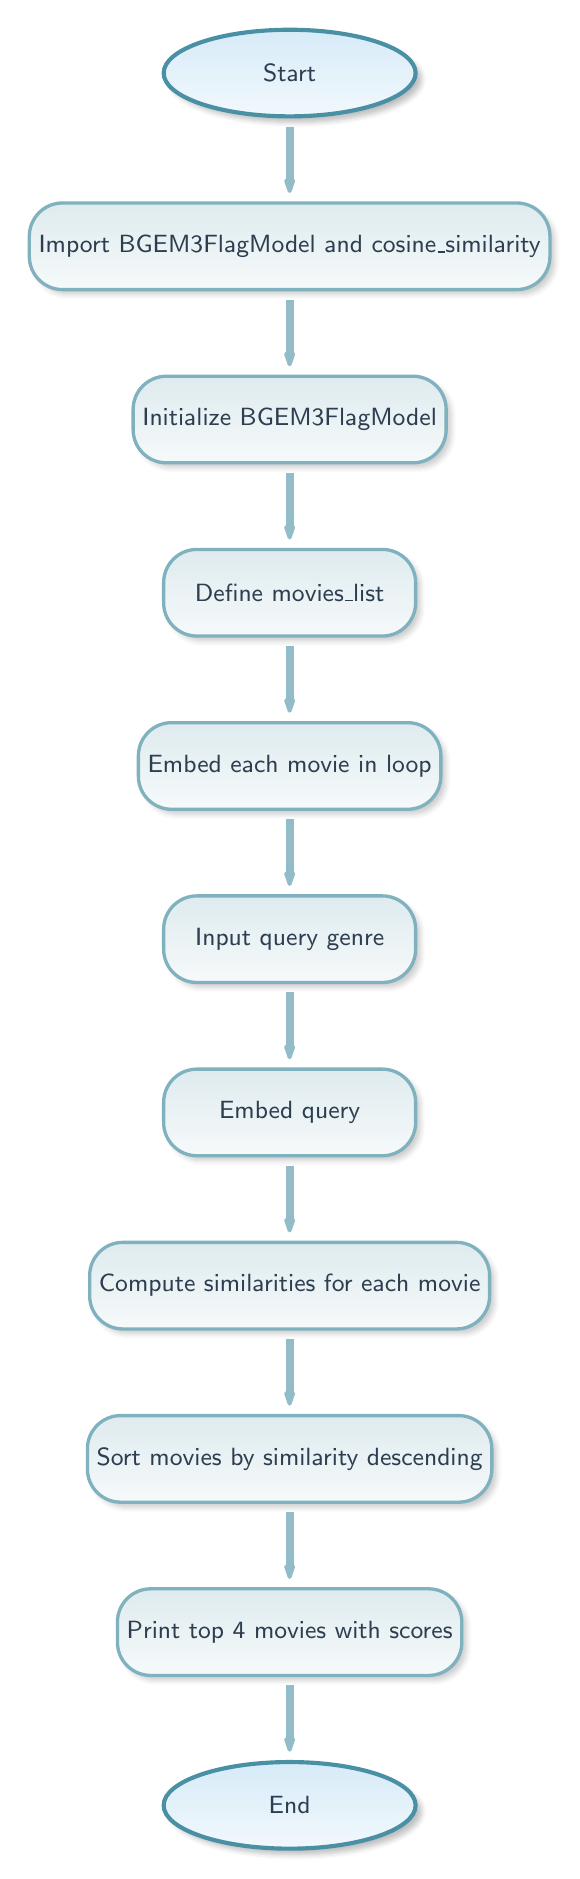
\begin{tikzpicture}[node distance=2.2cm, font=\sffamily\small]
    \node (start) [startstop] {Start};
    \node (import) [process, below of=start] {Import BGEM3FlagModel and cosine\_similarity};
    \node (init) [process, below of=import] {Initialize BGEM3FlagModel};
    \node (movies) [process, below of=init] {Define movies\_list};
    \node (embed_movies) [process, below of=movies] {Embed each movie in loop};
    \node (input) [process, below of=embed_movies] {Input query genre};
    \node (embed_query) [process, below of=input] {Embed query};
    \node (compute) [process, below of=embed_query] {Compute similarities for each movie};
    \node (sort) [process, below of=compute] {Sort movies by similarity descending};
    \node (print) [process, below of=sort] {Print top 4 movies with scores};
    \node (end) [startstop, below of=print] {End};

    \draw [arrow] (start) -- (import);
    \draw [arrow] (import) -- (init);
    \draw [arrow] (init) -- (movies);
    \draw [arrow] (movies) -- (embed_movies);
    \draw [arrow] (embed_movies) -- (input);
    \draw [arrow] (input) -- (embed_query);
    \draw [arrow] (embed_query) -- (compute);
    \draw [arrow] (compute) -- (sort);
    \draw [arrow] (sort) -- (print);
    \draw [arrow] (print) -- (end);
\end{tikzpicture}

\section{Ollama Equivalent Code}

\begin{lstlisting}[language=Python]
from langchain_community.embeddings import HuggingFaceEmbeddings
from sklearn.metrics.pairwise import cosine_similarity

model = HuggingFaceEmbeddings(model_name='BAAI/bge-m3')

movies_list = [
    "Shadow Hunters: ACTION FANTASY THRILLER",
    "Eternal Bonds: DRAMA ROMANCE FAMILY",
    "Neon Horizon: SCI-FI ACTION ADVENTURE",
    "Whispers in the Dark: HORROR MYSTERY THRILLER",
    "Crimson Crown: HISTORICAL WAR DRAMA",
    "Starlight Dreams: ROMANCE COMEDY MUSIC",
    "Code Breakers: TECH THRILLER CRIME",
    "The Lost Kingdom: ADVENTURE ACTION FANTASY",
    "Broken Silence: CRIME DRAMA SUSPENSE",
    "Frozen Ashes: SURVIVAL DRAMA ACTION"
]

# Convert movie list into embeddings
embeddings_list = model.embed_documents(movies_list)

query = input("ENTER THE GENRE FOR WHICH YOU WANT TO SEE MOVIES: ")

query_embedding = model.embed_query(query)

similarity_scores = {}

for i, movie_emb in enumerate(embeddings_list):
    similarity = cosine_similarity(
        [query_embedding],
        [movie_emb]
    )[0][0]

    similarity_scores[movies_list[i]] = similarity

sorted_movies = sorted(similarity_scores.items(), key=lambda x: x[1], reverse=True)

#Retrieved data
print("\n Top Recommended Movies:")
for movie, score in sorted_movies[:4]:
    print(f"{movie}   ---> Similarity: {score:.4f}")
\end{lstlisting}

\subsection{Diff Explanation}

The Ollama equivalent uses LangChain's HuggingFaceEmbeddings wrapper, which simplifies embedding multiple documents and queries with dedicated methods.

Key changes:
\begin{itemize}
    \item \textcolor{red}{Removed:} \texttt{from FlagEmbedding import BGEM3FlagModel}
    \item \textcolor{green}{Added:} \texttt{from langchain\_community.embeddings import HuggingFaceEmbeddings}
    \item \textcolor{red}{Removed:} \texttt{model = BGEM3FlagModel(...)}
    \item \textcolor{green}{Added:} \texttt{model = HuggingFaceEmbeddings(model\_name='BAAI/bge-m3')}
    \item \textcolor{red}{Removed:} Loop to encode each movie
    \item \textcolor{green}{Added:} \texttt{embeddings\_list = model.embed\_documents(movies\_list)}
    \item \textcolor{red}{Removed:} \texttt{model.encode(query)['dense\_vecs']}
    \item \textcolor{green}{Added:} \texttt{query\_embedding = model.embed\_query(query)}
\end{itemize}

These changes leverage LangChain's abstraction for batch document embedding and query embedding, making the code more concise and integrated with LangChain ecosystems, while achieving the same recommendation logic.

\section{Hugging Face Equivalent Code}

\begin{lstlisting}[language=Python]
from FlagEmbedding import BGEM3FlagModel
from sklearn.metrics.pairwise import cosine_similarity

model = BGEM3FlagModel('BAAI/bge-m3', use_fp16=True)

movies_list = [
    "Shadow Hunters: ACTION FANTASY THRILLER",
    "Eternal Bonds: DRAMA ROMANCE FAMILY",
    "Neon Horizon: SCI-FI ACTION ADVENTURE",
    "Whispers in the Dark: HORROR MYSTERY THRILLER",
    "Crimson Crown: HISTORICAL WAR DRAMA",
    "Starlight Dreams: ROMANCE COMEDY MUSIC",
    "Code Breakers: TECH THRILLER CRIME",
    "The Lost Kingdom: ADVENTURE ACTION FANTASY",
    "Broken Silence: CRIME DRAMA SUSPENSE",
    "Frozen Ashes: SURVIVAL DRAMA ACTION"
]

# Convert movie list into embeddings
embeddings_list = []
for movie in movies_list:
    emb = model.encode(
        movie,
        batch_size=12,
        max_length=8192
    )['dense_vecs']
    embeddings_list.append(emb)

query = input("ENTER THE GENRE FOR WHICH YOU WANT TO SEE MOVIES: ")

query_embedding = model.encode(
    query,
    batch_size=12,
    max_length=8192
)['dense_vecs']

similarity_scores = {}

for i, movie_emb in enumerate(embeddings_list):
    similarity = cosine_similarity(
        [query_embedding],
        [movie_emb]
    )[0][0]

    similarity_scores[movies_list[i]] = similarity

sorted_movies = sorted(similarity_scores.items(), key=lambda x: x[1], reverse=True)

#Retrieved data
print("\n Top Recommended Movies:")
for movie, score in sorted_movies[:4]:
    print(f"{movie}   ---> Similarity: {score:.4f}")
\end{lstlisting}

\subsection{Diff Explanation}

The Hugging Face equivalent is nearly identical to the original, using the same BGEM3FlagModel and encoding approach.

Key changes: None significant; the code is essentially the same, with minor formatting differences (e.g., comment "Retrieved data" instead of "Retrived data").

This indicates that for direct Hugging Face usage, the original code is already optimal, requiring no adaptations.


% ===== CODE17 =====
\newpage
\section{Original Code (src/code17.py)}

The original code implements a complete Retrieval-Augmented Generation (RAG) pipeline for movie recommendations, using embeddings for retrieval and an LLM for generation.

\begin{lstlisting}[language=Python]
# ============================================================
# RAG PIPELINE WITH EXTERNAL MOVIE DATASET -- MODULAR VERSION
# ============================================================

# !pip install -U FlagEmbedding langchain-openai python-dotenv

from FlagEmbedding import BGEM3FlagModel
from sklearn.metrics.pairwise import cosine_similarity
from langchain.chat_models import AzureChatOpenAI
from dotenv import load_dotenv
import os

load_dotenv()

# ------------------------------------------------------------
# FUNCTION 1: Load Movie Dataset
# ------------------------------------------------------------
def load_movie_dataset():
    return [
        "Shadow Hunters: ACTION FANTASY THRILLER",
        "Eternal Bonds: DRAMA ROMANCE FAMILY",
        "Neon Horizon: SCI-FI ACTION ADVENTURE",
        "Whispers in the Dark: HORROR MYSTERY THRILLER",
        "Crimson Crown: HISTORICAL WAR DRAMA",
        "Starlight Dreams: ROMANCE COMEDY MUSIC",
        "Code Breakers: TECH THRILLER CRIME",
        "The Lost Kingdom: ADVENTURE ACTION FANTASY",
        "Broken Silence: CRIME DRAMA SUSPENSE",
        "Frozen Ashes: SURVIVAL DRAMA ACTION"
    ]

# ------------------------------------------------------------
# FUNCTION 2: Load Embedding Model + Generate Embeddings
# ------------------------------------------------------------
def embed_movies(movies_list):
    model = BGEM3FlagModel("BAAI/bge-m3", use_fp16=True)
    embeddings = [
        model.encode(movie, batch_size=12, max_length=8192)["dense_vecs"]
        for movie in movies_list
    ]
    return model, embeddings

# ------------------------------------------------------------
# FUNCTION 3: Retrieve Top-K Relevant Movies
# ------------------------------------------------------------
def retrieve_top_movies(query, model, movies_list, movie_embeddings, top_k=4):
    query_emb = model.encode(query, batch_size=12, max_length=8192)["dense_vecs"]

    similarity_scores = {}
    for i, emb in enumerate(movie_embeddings):
        sim = cosine_similarity([query_emb], [emb])[0][0]
        similarity_scores[movies_list[i]] = sim

    sorted_results = sorted(
        similarity_scores.items(), key=lambda x: x[1], reverse=True
    )
    return sorted_results[:top_k]

# ------------------------------------------------------------
# FUNCTION 4: Build the RAG Prompt
# ------------------------------------------------------------
def build_rag_prompt(query, retrieved_movies):
    context_text = "\n".join([f"- {m[0]}" for m in retrieved_movies])

    prompt = f"""
You are a movie recommendation expert.

USER QUERY:
{query}

RETRIEVED MOVIES (Context Provided):
{context_text}

TASK:
Using ONLY the above movies as your context, recommend movies to the user.
Clearly explain why each recommended movie matches the user's taste.
Do NOT mention similarity scores or embeddings.
"""
    return prompt

# ------------------------------------------------------------
# FUNCTION 5: Invoke Azure OpenAI LLM
# ------------------------------------------------------------
def generate_llm_response(prompt):
    llm = AzureChatOpenAI(
        openai_api_base=os.getenv("AZURE_OPENAI_API_BASE"),
        openai_api_version=os.getenv("AZURE_OPENAI_API_VERSION"),
        openai_api_key=os.getenv("AZURE_OPENAI_API_KEY"),
        deployment_name=os.getenv("AZURE_OPENAI_DEPLOYMENT_NAME"),
        model_name="gpt-4o",
        temperature=0.7,
    )

    response = llm.invoke(prompt)
    return response.content

# ------------------------------------------------------------
# FUNCTION 6: Full RAG Pipeline Executor
# ------------------------------------------------------------
def run_rag_pipeline():
    # Load dataset
    movies_list = load_movie_dataset()

    # Embeddings
    model, movie_embeddings = embed_movies(movies_list)

    # User Input
    query = input("Enter movie genre or mood: ")

    # Retrieve
    retrieved = retrieve_top_movies(query, model, movies_list, movie_embeddings)

    # Build prompt
    prompt = build_rag_prompt(query, retrieved)

    # LLM response
    answer = generate_llm_response(prompt)

    print("\n====================== RAG ANSWER ======================")
    print(answer)

# ------------------------------------------------------------
# RUN PIPELINE
# ------------------------------------------------------------
run_rag_pipeline()
\end{lstlisting}

\section{Explanation}

\subsection{What}
This code builds a modular Retrieval-Augmented Generation (RAG) pipeline for movie recommendations. It retrieves relevant movies from a dataset based on semantic similarity to a user query, then uses an LLM to generate personalized recommendations with explanations.

\subsection{Why}
RAG combines the strengths of retrieval (finding relevant information) and generation (creating coherent responses). This prevents hallucinations in LLMs by grounding responses in retrieved data, making recommendations more accurate and contextually relevant.

\subsection{How}
1. Load a dataset of movie descriptions.
2. Embed all movies using BGEM3FlagModel.
3. Take user input for genre/mood.
4. Embed the query and retrieve top-K similar movies via cosine similarity.
5. Build a prompt with the query and retrieved movies as context.
6. Invoke Azure OpenAI GPT-4o to generate a recommendation response.
7. Print the final answer.

The modular structure separates concerns: data loading, embedding, retrieval, prompt building, LLM invocation, and pipeline execution.

\section{Flowchart}

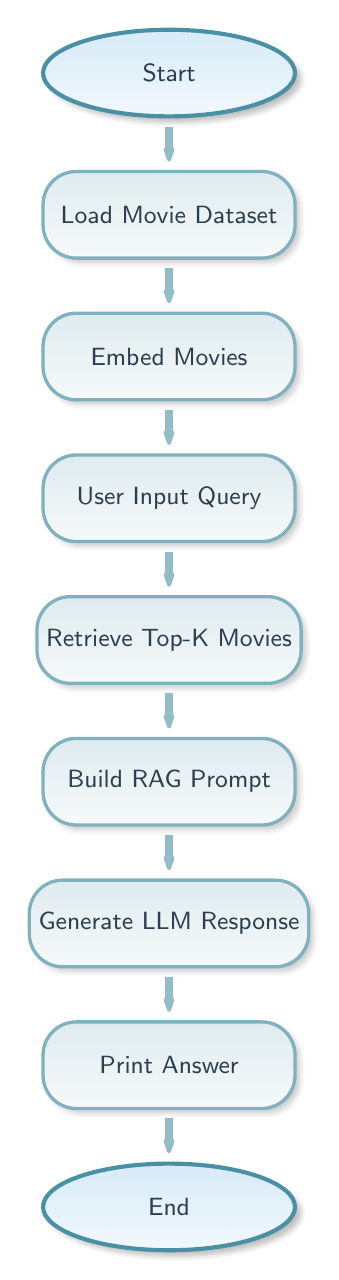
\begin{tikzpicture}[node distance=1.8cm, font=\sffamily\small]
    \node (start) [startstop] {Start};
    \node (load) [process, below of=start] {Load Movie Dataset};
    \node (embed) [process, below of=load] {Embed Movies};
    \node (input) [process, below of=embed] {User Input Query};
    \node (retrieve) [process, below of=input] {Retrieve Top-K Movies};
    \node (build) [process, below of=retrieve] {Build RAG Prompt};
    \node (generate) [process, below of=build] {Generate LLM Response};
    \node (print) [process, below of=generate] {Print Answer};
    \node (end) [startstop, below of=print] {End};

    \draw [arrow] (start) -- (load);
    \draw [arrow] (load) -- (embed);
    \draw [arrow] (embed) -- (input);
    \draw [arrow] (input) -- (retrieve);
    \draw [arrow] (retrieve) -- (build);
    \draw [arrow] (build) -- (generate);
    \draw [arrow] (generate) -- (print);
    \draw [arrow] (print) -- (end);
\end{tikzpicture}

\section{Ollama Equivalent Code}

\begin{lstlisting}[language=Python]
# ============================================================
# RAG PIPELINE WITH EXTERNAL MOVIE DATASET -- MODULAR VERSION
# ============================================================

from langchain_community.embeddings import HuggingFaceEmbeddings
from sklearn.metrics.pairwise import cosine_similarity
from langchain_ollama import OllamaLLM

# ------------------------------------------------------------
# FUNCTION 1: Load Movie Dataset
# ------------------------------------------------------------
def load_movie_dataset():
    return [
        "Shadow Hunters: ACTION FANTASY THRILLER",
        "Eternal Bonds: DRAMA ROMANCE FAMILY",
        "Neon Horizon: SCI-FI ACTION ADVENTURE",
        "Whispers in the Dark: HORROR MYSTERY THRILLER",
        "Crimson Crown: HISTORICAL WAR DRAMA",
        "Starlight Dreams: ROMANCE COMEDY MUSIC",
        "Code Breakers: TECH THRILLER CRIME",
        "The Lost Kingdom: ADVENTURE ACTION FANTASY",
        "Broken Silence: CRIME DRAMA SUSPENSE",
        "Frozen Ashes: SURVIVAL DRAMA ACTION"
    ]

# ------------------------------------------------------------
# FUNCTION 2: Load Embedding Model + Generate Embeddings
# ------------------------------------------------------------
def embed_movies(movies_list):
    model = HuggingFaceEmbeddings(model_name="BAAI/bge-m3")
    embeddings = model.embed_documents(movies_list)
    return model, embeddings

# ------------------------------------------------------------
# FUNCTION 3: Retrieve Top-K Relevant Movies
# ------------------------------------------------------------
def retrieve_top_movies(query, model, movies_list, movie_embeddings, top_k=4):
    query_emb = model.embed_query(query)

    similarity_scores = {}
    for i, emb in enumerate(movie_embeddings):
        sim = cosine_similarity([query_emb], [emb])[0][0]
        similarity_scores[movies_list[i]] = sim

    sorted_results = sorted(
        similarity_scores.items(), key=lambda x: x[1], reverse=True
    )
    return sorted_results[:top_k]

# ------------------------------------------------------------
# FUNCTION 4: Build the RAG Prompt
# ------------------------------------------------------------
def build_rag_prompt(query, retrieved_movies):
    context_text = "\n".join([f"- {m[0]}" for m in retrieved_movies])

    prompt = f"""
You are a movie recommendation expert.

USER QUERY:
{query}

RETRIEVED MOVIES (Context Provided):
{context_text}

TASK:
Using ONLY the above movies as your context, recommend movies to the user.
Clearly explain why each recommended movie matches the user's taste.
Do NOT mention similarity scores or embeddings.
"""
    return prompt

# ------------------------------------------------------------
# FUNCTION 5: Invoke Ollama LLM
# ------------------------------------------------------------
def generate_llm_response(prompt):
    llm = OllamaLLM(model="qwen3:4b", temperature=0.7)

    response = llm.invoke(prompt)
    return response

# ------------------------------------------------------------
# FUNCTION 6: Full RAG Pipeline Executor
# ------------------------------------------------------------
def run_rag_pipeline():
    # Load dataset
    movies_list = load_movie_dataset()

    # Embeddings
    model, movie_embeddings = embed_movies(movies_list)

    # User Input
    query = input("Enter movie genre or mood: ")

    # Retrieve
    retrieved = retrieve_top_movies(query, model, movies_list, movie_embeddings)

    # Build prompt
    prompt = build_rag_prompt(query, retrieved)

    # LLM response
    answer = generate_llm_response(prompt)

    print("\n====================== RAG ANSWER ======================")
    print(answer)

# ------------------------------------------------------------
# RUN PIPELINE
# ------------------------------------------------------------
run_rag_pipeline()
\end{lstlisting}

\subsection{Diff Explanation}

The Ollama equivalent adapts the pipeline to use local models: HuggingFaceEmbeddings for retrieval and OllamaLLM for generation.

Key changes:
\begin{itemize}
    \item \textcolor{red}{Removed:} \texttt{from FlagEmbedding import BGEM3FlagModel}
    \item \textcolor{red}{Removed:} \texttt{from langchain.chat\_models import AzureChatOpenAI}
    \item \textcolor{green}{Added:} \texttt{from langchain\_community.embeddings import HuggingFaceEmbeddings}
    \item \textcolor{green}{Added:} \texttt{from langchain\_ollama import OllamaLLM}
    \item \textcolor{red}{Removed:} BGEM3FlagModel initialization
    \item \textcolor{green}{Added:} \texttt{model = HuggingFaceEmbeddings(model\_name="BAAI/bge-m3")}
    \item \textcolor{red}{Removed:} \texttt{model.encode} for embeddings
    \item \textcolor{green}{Added:} \texttt{model.embed\_documents} and \texttt{embed\_query}
    \item \textcolor{red}{Removed:} AzureChatOpenAI with env vars
    \item \textcolor{green}{Added:} \texttt{llm = OllamaLLM(model="qwen3:4b", temperature=0.7)}
    \item \textcolor{red}{Removed:} \texttt{response.content}
    \item \textcolor{green}{Added:} \texttt{return response} (direct string)
\end{itemize}

These changes enable fully local execution, avoiding cloud dependencies for privacy and cost, while maintaining the same modular RAG structure.

\section{Hugging Face Equivalent Code}

\begin{lstlisting}[language=Python]
# ============================================================
# RAG PIPELINE WITH EXTERNAL MOVIE DATASET -- MODULAR VERSION
# ============================================================

from FlagEmbedding import BGEM3FlagModel
from sklearn.metrics.pairwise import cosine_similarity
from transformers import pipeline

# ------------------------------------------------------------
# FUNCTION 1: Load Movie Dataset
# ------------------------------------------------------------
def load_movie_dataset():
    return [
        "Shadow Hunters: ACTION FANTASY THRILLER",
        "Eternal Bonds: DRAMA ROMANCE FAMILY",
        "Neon Horizon: SCI-FI ACTION ADVENTURE",
        "Whispers in the Dark: HORROR MYSTERY THRILLER",
        "Crimson Crown: HISTORICAL WAR DRAMA",
        "Starlight Dreams: ROMANCE COMEDY MUSIC",
        "Code Breakers: TECH THRILLER CRIME",
        "The Lost Kingdom: ADVENTURE ACTION FANTASY",
        "Broken Silence: CRIME DRAMA SUSPENSE",
        "Frozen Ashes: SURVIVAL DRAMA ACTION"
    ]

# ------------------------------------------------------------
# FUNCTION 2: Load Embedding Model + Generate Embeddings
# ------------------------------------------------------------
def embed_movies(movies_list):
    model = BGEM3FlagModel("BAAI/bge-m3", use_fp16=True)
    embeddings = [
        model.encode(movie, batch_size=12, max_length=8192)["dense_vecs"]
        for movie in movies_list
    ]
    return model, embeddings

# ------------------------------------------------------------
# FUNCTION 3: Retrieve Top-K Relevant Movies
# ------------------------------------------------------------
def retrieve_top_movies(query, model, movies_list, movie_embeddings, top_k=4):
    query_emb = model.encode(query, batch_size=12, max_length=8192)["dense_vecs"]

    similarity_scores = {}
    for i, emb in enumerate(movie_embeddings):
        sim = cosine_similarity([query_emb], [emb])[0][0]
        similarity_scores[movies_list[i]] = sim

    sorted_results = sorted(
        similarity_scores.items(), key=lambda x: x[1], reverse=True
    )
    return sorted_results[:top_k]

# ------------------------------------------------------------
# FUNCTION 4: Build the RAG Prompt
# ------------------------------------------------------------
def build_rag_prompt(query, retrieved_movies):
    context_text = "\n".join([f"- {m[0]}" for m in retrieved_movies])

    prompt = f"""
You are a movie recommendation expert.

USER QUERY:
{query}

RETRIEVED MOVIES (Context Provided):
{context_text}

TASK:
Using ONLY the above movies as your context, recommend movies to the user.
Clearly explain why each recommended movie matches the user's taste.
Do NOT mention similarity scores or embeddings.
"""
    return prompt

# ------------------------------------------------------------
# FUNCTION 5: Invoke HF LLM
# ------------------------------------------------------------
def generate_llm_response(prompt):
    pipe = pipeline("text-generation", model="Qwen/Qwen3-0.6B")

    result = pipe(prompt, max_new_tokens=200, temperature=0.7, num_return_sequences=1)
    return result[0]['generated_text']

# ------------------------------------------------------------
# FUNCTION 6: Full RAG Pipeline Executor
# ------------------------------------------------------------
def run_rag_pipeline():
    # Load dataset
    movies_list = load_movie_dataset()

    # Embeddings
    model, movie_embeddings = embed_movies(movies_list)

    # User Input
    query = input("Enter movie genre or mood: ")

    # Retrieve
    retrieved = retrieve_top_movies(query, model, movies_list, movie_embeddings)

    # Build prompt
    prompt = build_rag_prompt(query, retrieved)

    # LLM response
    answer = generate_llm_response(prompt)

    print("\n====================== RAG ANSWER ======================")
    print(answer)

# ------------------------------------------------------------
# RUN PIPELINE
# ------------------------------------------------------------
run_rag_pipeline()
\end{lstlisting}

\subsection{Diff Explanation}

The Hugging Face equivalent uses direct Hugging Face libraries: BGEM3FlagModel for embeddings and transformers pipeline for text generation.

Key changes:
\begin{itemize}
    \item \textcolor{red}{Removed:} LangChain imports for LLM
    \item \textcolor{green}{Added:} \texttt{from transformers import pipeline}
    \item \textcolor{red}{Removed:} AzureChatOpenAI or OllamaLLM
    \item \textcolor{green}{Added:} \texttt{pipe = pipeline("text-generation", model="Qwen/Qwen3-0.6B")}
    \item \textcolor{red}{Removed:} \texttt{llm.invoke(prompt)}
    \item \textcolor{green}{Added:} \texttt{pipe(prompt, max\_new\_tokens=200, ...)}
    \item \textcolor{red}{Removed:} \texttt{response.content}
    \item \textcolor{green}{Added:} \texttt{result[0]['generated\_text']}
\end{itemize}

These changes use native Hugging Face tools for both embedding and generation, providing more control over model parameters and avoiding LangChain abstractions for direct integration.

\end{document}

